
\chapter{W+bb Cross Section Measurement [TODO - WESLEY COMMENTS / CUTFLOW] }\label{sec:wbbxc}

We now have the tools in place to examine the first of the
 two Standard Model (SM) processes investigated in this text.
This process is \ppwbb at \s 8 \TeV with colliding protons
 provided by the Large Hadron Collider and detected
 by the Compact Muon Solenoid experiment. 

\section{Previous Measurements}

The production of \z bosons
 \cite{Chatrchyan:2012vr,Chatrchyan:2014dha,Chatrchyan:2013zja,Aad:2011jn,Aad:2014dvb}
 or \w bosons \cite{Chatrchyan:2013uza,Aad:2013vka}
 in association with b jets has been 
 studied at a center-of-mass
 energy of 7 TeV using data samples with up
 to 5 \fbinv of integrated luminosity,
 by the ATLAS and CMS experiments, 
 as well as at 
 the Tevatron \cite{WbbTevD0,WbbTevCDF} at $\sqrt{s}=1.96$ TeV. 
This analysis extends previous measurements of the \wbb cross section \cite{Chatrchyan:2013uza},
 using data at $\sqrt{s}=8 \TeV$, collected by the CMS detector in 2012 
 and corresponding to an integrated luminosity of 19.8 \fbinv \cite{ref:CMSLumiCalc}.
 %=====expand=======

\section{Event Selection}

 Two decay channels of the \w boson are considered,
  $\w\rightarrow \mu\nu_\mu$ and $\w\rightarrow e\nu_e$,
 and events are selected using
 single-muon (single-electron) triggers with a
 loosely isolated muon (electron)
 with transverse momentum $\pt>24~(27)$ \GeV
 and pseudo-rapidity $\abs{\eta}<2.1~(2.5)$.
Individual particles emerging from each collision are then reconstructed with the
 particle-flow (PF) technique described in Section \ref{sec:particleflow}
 which ultimately has the effect of dividing them 
 into mutually exclusive categories:
 charged and neutral hadrons, photons, electrons, and muons.

Both the muon and electron candidates are required to have 
 $\pt$ larger than 30 \GeV and $\abs{\eta}<2.1$ and
 to originate from the primary vertex of the event,
 chosen as the vertex with the highest $\sum \pt^2$
 of the charged particles associated with it.
These leptons must additionally pass a tight ID requirement 
 described in Section \ref{sec:leptonid},
 and  must be isolated where
 the isolation variable is defined as

\begin{equation}
\label{eq:iso}
I =\frac{ \sum\pt^{\mathrm{charged}}+{\mathrm{max}}(0,\sum\pt^{\gamma}+\sum\et^{\mathrm{neutral}}-0.5\cdot\pt^{\mathrm{PU}})}{\pt^\ell},
\end{equation}
 with the sum running over the PF candidates (hadrons, electrons, photons)
 in a cone of size $\Delta R < 0.4~(0.3)$ around the muon (electron) direction.
 %where $\Delta R = \sqrt {\smash[b]{ (\Delta \eta)^2 + (\Delta \phi)^2}}$.
The isolation includes a correction for pileup effects,
 which is based on the scalar sum of transverse momenta of charged particles
 not associated with the primary vertex in the isolation cone 
 ($\pt^{\mathrm{PU}}$).
The selected muons (electrons) are required to
 have $I < 0.12~(0.10)$.

Missing transverse energy, $\vmet$, is defined in Section \ref{sec:met}
 as the negative vector sum of the transverse momenta
 of all reconstructed particle candidates in the event.
 It is  combined with the $\pt$ of a muon or electron passing
 the identification and isolation requirements to form a $\w$ candidate.
%Assuming a negligible lepton mass, the transverse mass, $\mt$, of the W is defined as 
%
% \begin{equation}
% \mt^2 = 2 E_T^{\mathrm{miss}} \pt^\ell \left(1-\cos\Delta\phi\right) % massless lepton approximation
% \end{equation}
% where $\Delta\phi$ is the azimuthal angle between the lepton $\vec{\pt}$
% and $\vmet$.
The transverse mass of the \w boson, as defined in Section \ref{sec:transversemass},
  is a  natural discriminator against non-$\w$ final states
 such as QCD multijet events,
 that have a lepton candidate and $\vmet$,
 but a relatively low value of $\mt$.
In calculating \mt, the \met is corrected for noise in the
 electromagnetic and hadron calorimeters \cite{WZCMS:2010}.
 and corrections to mitigate the effect of the
 pileup are also included \cite{CMS:8TeVMET}.

Jets are constructed using the anti-$k_t$ clustering algorithm \cite{Cacciari:2008gp},
 as implemented in the \textsc{fastjet} package \cite{fastjet1,fastjet2},
 with a distance parameter of 0.5.
Jet clustering is performed using individual particle candidates reconstructed with the PF technique.
Jets are required to pass identification
 criteria that eliminate jets originating from
 noisy channels in the hadron calorimeter \cite{Chatrchyan:2009hy}.
Those which originate from pileup interactions are
 rejected by requiring consistency of the jets
 with the primary interaction vertex.
Small corrections to the relative and absolute jet energy calibrations of the detector are
 applied as a function of the $\pt$ and $\eta$  of the jet \cite{cmsJEC}.

The combined secondary vertex (CSV) b-tagging algorithm \cite{CMS-PAS-BTV-13-001,cmsBTAGPAPER} exploits
 the long lifetime and relatively large mass of b hadrons to provide optimized
 b jet discrimination.
The CSV algorithm combines information about impact parameter
 significance, secondary vertex (SV) kinematic properties, and jet kinematic
 properties in a likelihood-ratio technique.
The tagging of a jet is made by imposing a minimum threshold on
 the CSV discriminator value and in this analysis we require
 that both jets pass a threshold which has a b-tagging
 efficiency of about 40\% and a misidentification probability of
 %efficiency of about 50\% and a misidentification probability of
 0.1\% for light jets and 1\% for charm jets.
The scale factors used to correct for the differences in efficiency
 between data and simulation take into account dependencies on
 the transverse momentum of the jet.

After all selection requirements for the signal enhanced dataset are applied,
 the contributing processes to the overall yield are the
 associated production of a massive vector boson and jets ($\vjets$),
 as well as diboson ($\WW$, $\WZ$, $\ZZ$), $\ttbar$, single top, $\gjets$, and QCD multijet production.
The corresponding contributions are estimated from simulation except for QCD, which
 is estimated from data as described in Section \ref{sec:qcd}.
To prove the validity of the MC shapes and normalizations a set of control regions is 
 provided for the background contributions.

\section{Background Estimation}

\subsection{QCD}
\label{sec:qcd}
The QCD multijet sample derived using a data-driven method. 
The shapes of the distributions for QCD multijet events are taken as the difference between
 the data sample and the sum of the other simulated backgrounds in a region of phase
 space enriched in multijets.
The shape of the QCD used in the signal region comes from the distributions 
 illustrated in Fig. \ref{fig:qcdshape}.
This region is found using the same selection requirements as those in the signal region,
 but requiring the muon (electron) to be antiisolated: $I > 0.20 \; (0.15)$.
In the fiducial regions used in this analysis, minimal correlation
 is observed between $I$ and $\mt$, validating
 the use of an inverted isolation requirement to obtain
 the QCD shape.
This shape is then scaled by $ (d_{20}-m_{20})/q_{20} $ where
 $d_{20}$ is the yield in data in the range $0<\mt<20$, $m_{20}$ is the combined
 yield from the simluated samples in this range, and $q_{20}$ is the corresponding
 unnormalized yield of QCD multijet.
This has the effect of normalizing the QCD sample such that the combination of the QCD 
 and the simulated backgrounds has the same total yield as data in the range $0<\mt<20$.
If $d_{20}<m_{20}$, the QCD contribution is taken to be negligable. % and is scaled by $10^{-6}$.
% this happens for ttbar multi-lepton
The relative uncertainty in the yield of QCD multijet events is
 estimated to be $\pm$50\%, taking into account both the fit result
 and the extrapolation from $0<\mt<20$ to the high-$\mt$ range.
This relative uncertainty also covers shape mismodelings
 of the multijet contribution in the final sample.


\begin{figure}
 \caption[QCD shape for \wbb analysis]
 {The shape for the QCD is found by inverting the lepton
  isolation and subtracting MC from the data.
  Shown above is the data, MC background and 
   extrapolated QCD shape (difference between data
   and MC backbrounds) in this inverted
   region for both the muon and electron channels
   in the $W+jj$ and $W+b\bar{b}$ phase spaces.
  The requirement of two well-identified b tags
   essentially eliminates all MC backgrounds in
   the $W+b\bar{b}$ region, leaving the QCD shape 
   the same as that of the data.
  }
 \center
\label{fig:qcd_mu}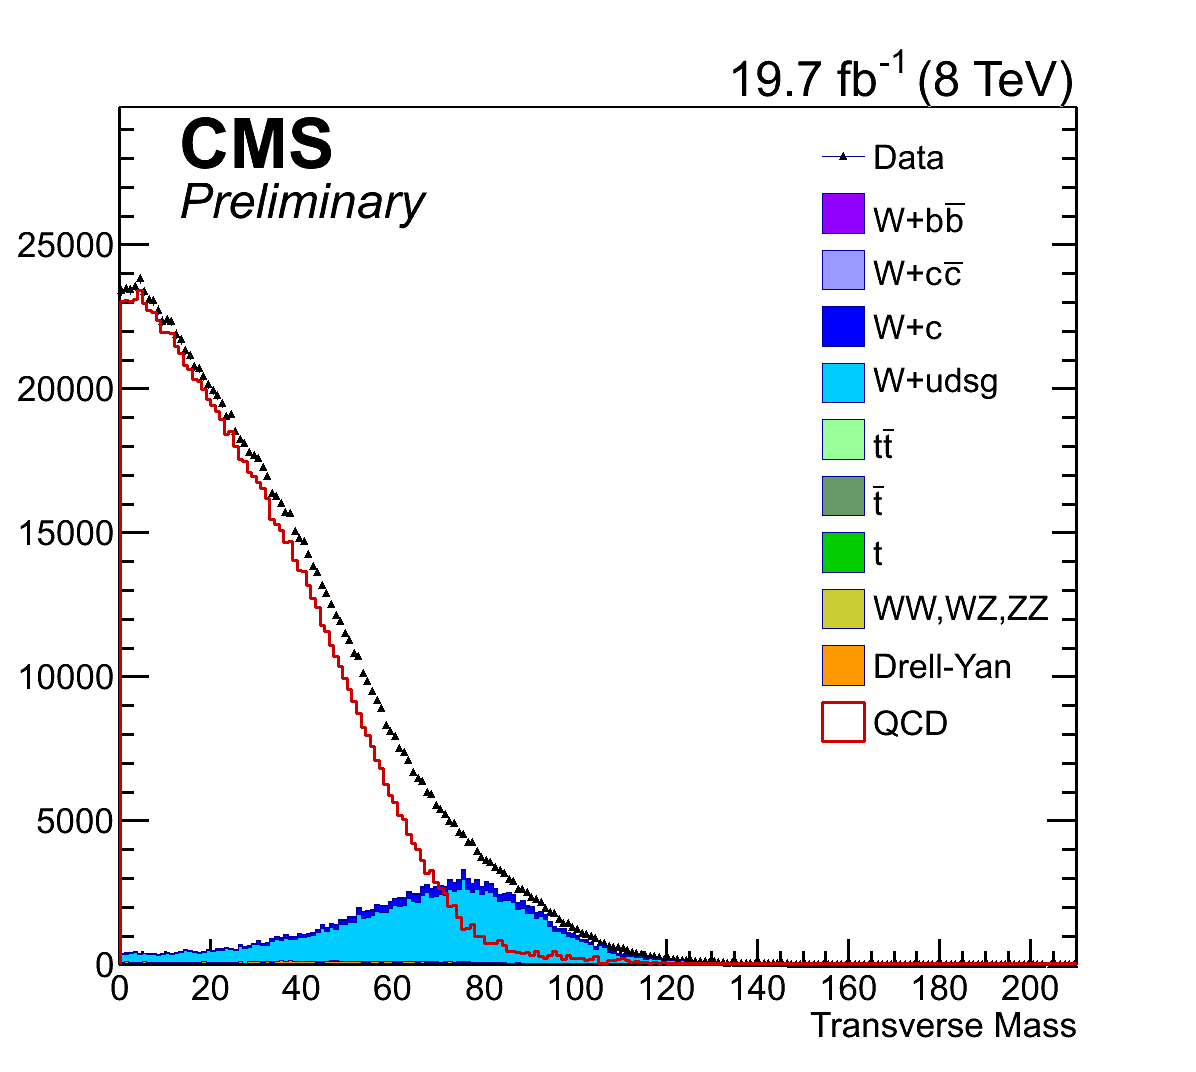
\includegraphics[width=0.4\textwidth]{/Users/rhombus/CMS/Thesis/thesis/pdfs/wbbxc/qcd/QCDShape_wjj_mt_mu.png}
\label{fig:qcd_mu}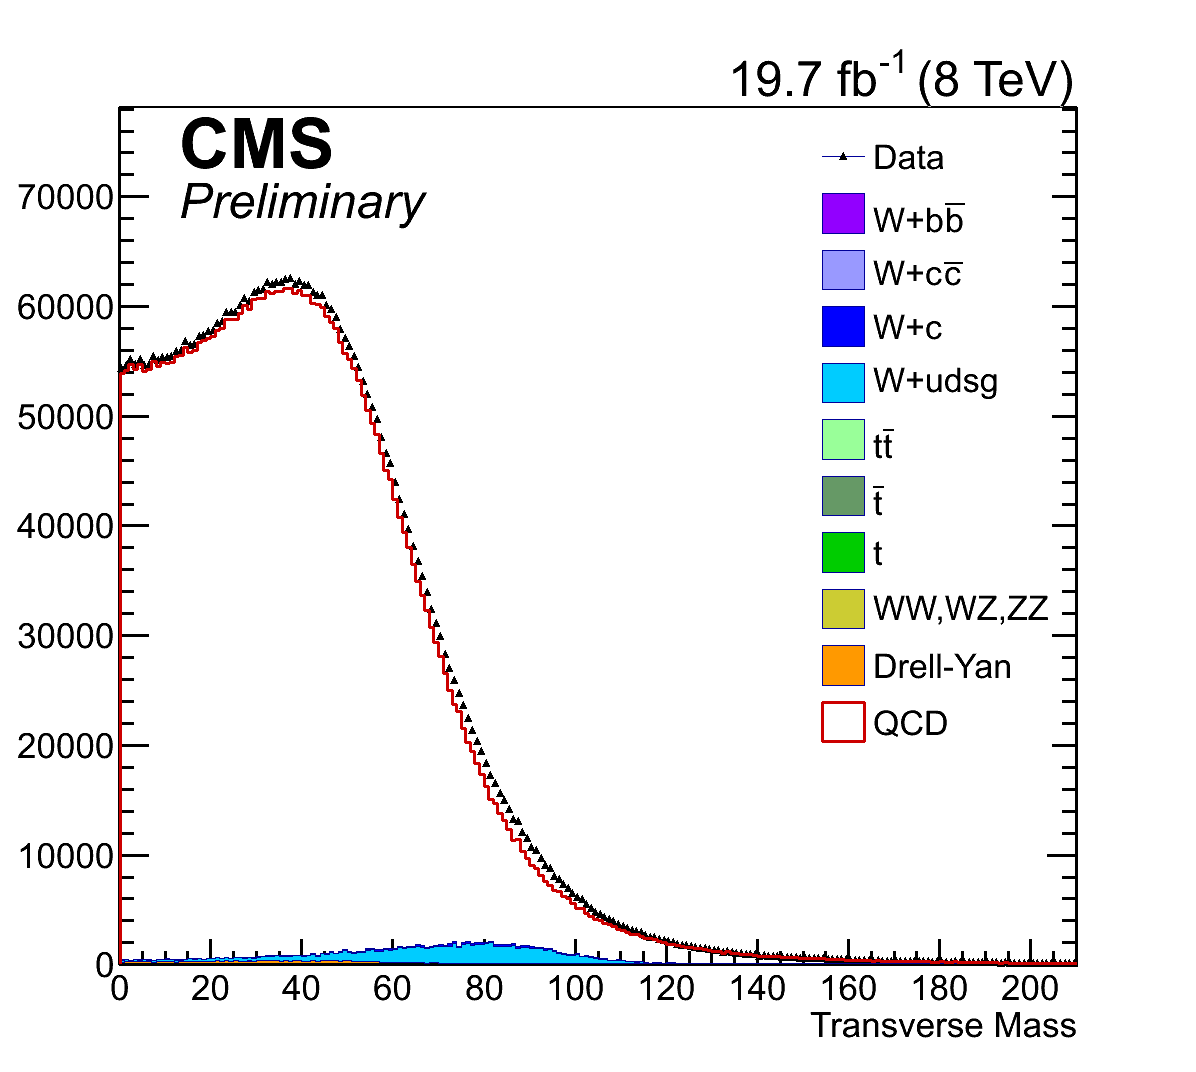
\includegraphics[width=0.4\textwidth]{/Users/rhombus/CMS/Thesis/thesis/pdfs/wbbxc/qcd/QCDShape_wjj_mt_ele.png}
\label{fig:qcd_mu}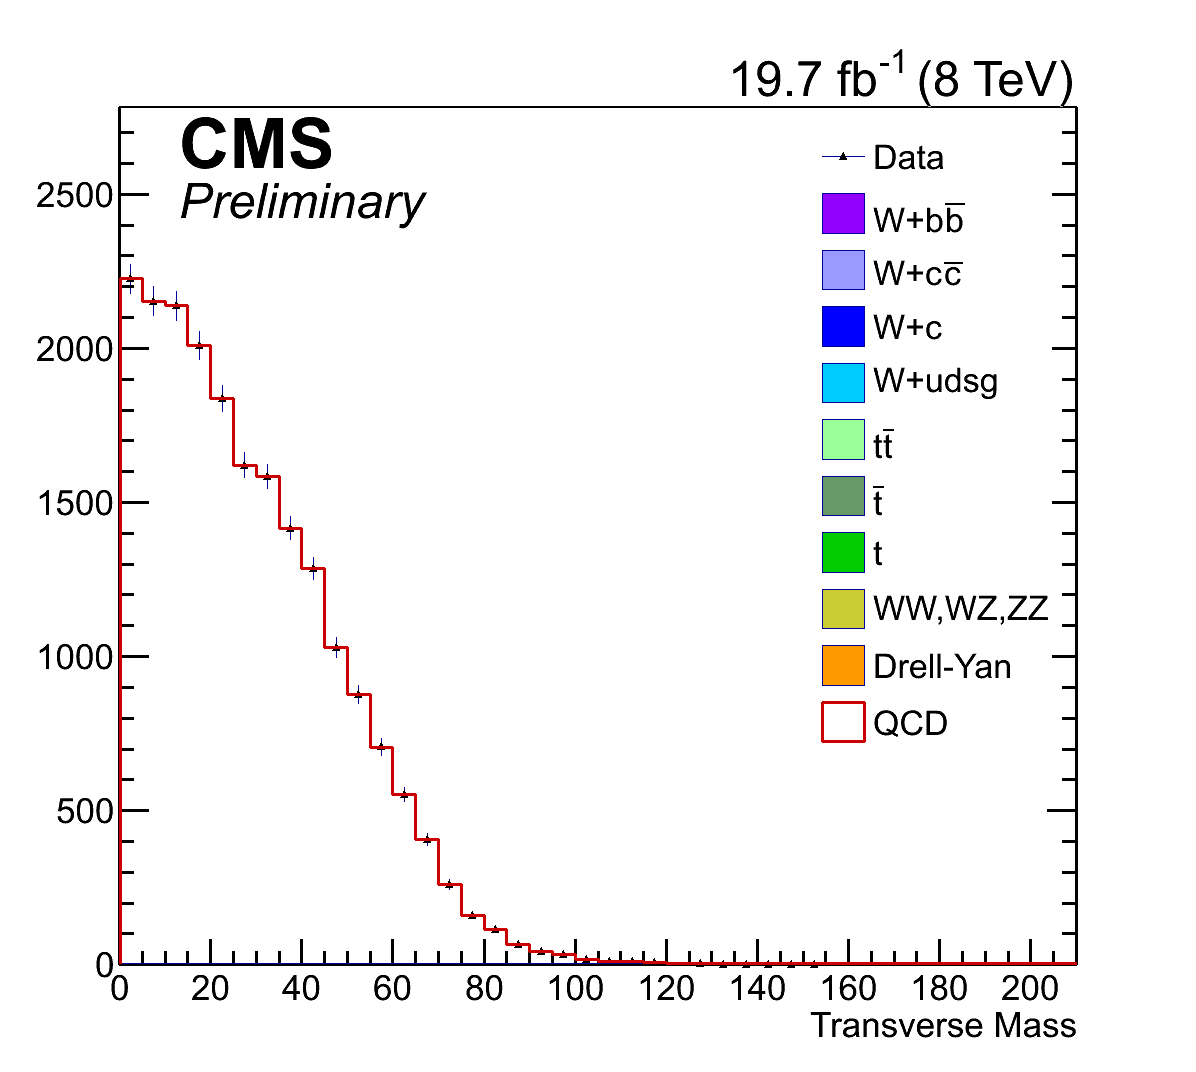
\includegraphics[width=0.4\textwidth]{/Users/rhombus/CMS/Thesis/thesis/pdfs/wbbxc/qcd/QCDShape_wbb_mt_mu_05.png}
\label{fig:qcd_mu}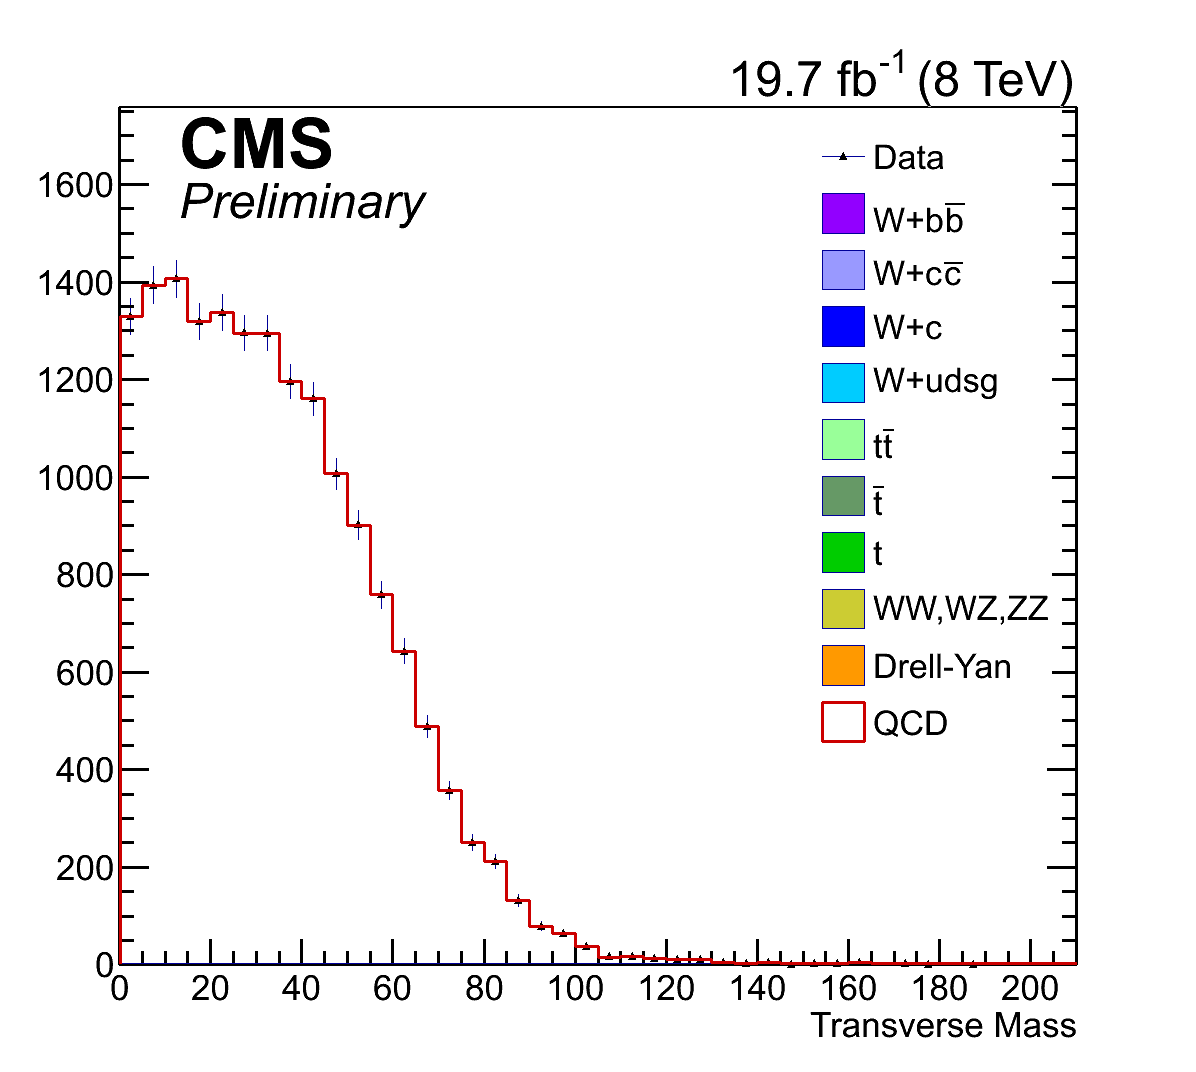
\includegraphics[width=0.4\textwidth]{/Users/rhombus/CMS/Thesis/thesis/pdfs/wbbxc/qcd/QCDShape_wbb_mt_ele_05.png}
 \label{fig:qcdshape}
\end{figure}



\subsection{W+jets: light and charm component}

$W$+jets is the dominating background in the $W+jj$ phase space,
 which is found using idential selections as are used in 
 the signal region with the exception of the b tag requirement;
 in the $W+jj$ phase space, no requirements on b tags are made.
This control region therefore serves as a cross check on the 
 reconstructed objects observed in the signal region before
 the added complication of b tagging has been introduced. 
In Figure~\ref{fig:wjj_plots} is shown the \pt 
 of the identified lepton along with the \met and \mt
 in both decay channels.
Agreement between simulation and data is on the order of 10\%.

\begin{figure}
 \caption[\wjj control region for the \wbb measurement]{
  Selecting for a tight ID muon with $\pt>$30 GeV and exactly two central jets passing loose ID,
   we recover the distributions shown above. 
  Shown in the upper left (right)
   is the momentum of the leading lepton in the muon (electron) channel.
  The missing transverse energy is shown in the center,
  and transverse mass is given in the bottom two distributions.
  The shaded band in ratio plots shows statistical uncertainty. 
 } 
 \center
 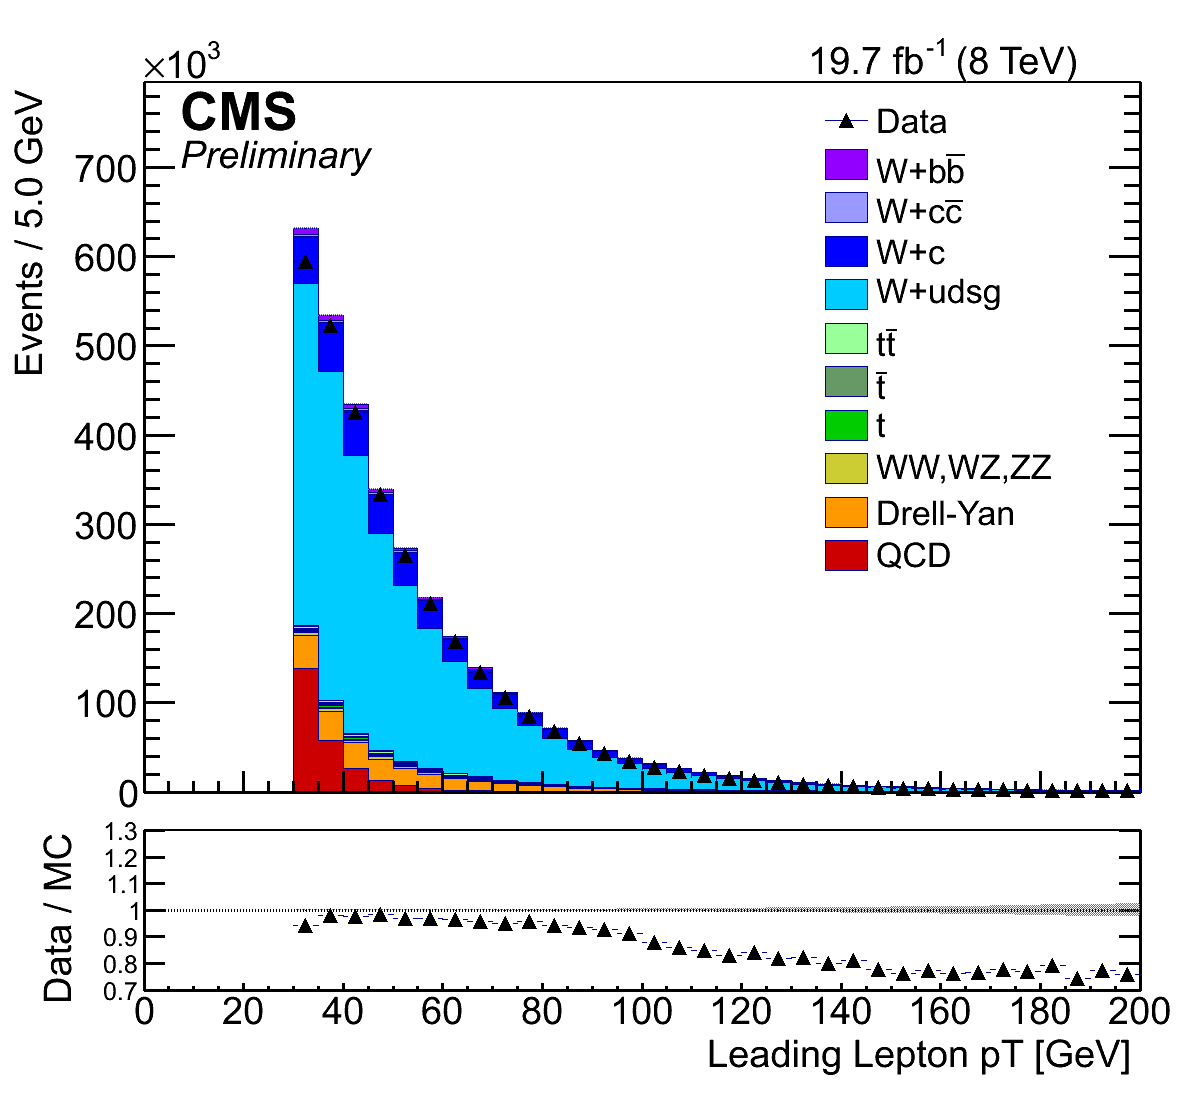
\includegraphics[width=0.4\textwidth]{/Users/rhombus/CMS/Thesis/thesis/pdfs/wbbxc/wjj/Histograms_wjj_goodLep_pt_mu.png}
 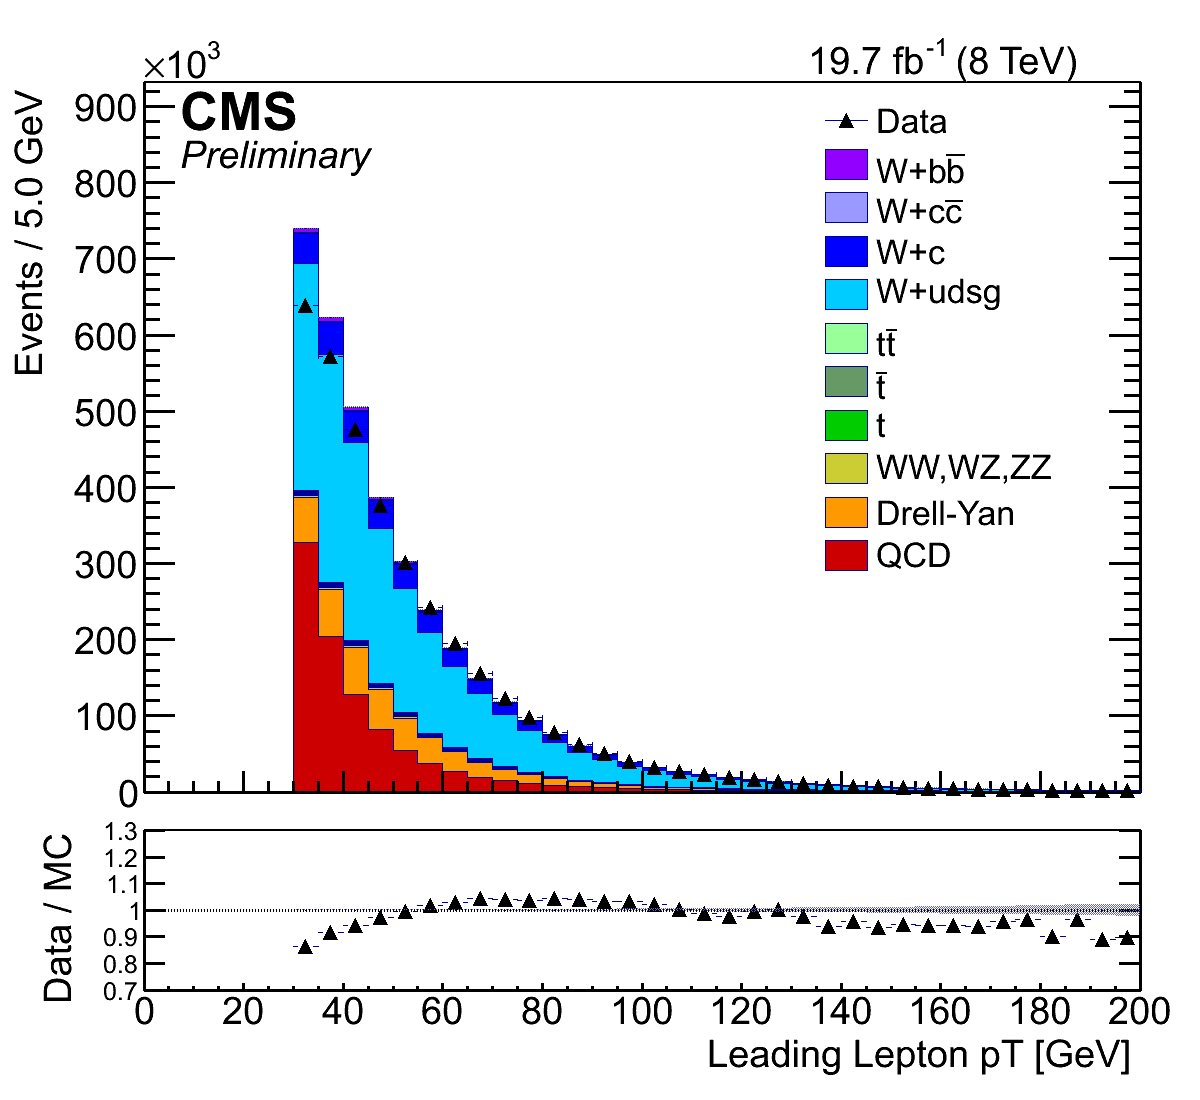
\includegraphics[width=0.4\textwidth]{/Users/rhombus/CMS/Thesis/thesis/pdfs/wbbxc/wjj/Histograms_wjj_goodLep_pt_ele.png}
 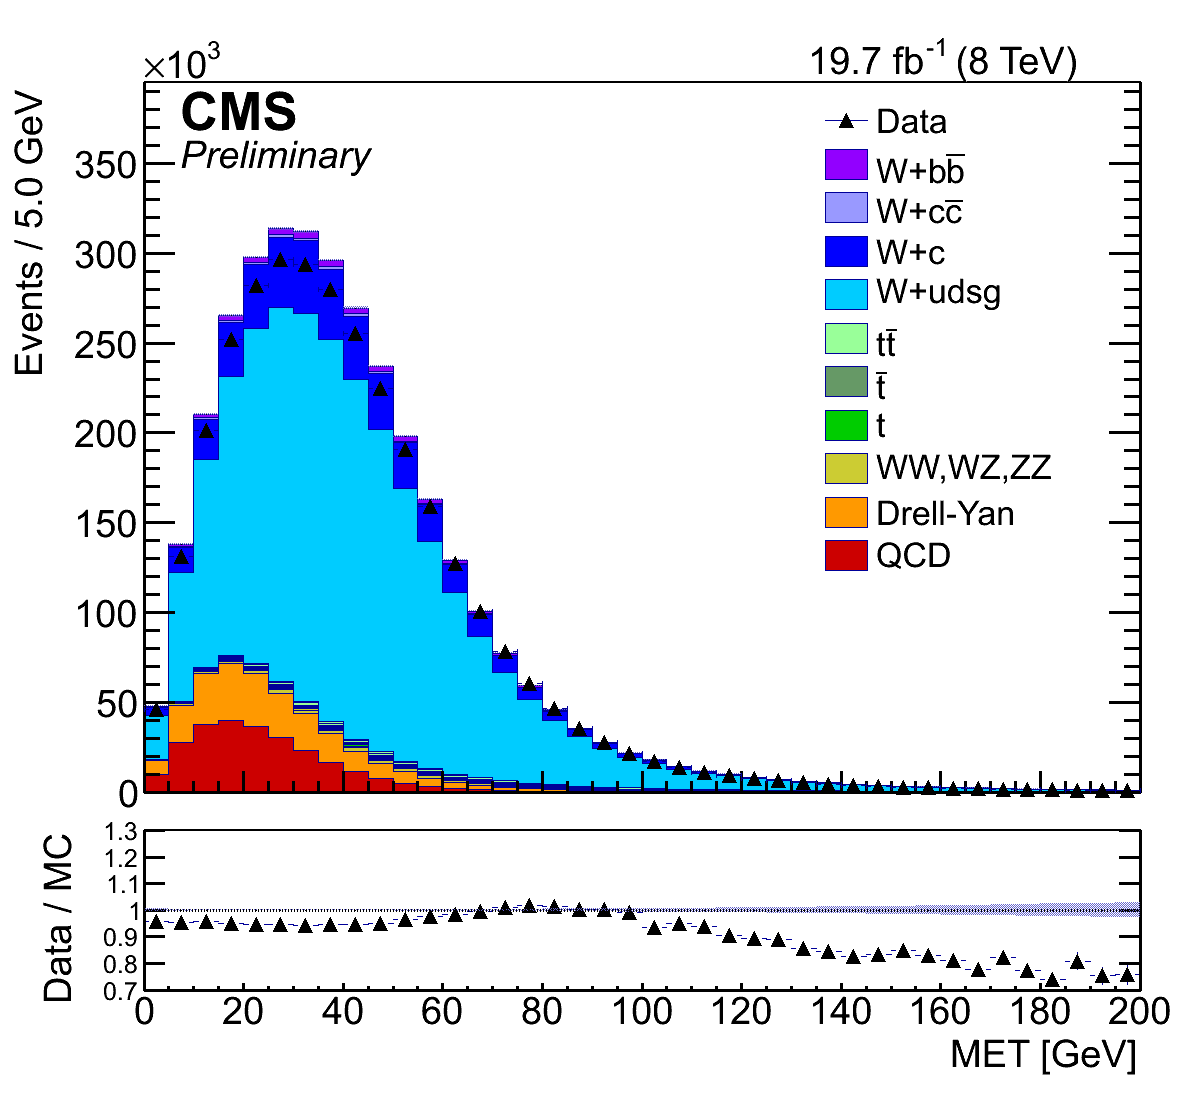
\includegraphics[width=0.4\textwidth]{/Users/rhombus/CMS/Thesis/thesis/pdfs/wbbxc/wjj/Histograms_wjj_met_mu.png}
 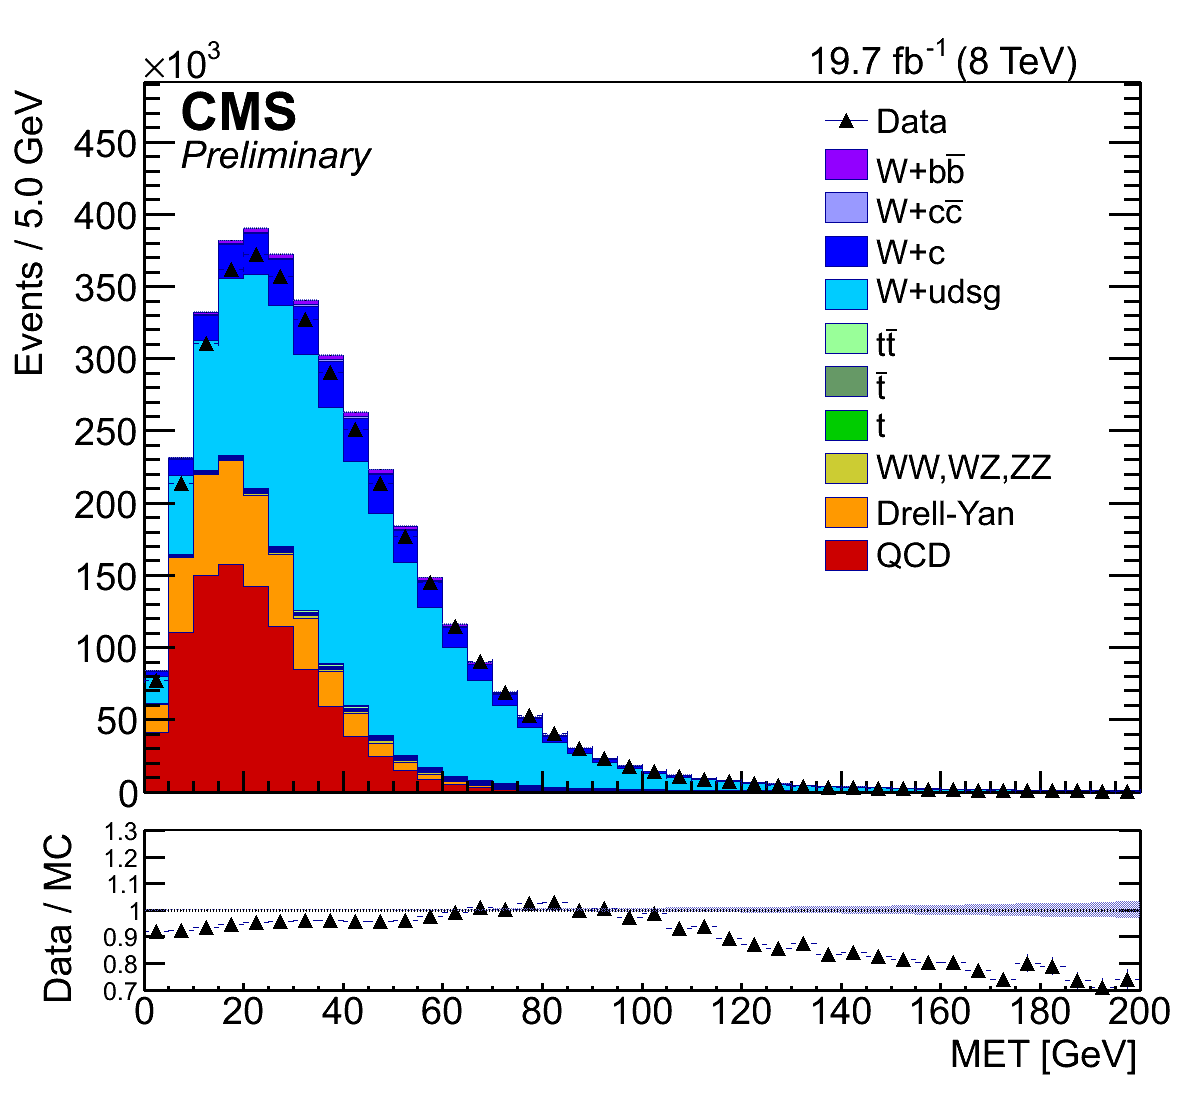
\includegraphics[width=0.4\textwidth]{/Users/rhombus/CMS/Thesis/thesis/pdfs/wbbxc/wjj/Histograms_wjj_met_ele.png}
 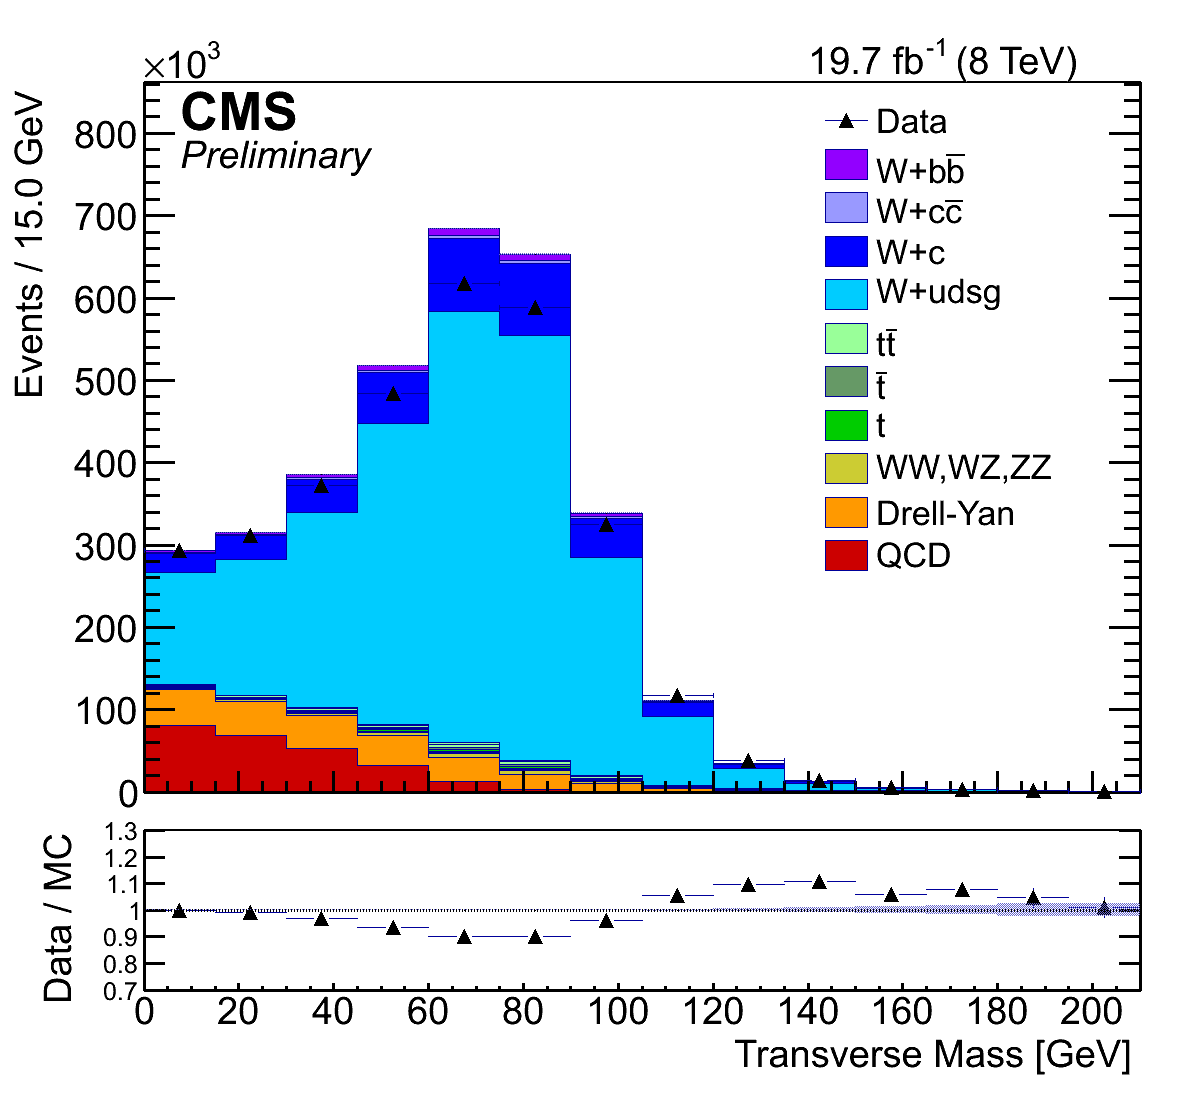
\includegraphics[width=0.4\textwidth]{/Users/rhombus/CMS/Thesis/thesis/pdfs/wbbxc/wjj/Histograms_wjj_mt_mu.png}
 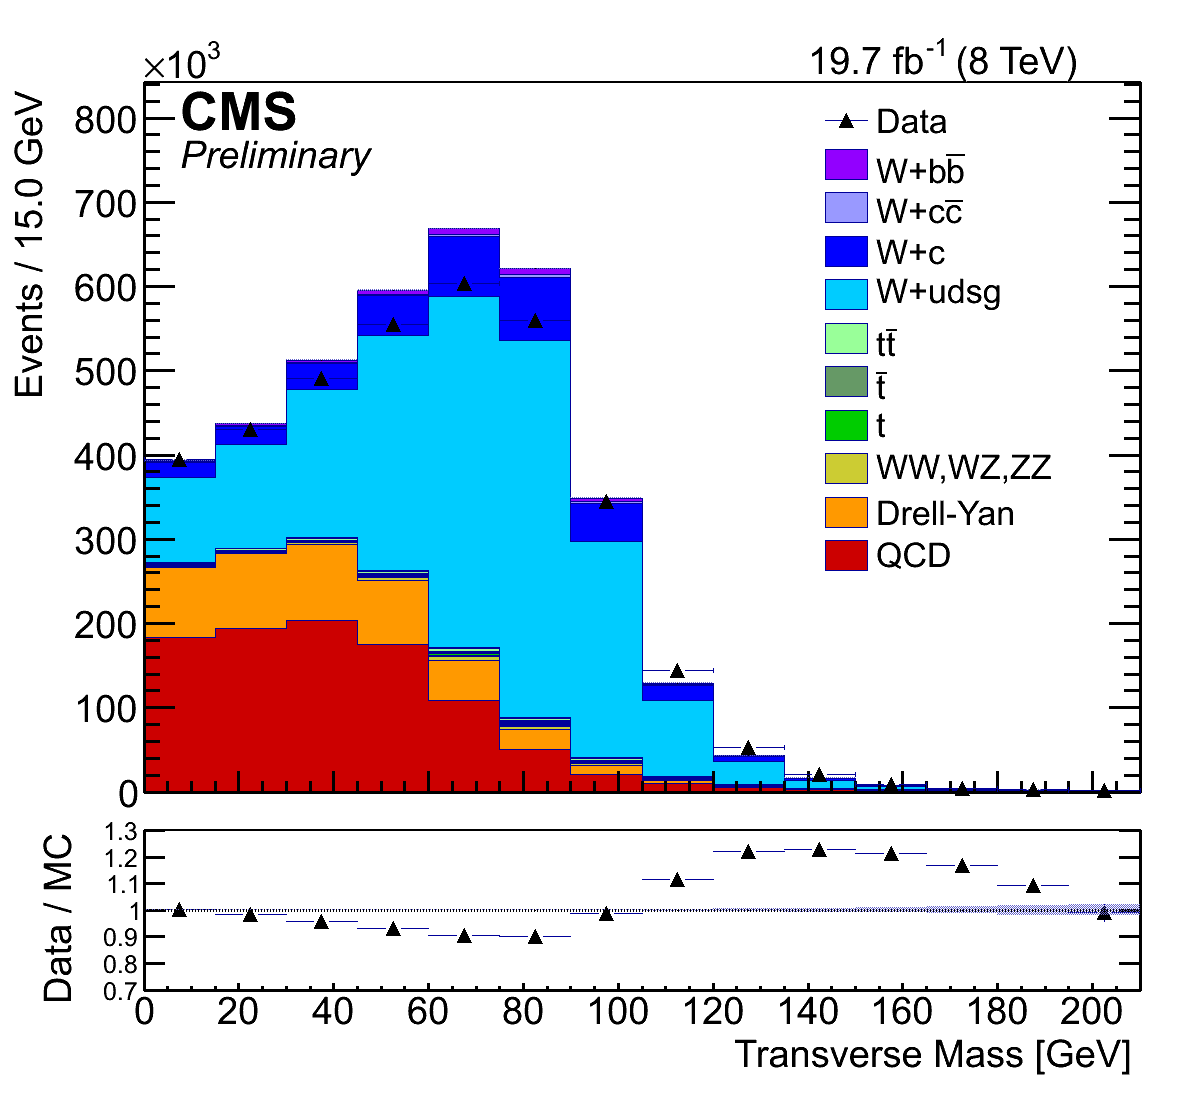
\includegraphics[width=0.4\textwidth]{/Users/rhombus/CMS/Thesis/thesis/pdfs/wbbxc/wjj/Histograms_wjj_mt_ele.png}
    \label{fig:wjj_plots}
\end{figure}

The true $\wc$ contribution in the signal region is minimal, 
and only possible due to mistaging of a second jet in
the event. However, the contribution of events
with one hard charm and one hard anti-charm originated by gluon 
splitting is not negligable and moreover these events have kinematics closely related 
to that of our signal. 

\subsection{Top backgrounds}
\label{section:topbackgrounds}

To validate the description of the $\ttbar$ contribution two 
 control regions are defined and referred to as multilepton 
 and multijet $\ttbar$ regions.
The selections for the multijet region are the same as 
 those for the $\wbb$ region except that additional jet
 activity is required by selecting events with at least
 three jets in the final state. 
Because of the loosening of the jet veto in this phase space,
 it is less sensative to the effects of jet energy scaling
 than the signal region (2\% in the \ttbar multijet phase space,
 6\% in the \wbb phase space.)
As can be seen in Figure \ref{fig:prefit_ttjjj},
 this control region is dominated by $\ttbar$, with $\ttbar$ accounting for
 80\% of the data yield.

\begin{figure}
      \caption[\ttbar-multijet control region for the \wbb measurement]
   {Distributions in the $\ttbar$ multijet control region are shown here in both channels.
       These raw distributions are made before any of the scaling outlined in Section \ref{subsec:wbb_analysisstrategy}.
       Left plots are in the muon decay channel and right
        plots are in the electron decay channel.
      }
      \center
 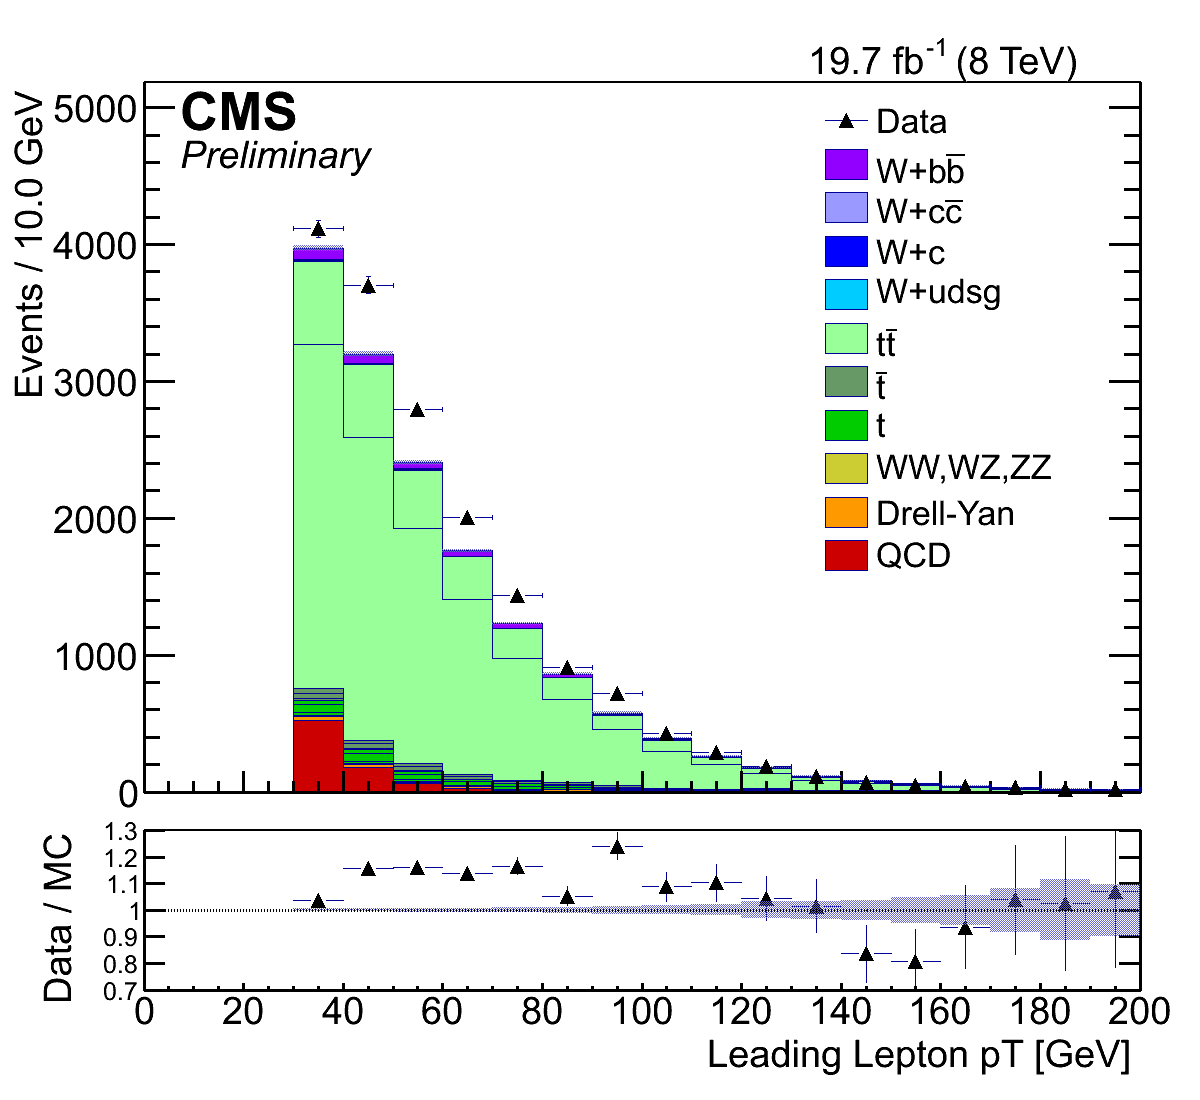
\includegraphics[width=0.4\textwidth]{/Users/rhombus/CMS/Thesis/thesis/pdfs/wbbxc/ttjjj/Histograms_ttjjj_goodLep_pt_mu.png}
 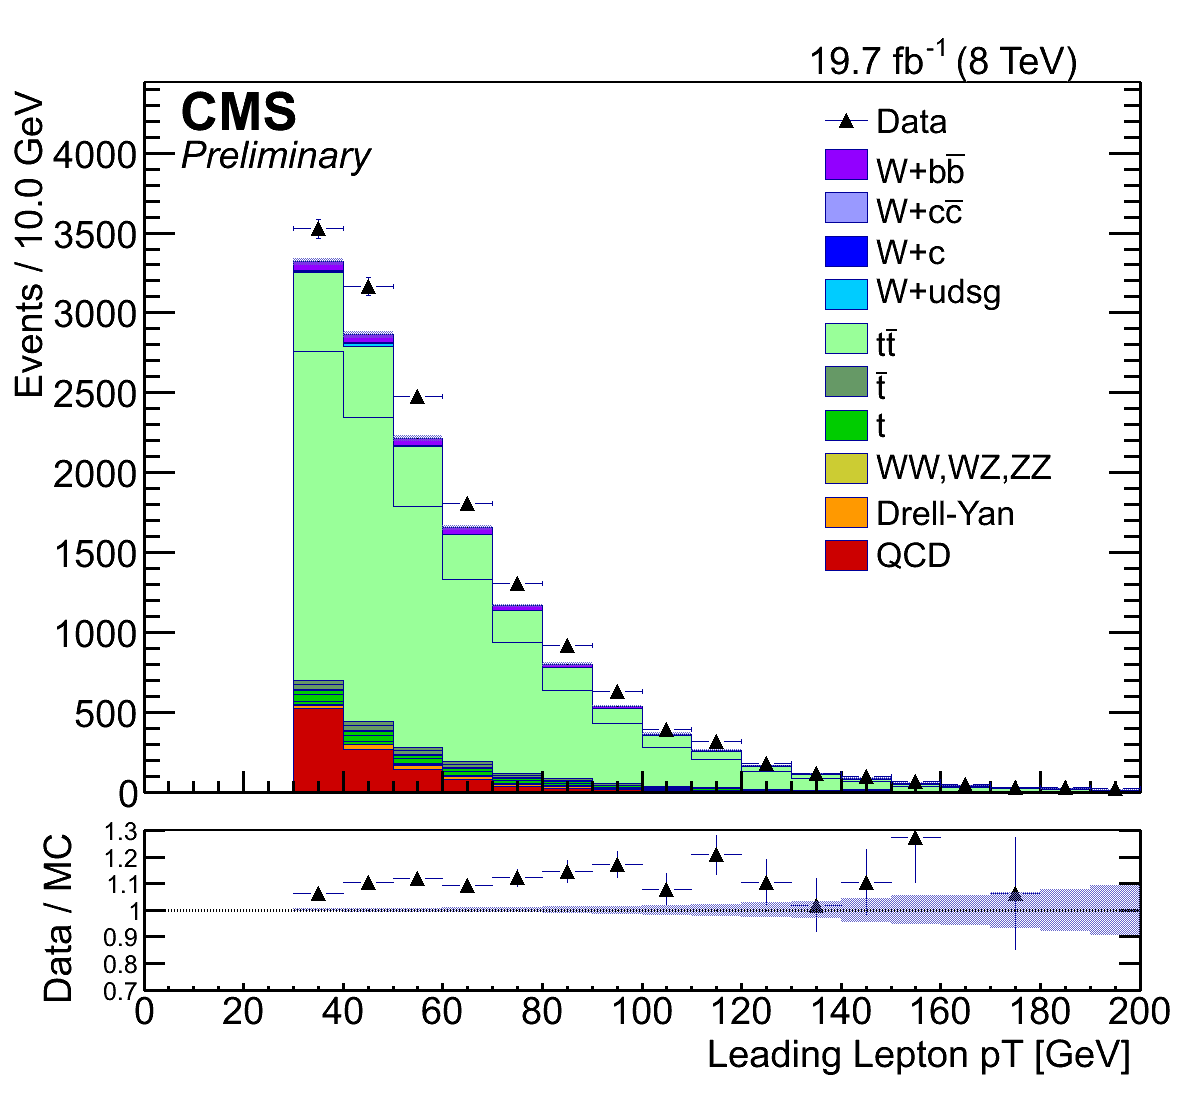
\includegraphics[width=0.4\textwidth]{/Users/rhombus/CMS/Thesis/thesis/pdfs/wbbxc/ttjjj/Histograms_ttjjj_goodLep_pt_ele.png}
 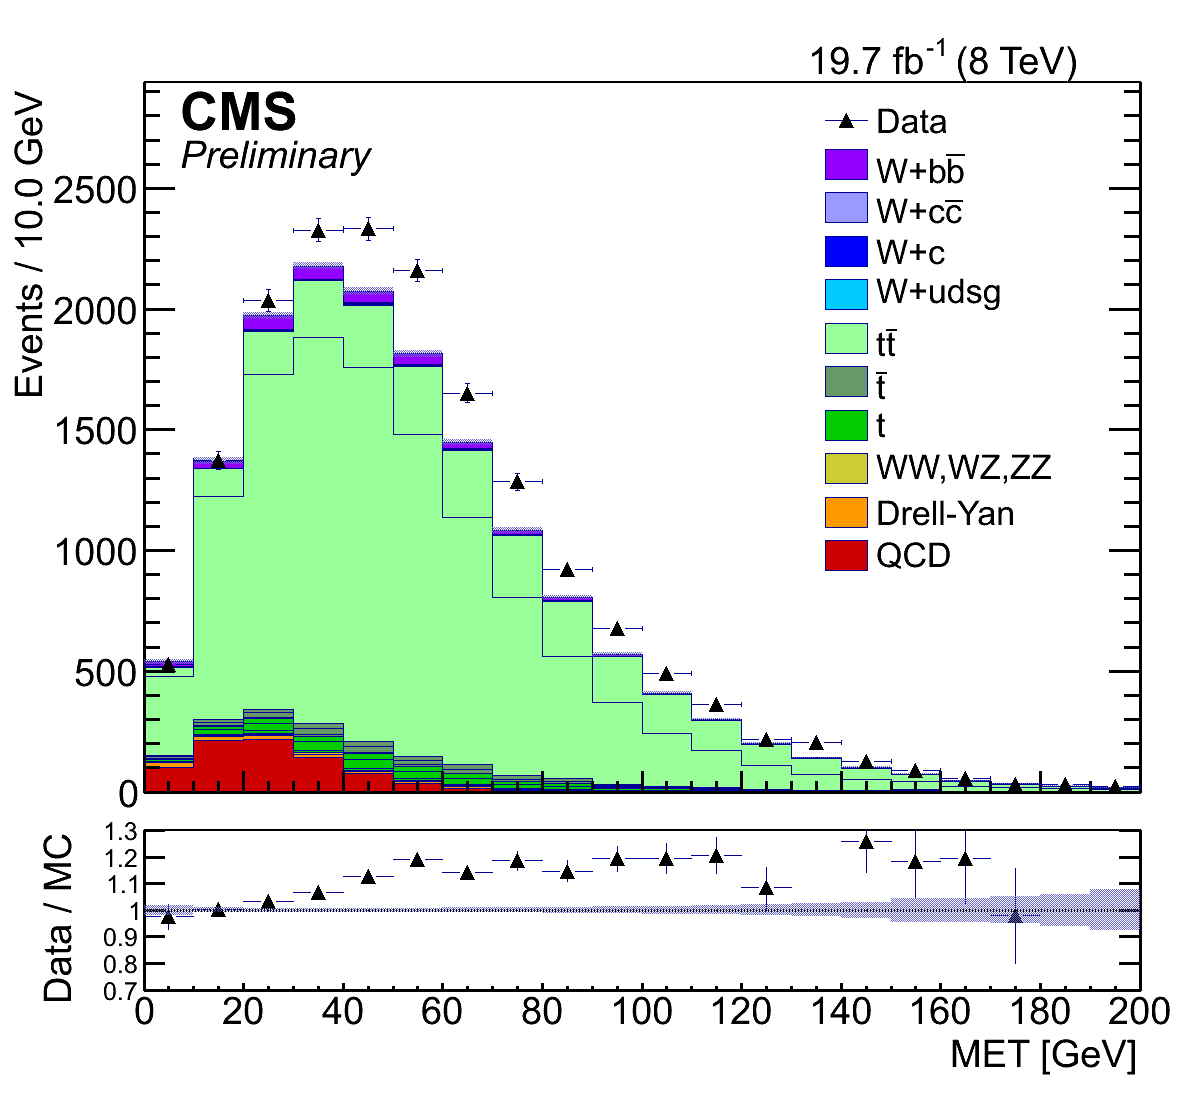
\includegraphics[width=0.4\textwidth]{/Users/rhombus/CMS/Thesis/thesis/pdfs/wbbxc/ttjjj/Histograms_ttjjj_met_mu.png}
 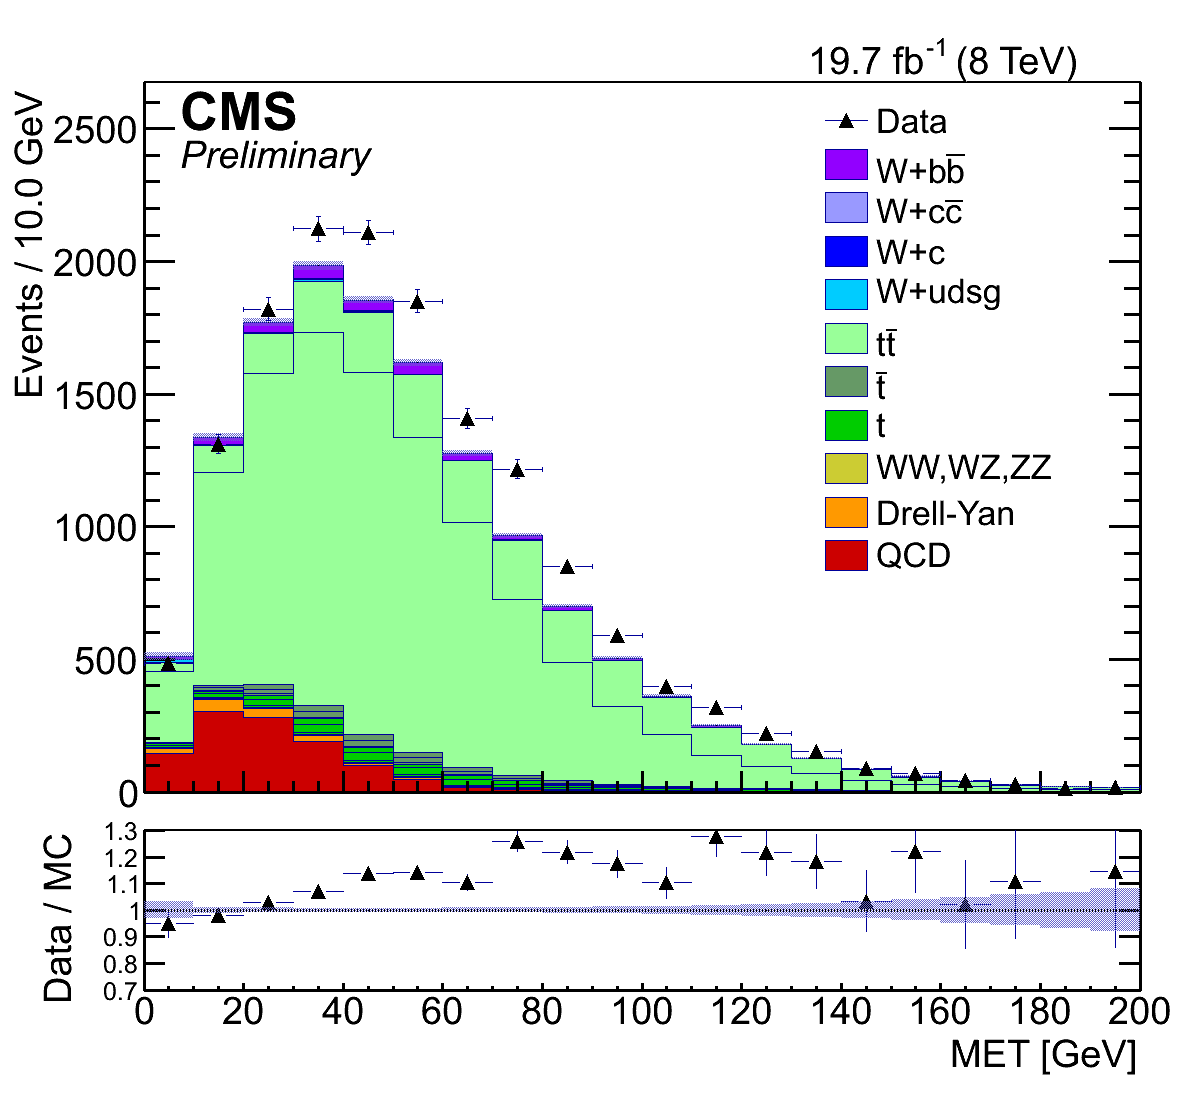
\includegraphics[width=0.4\textwidth]{/Users/rhombus/CMS/Thesis/thesis/pdfs/wbbxc/ttjjj/Histograms_ttjjj_met_ele.png}
 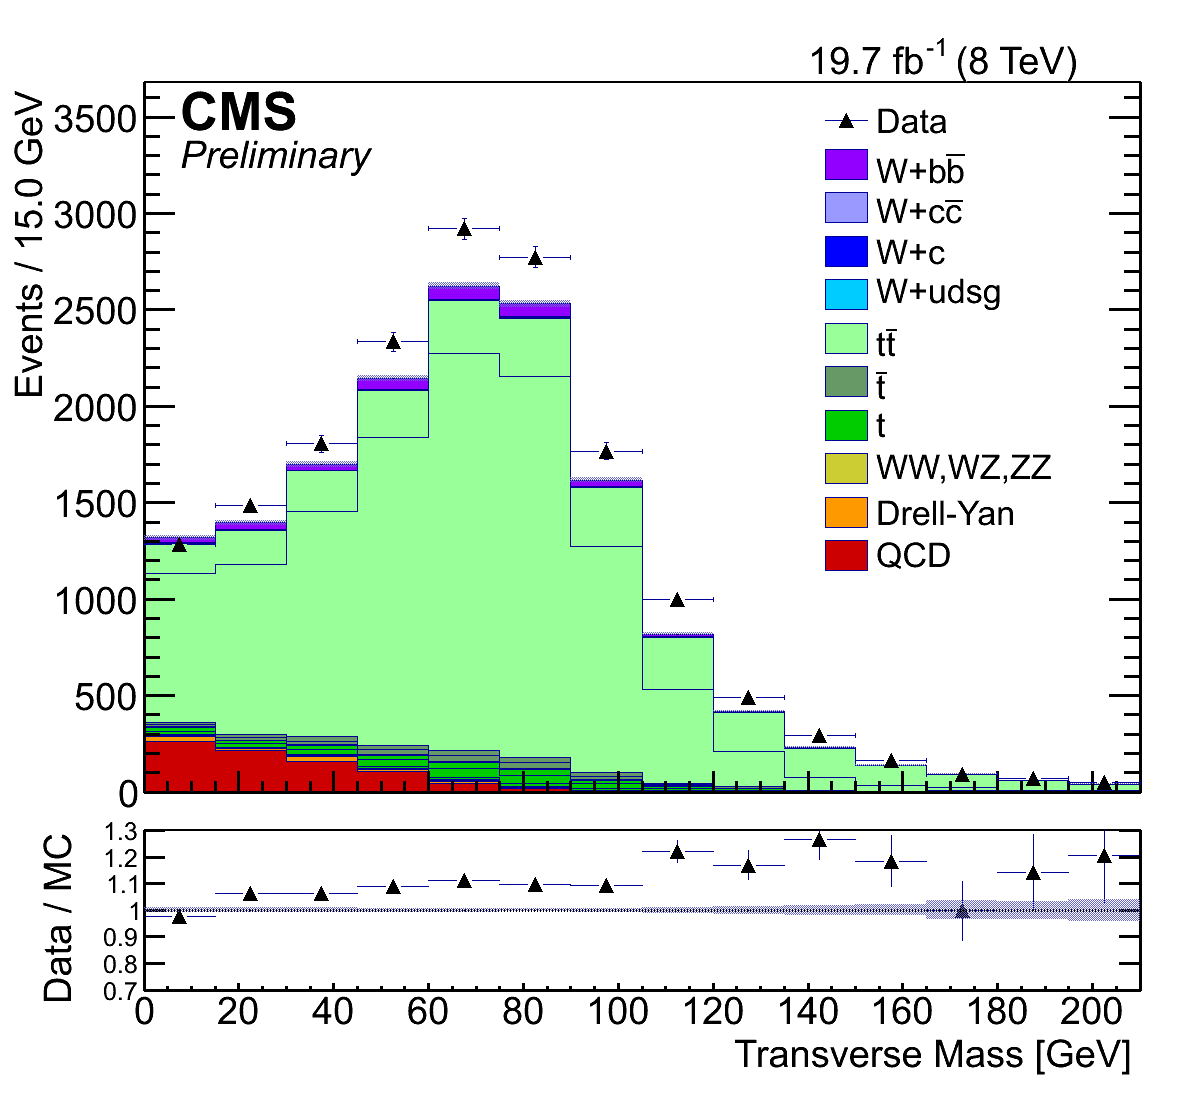
\includegraphics[width=0.4\textwidth]{/Users/rhombus/CMS/Thesis/thesis/pdfs/wbbxc/ttjjj/Histograms_ttjjj_mt_mu.png}
 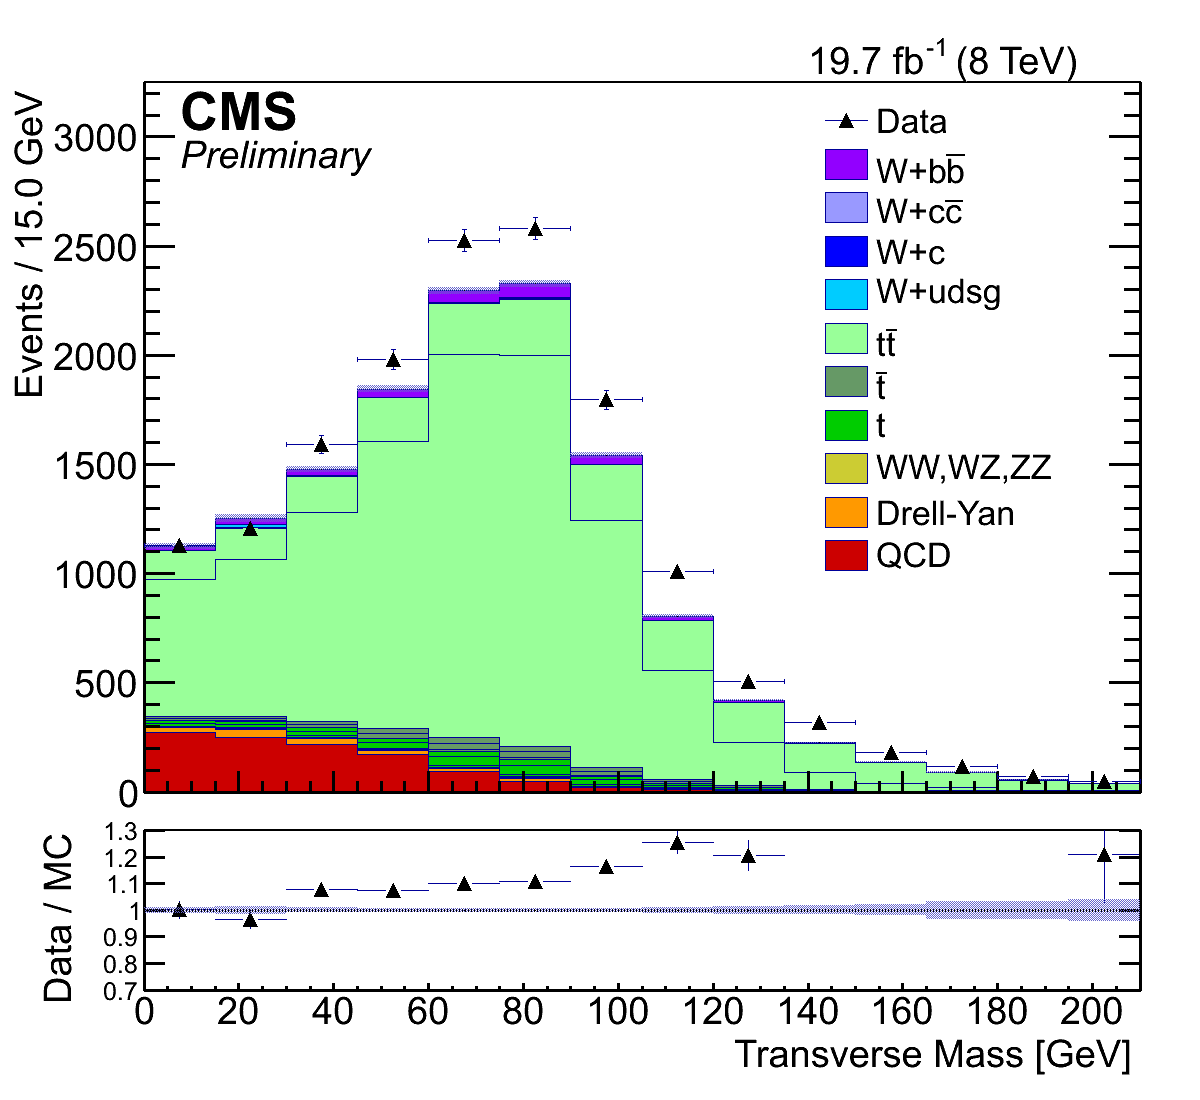
\includegraphics[width=0.4\textwidth]{/Users/rhombus/CMS/Thesis/thesis/pdfs/wbbxc/ttjjj/Histograms_ttjjj_mt_ele.png}
      \label{fig:prefit_ttjjj}
\end{figure}


The selections for the multilepton region differ from those for
 the $\wbb$ region in that exactly two well-isolated
 opposite-flavor leptons are required. 
Figure \ref{fig:prefit_ttme} shows representative distributions
 in this phase space where $\ttbar$ accounts for over
 95\% of the simulated samples.
%A detailed study of this phase space is presented in 
% Appendix \ref{sec:ttcrosscheck}.

\begin{figure}
      \caption[\ttbar-multilepton control region for the \wbb measurement]
    {Distributions in the $\ttbar$ multilepton control region are shown here in both channels.
       These raw distributions are made before any of the scaling outlined in Section \ref{subsec:wbb_analysisstrategy}.
       Left plots are in the muon decay channel and right
        plots are in the electron decay channel.
      }
      \center
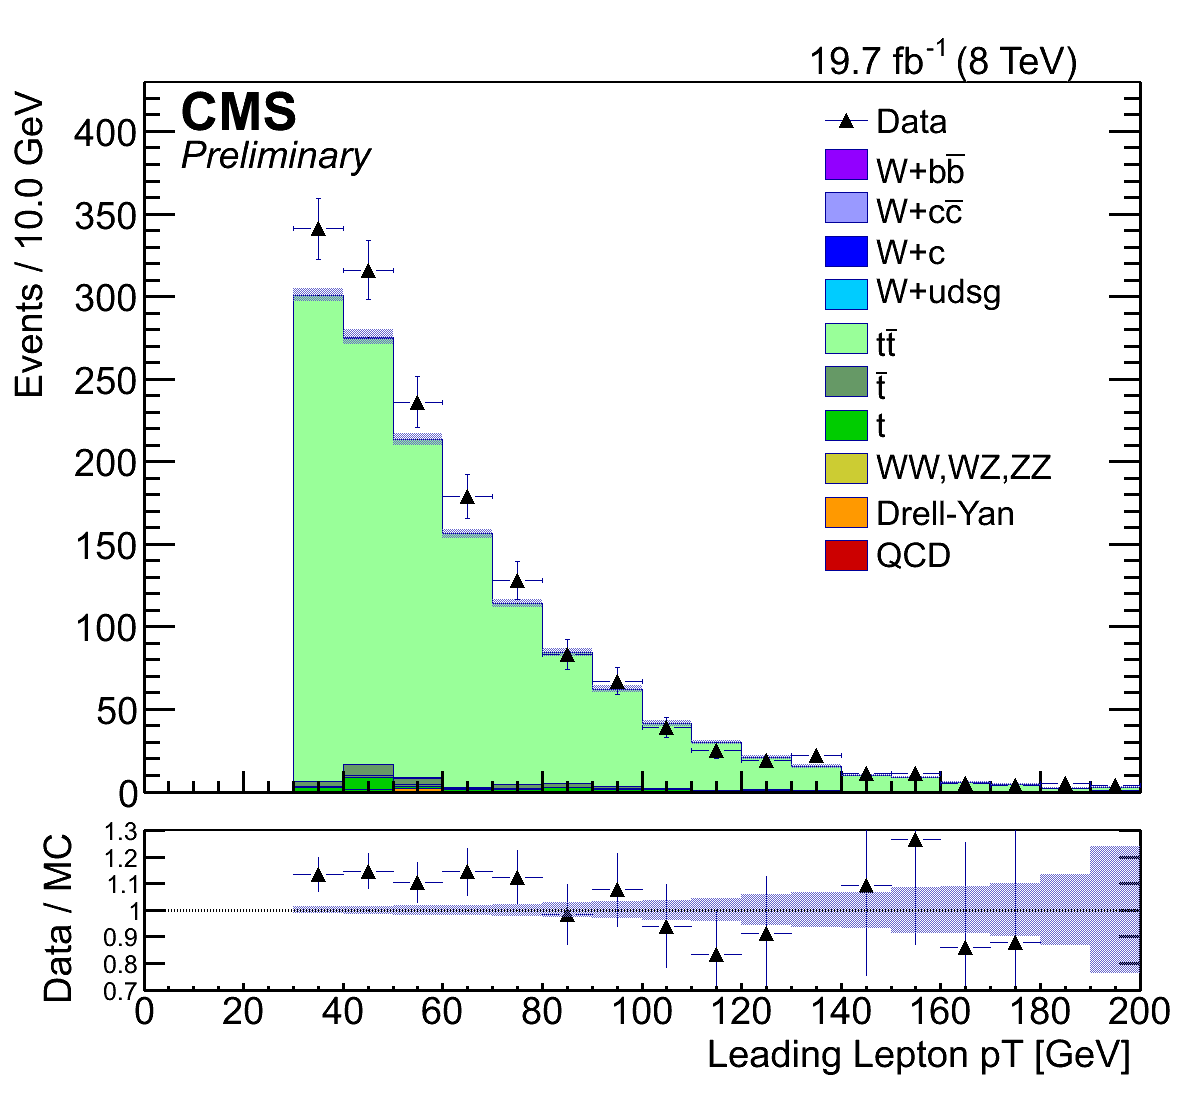
\includegraphics[width=0.4\textwidth]{/Users/rhombus/CMS/Thesis/thesis/pdfs/wbbxc/ttme/Histograms_ttme_goodLep_pt_mu.png}
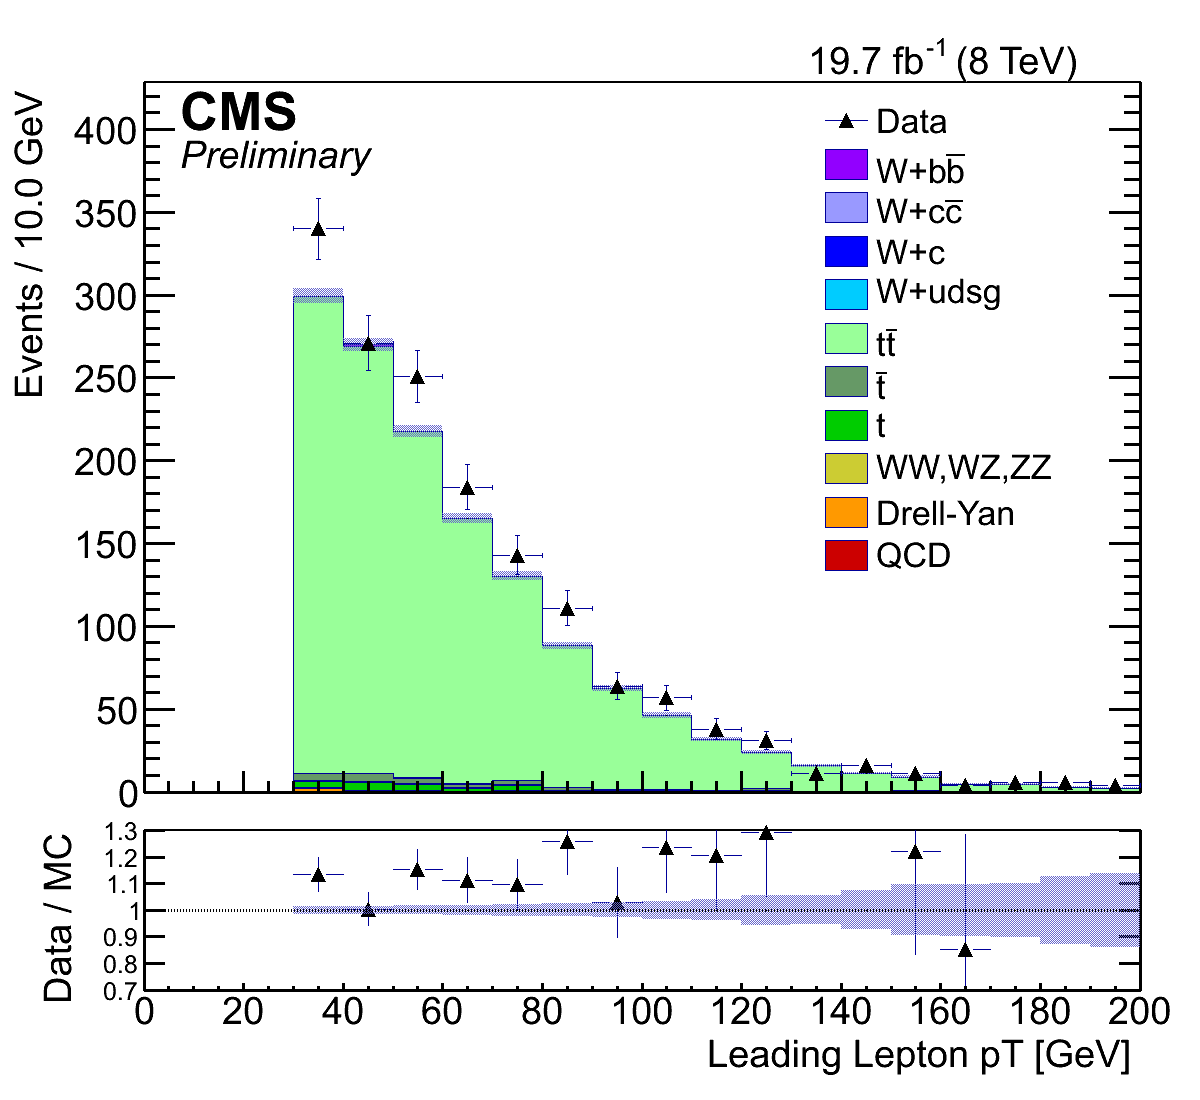
\includegraphics[width=0.4\textwidth]{/Users/rhombus/CMS/Thesis/thesis/pdfs/wbbxc/ttme/Histograms_ttme_goodLep_pt_ele.png}
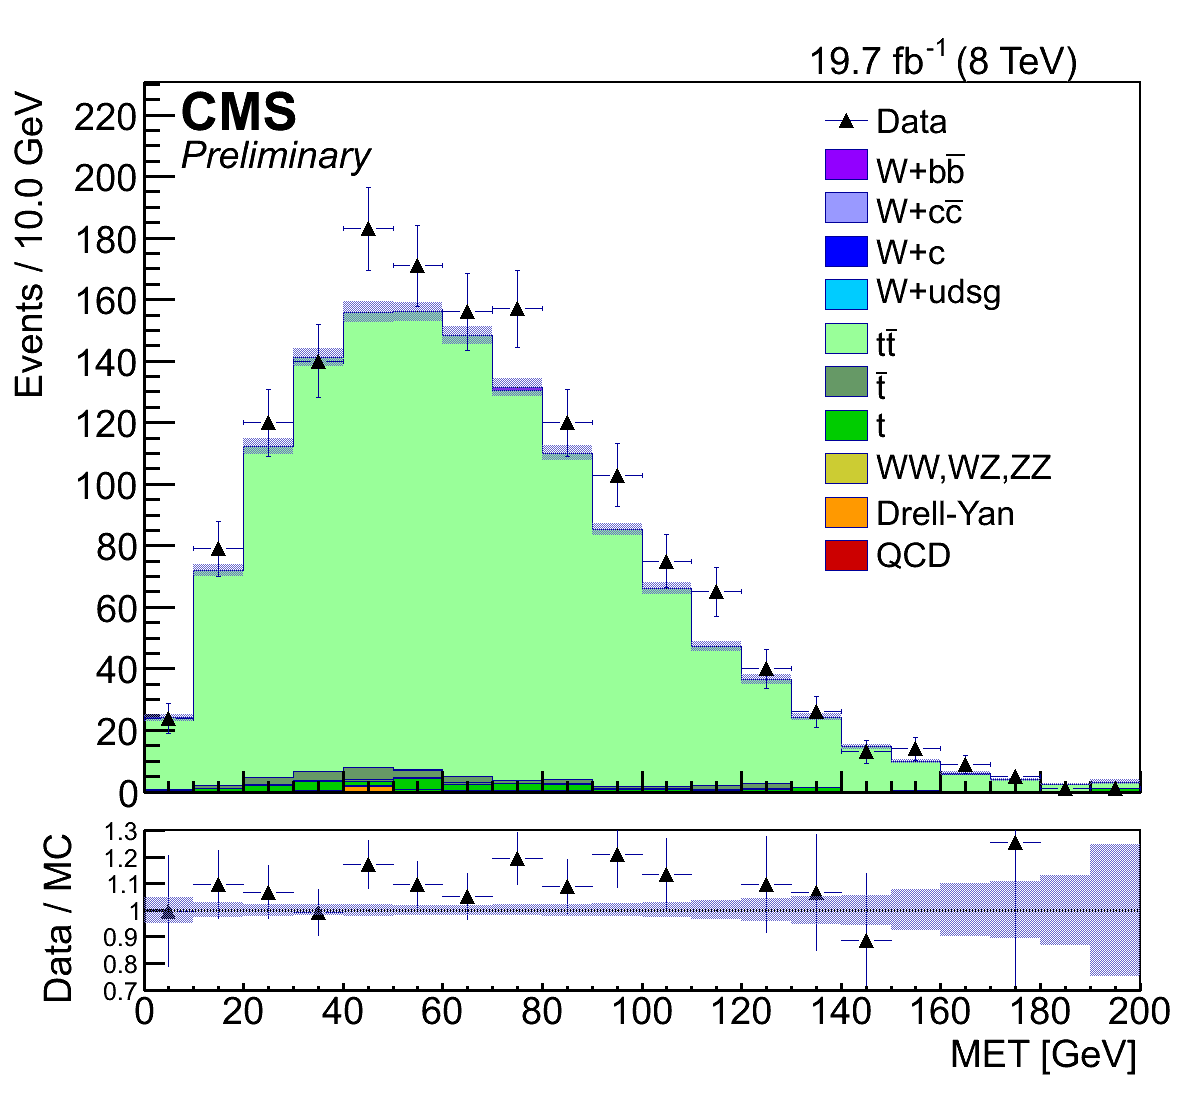
\includegraphics[width=0.4\textwidth]{/Users/rhombus/CMS/Thesis/thesis/pdfs/wbbxc/ttme/Histograms_ttme_met_mu.png}
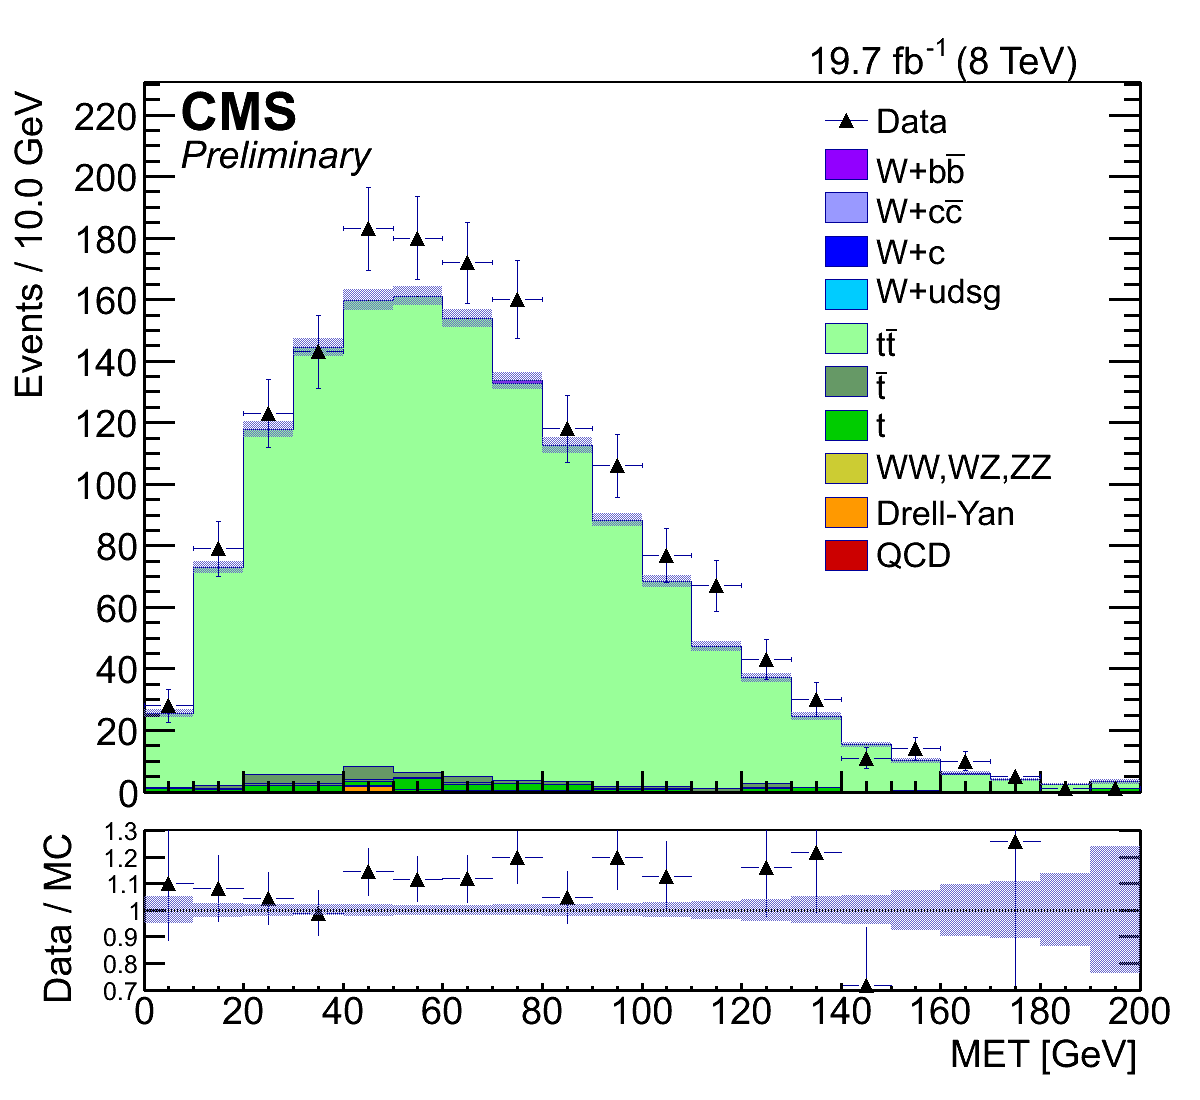
\includegraphics[width=0.4\textwidth]{/Users/rhombus/CMS/Thesis/thesis/pdfs/wbbxc/ttme/Histograms_ttme_met_ele.png}
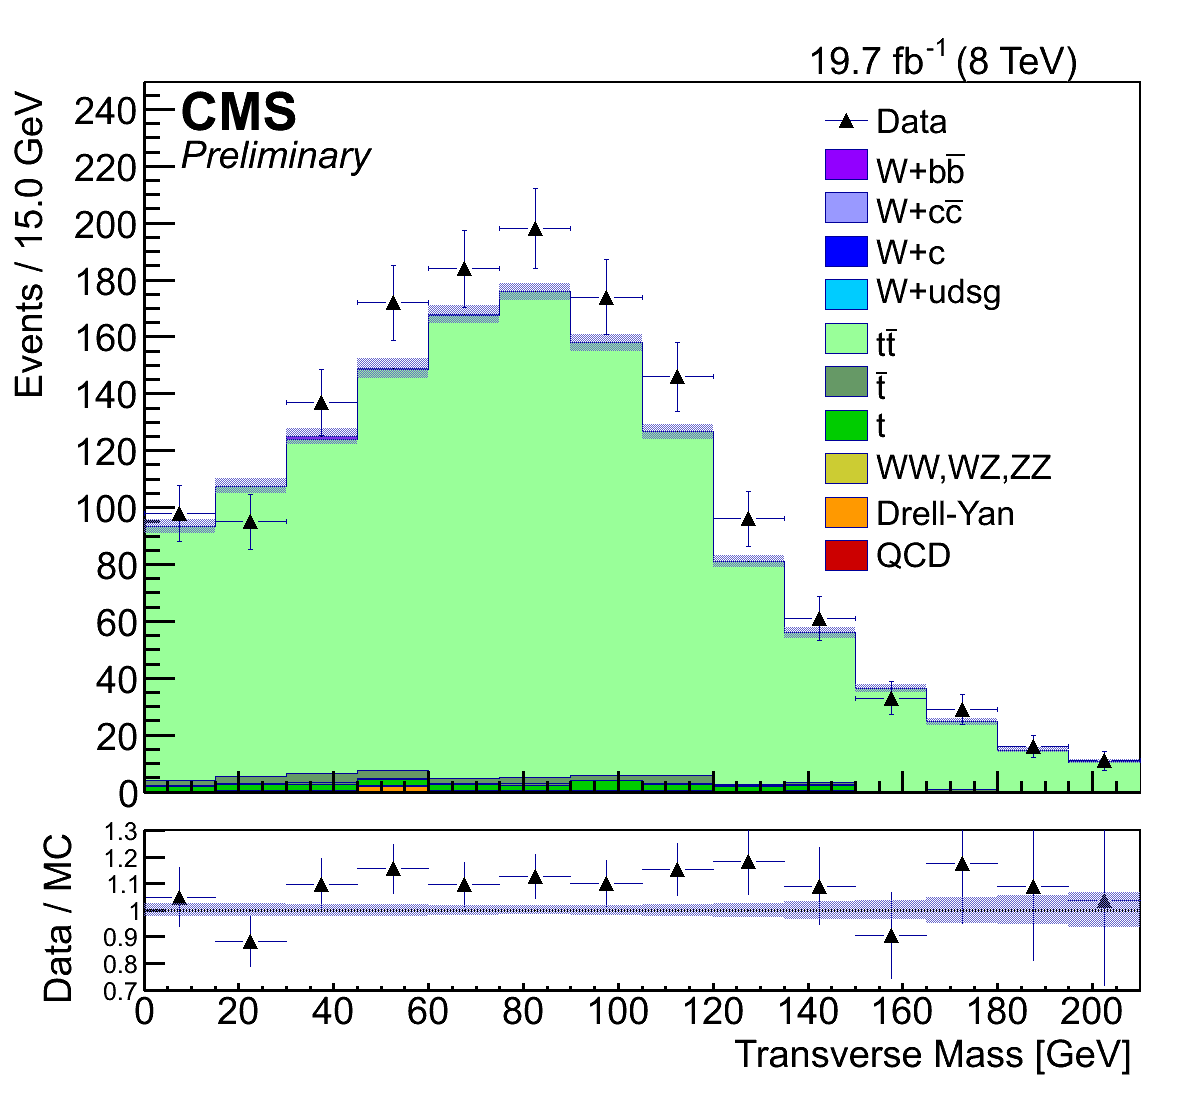
\includegraphics[width=0.4\textwidth]{/Users/rhombus/CMS/Thesis/thesis/pdfs/wbbxc/ttme/Histograms_ttme_mt_mu.png}
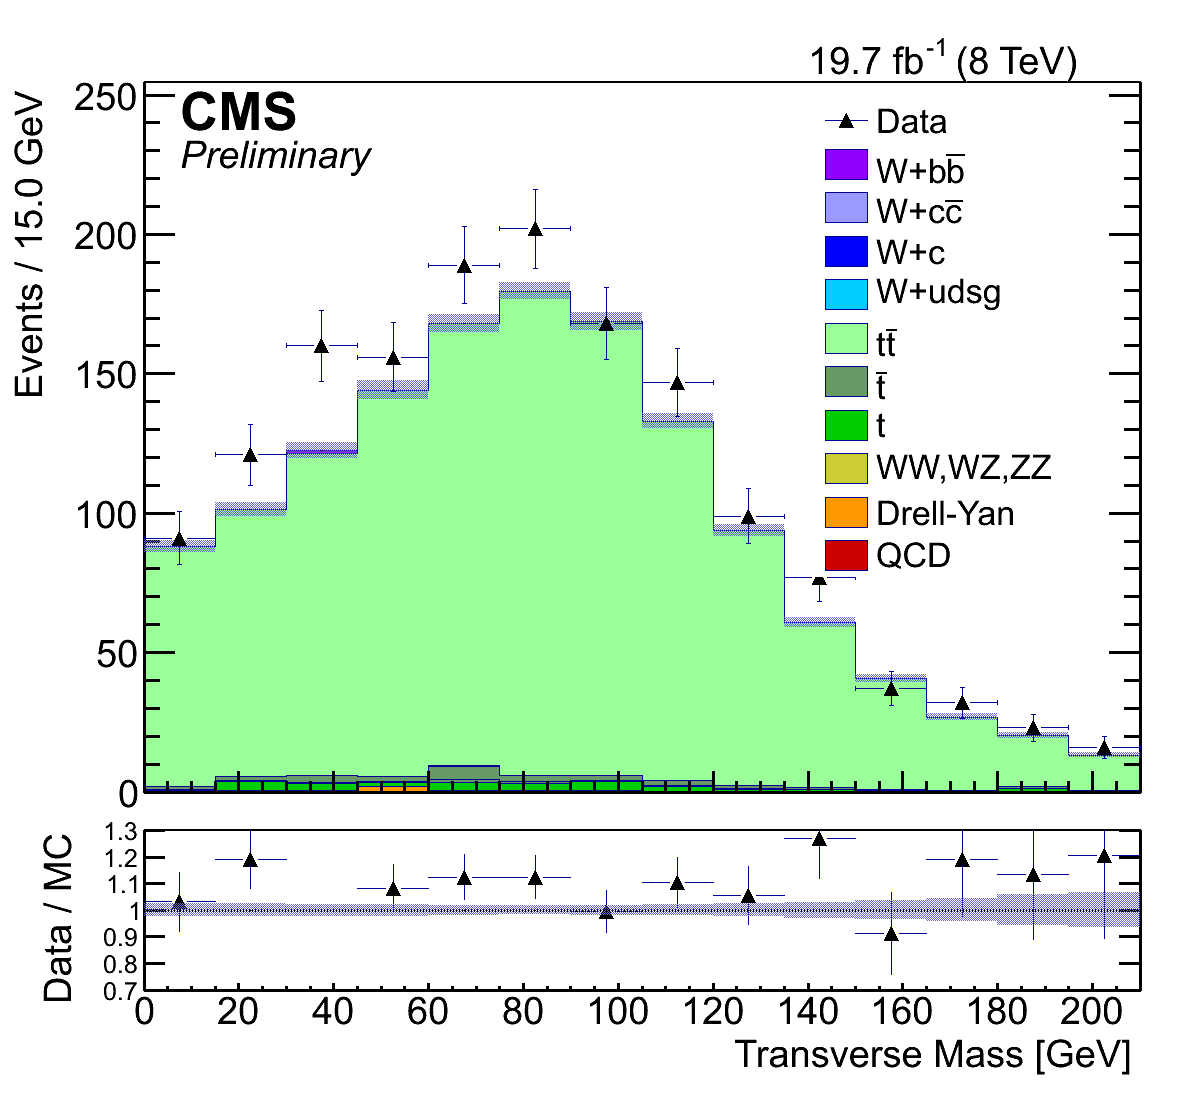
\includegraphics[width=0.4\textwidth]{/Users/rhombus/CMS/Thesis/thesis/pdfs/wbbxc/ttme/Histograms_ttme_mt_ele.png}
      \label{fig:prefit_ttme}
\end{figure}

The single top control region is defined by the signal selection requirements
 without the third and forward jet vetos, and
 with the leading jet required to be central
 ($|\eta|<2.4$) and tightly b-tagged,
 while the subleading jet has no $b$ requirement and must fall within
 $2.4<|\eta|<5.0$.
As illustrated in Figure \ref{fig:prefit_stt}, there are many 
 backgrounds contaminating the purity of this phase space,
 but agreement between data and simulation is on the order of 5-10\%.
\begin{figure}
      \caption[Single-top control region for the \wbb measurement]{The single top control region is defined by one b-tagged central jet and one forward jet.
      Shown above are distributions in the single top control region.
       Left plots are in the muon decay channel and right
        plots are in the electron decay channel.
      }
      \center
 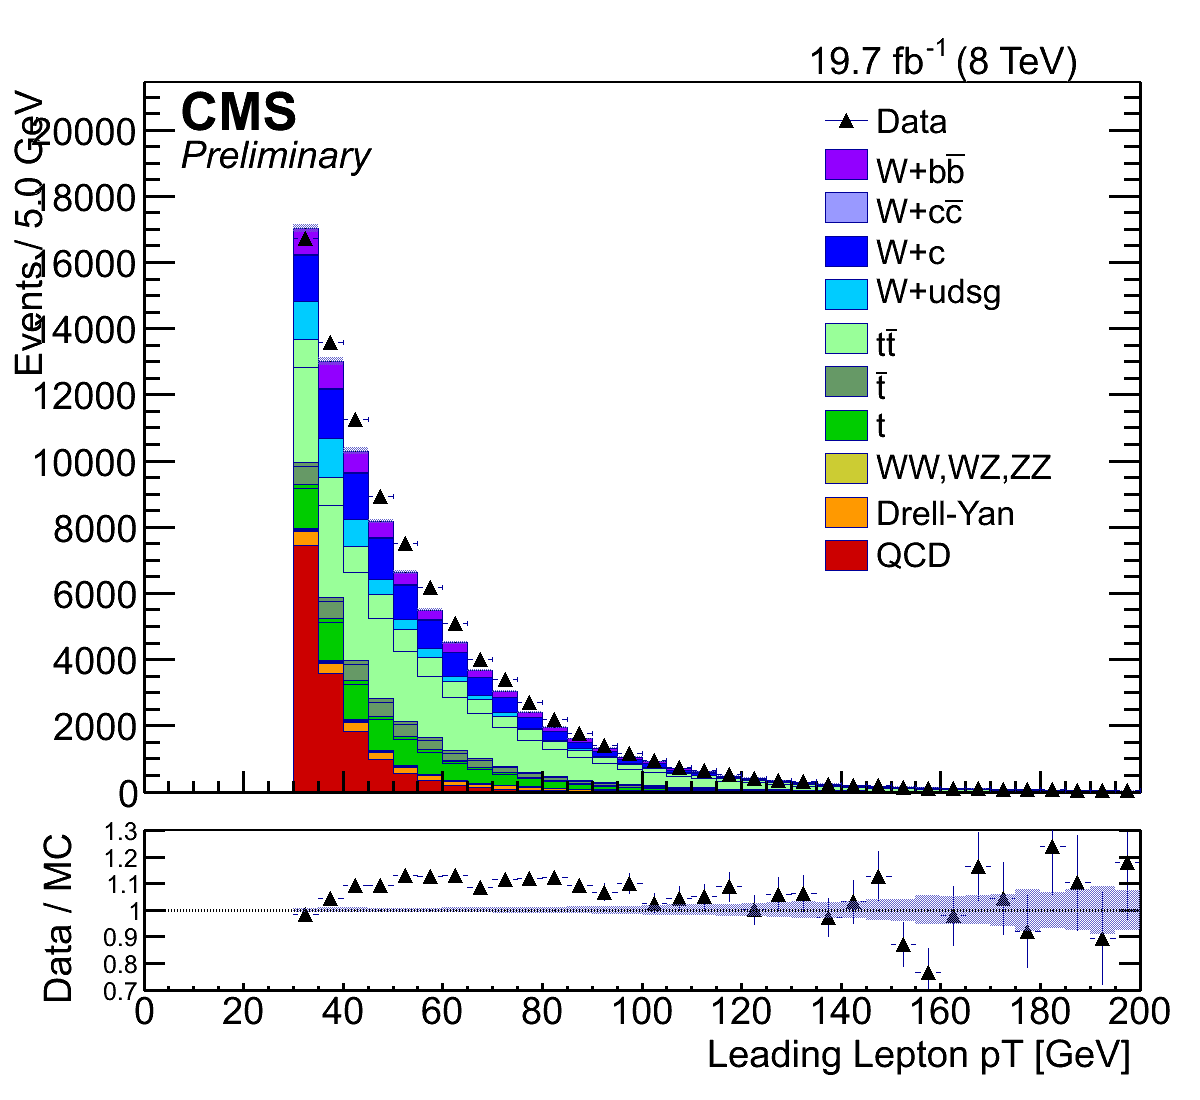
\includegraphics[width=0.4\textwidth]{/Users/rhombus/CMS/Thesis/thesis/pdfs/wbbxc/stt/Histograms_stt_goodLep_pt_mu.png}
 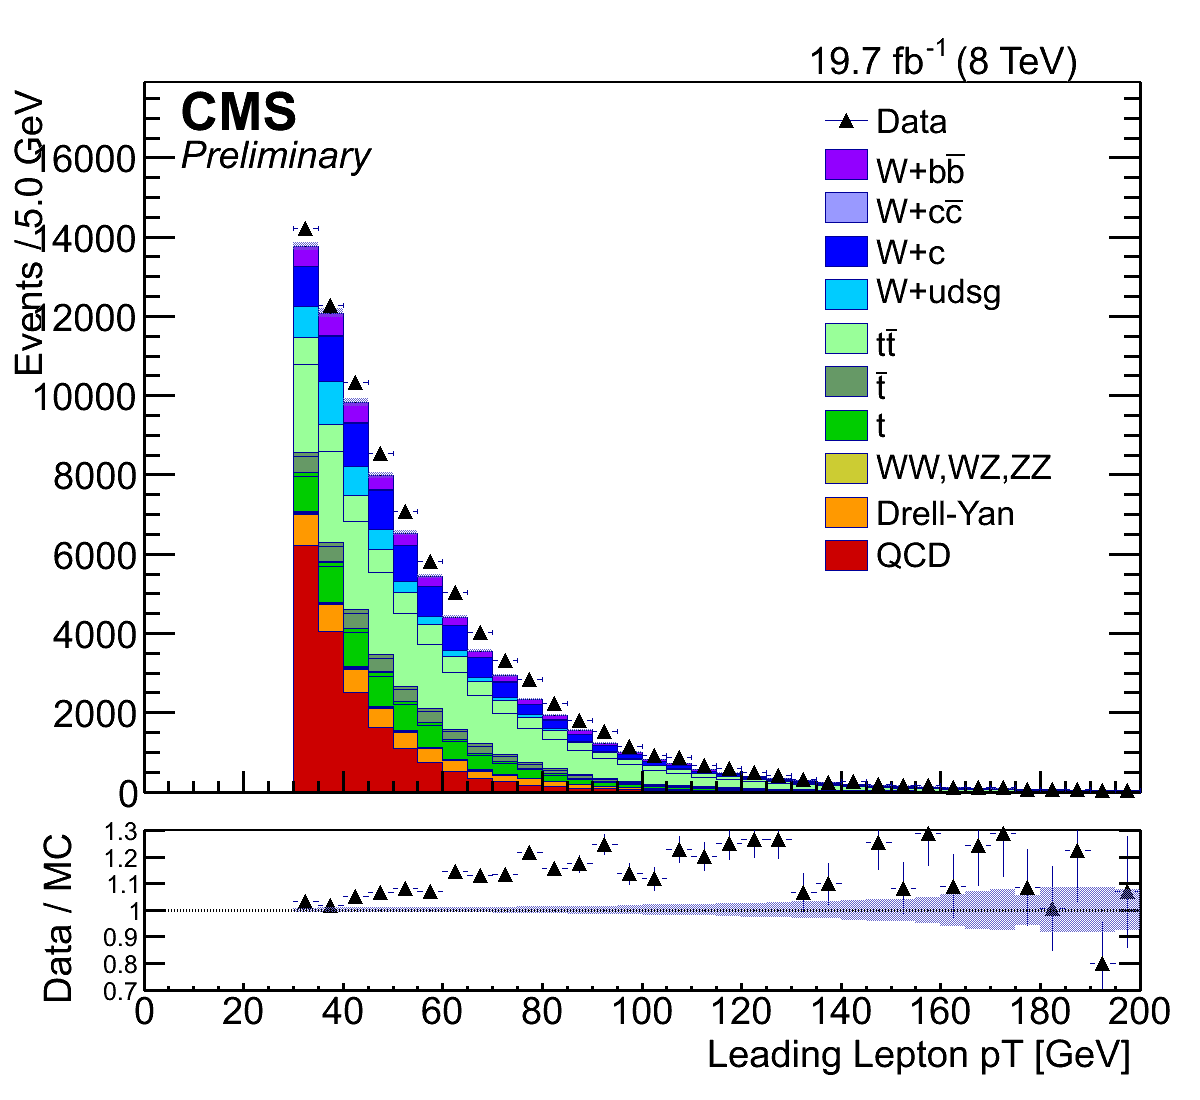
\includegraphics[width=0.4\textwidth]{/Users/rhombus/CMS/Thesis/thesis/pdfs/wbbxc/stt/Histograms_stt_goodLep_pt_ele.png}
 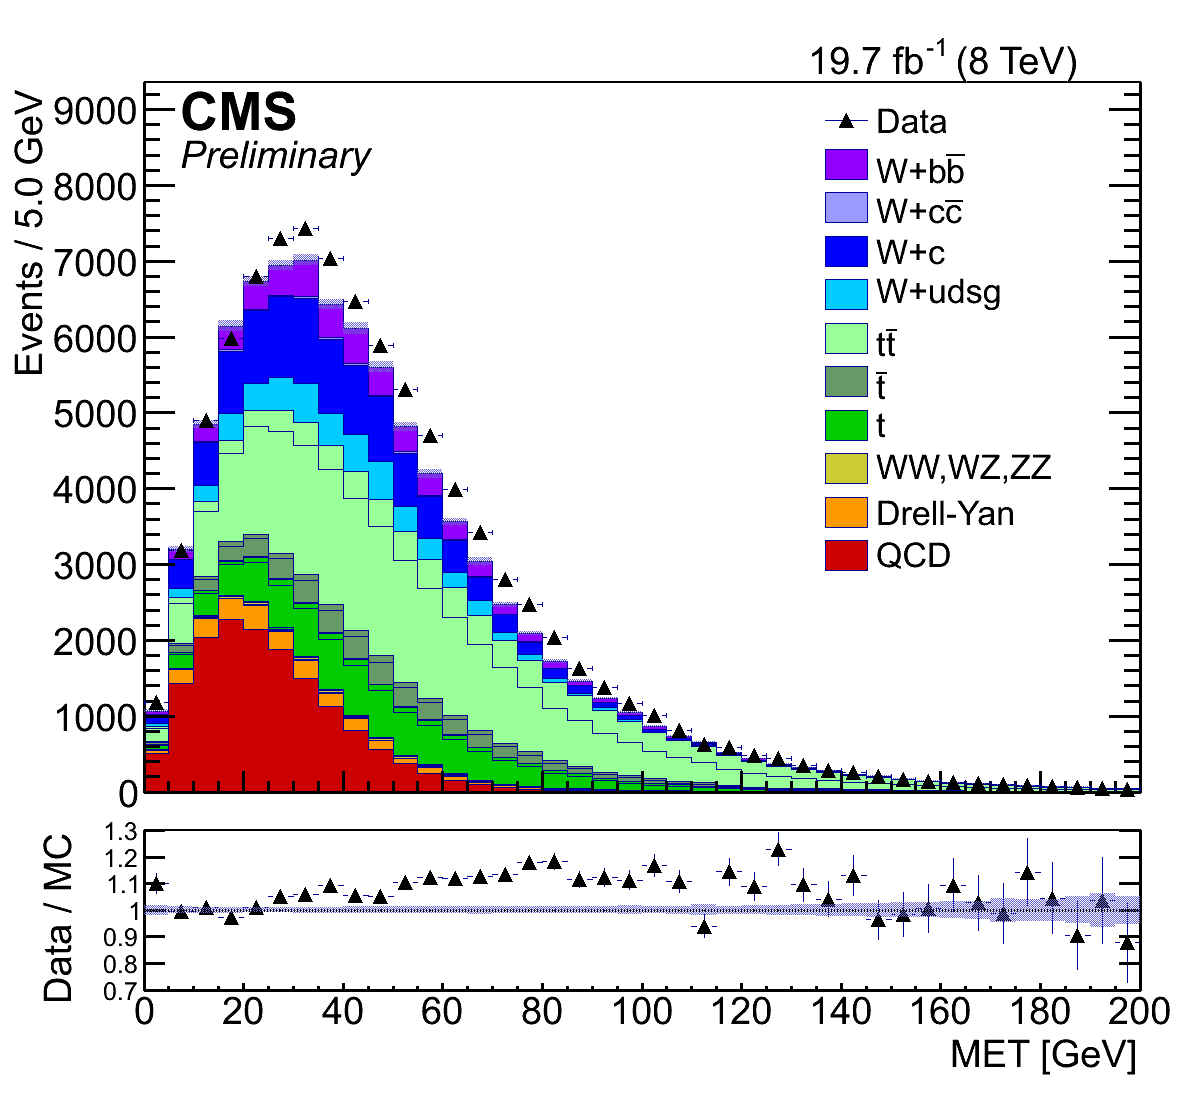
\includegraphics[width=0.4\textwidth]{/Users/rhombus/CMS/Thesis/thesis/pdfs/wbbxc/stt/Histograms_stt_met_mu.png}
 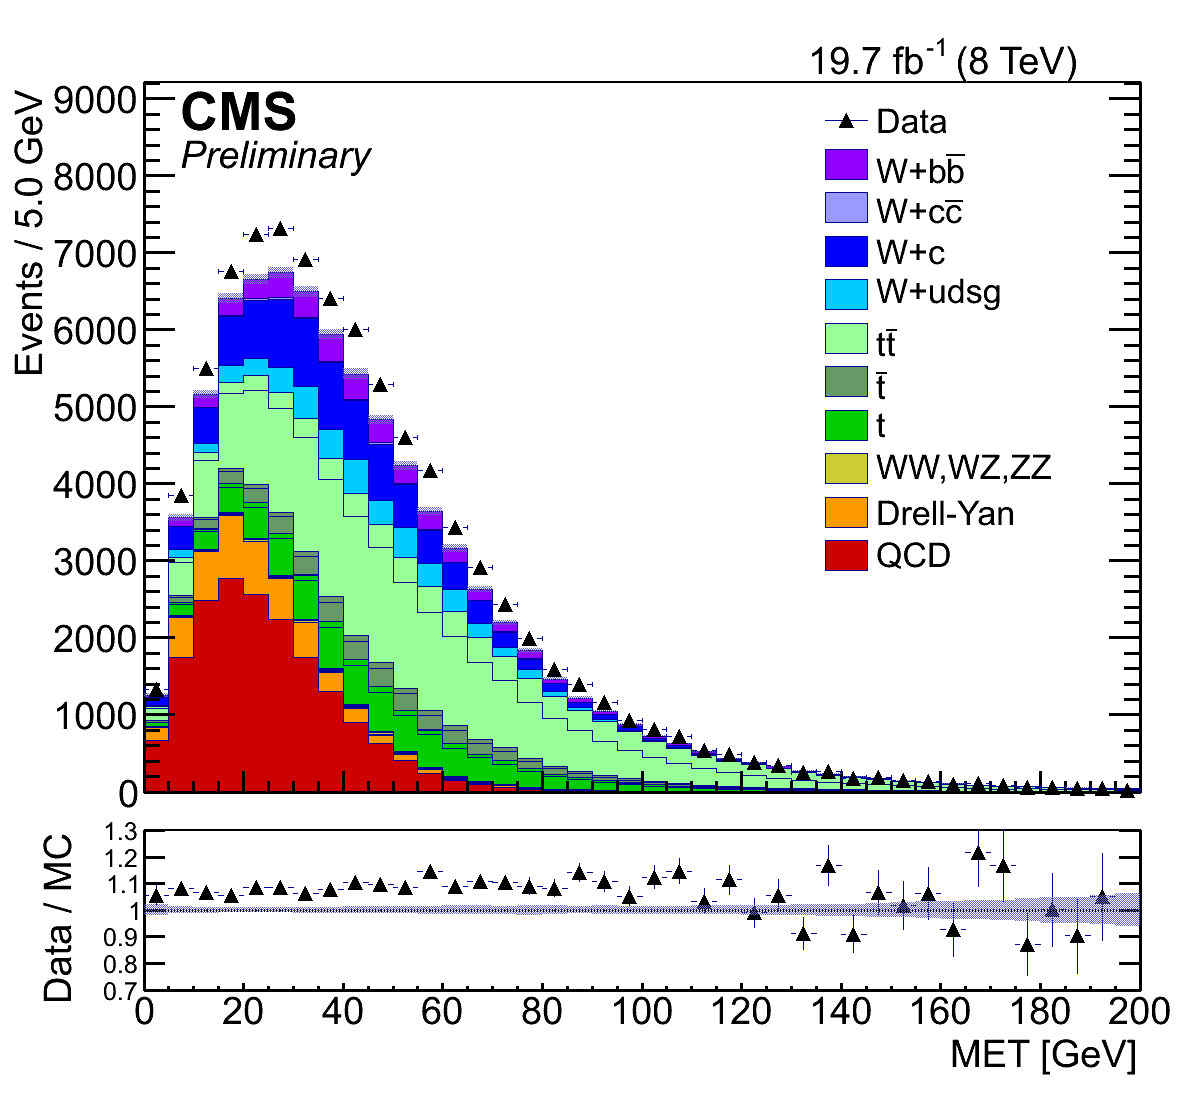
\includegraphics[width=0.4\textwidth]{/Users/rhombus/CMS/Thesis/thesis/pdfs/wbbxc/stt/Histograms_stt_met_ele.png}
 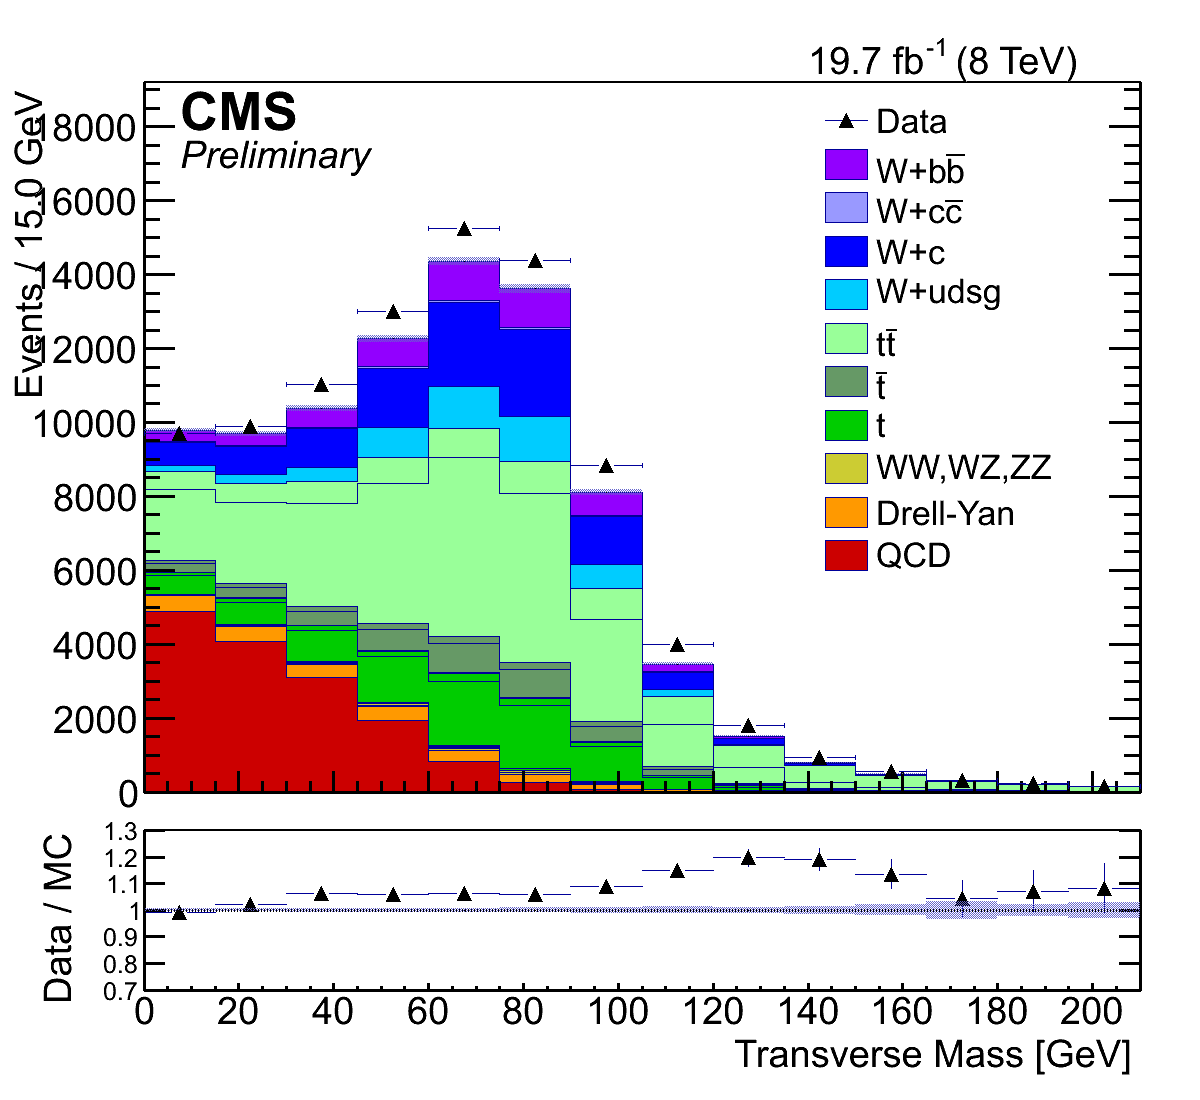
\includegraphics[width=0.4\textwidth]{/Users/rhombus/CMS/Thesis/thesis/pdfs/wbbxc/stt/Histograms_stt_mt_mu.png}
 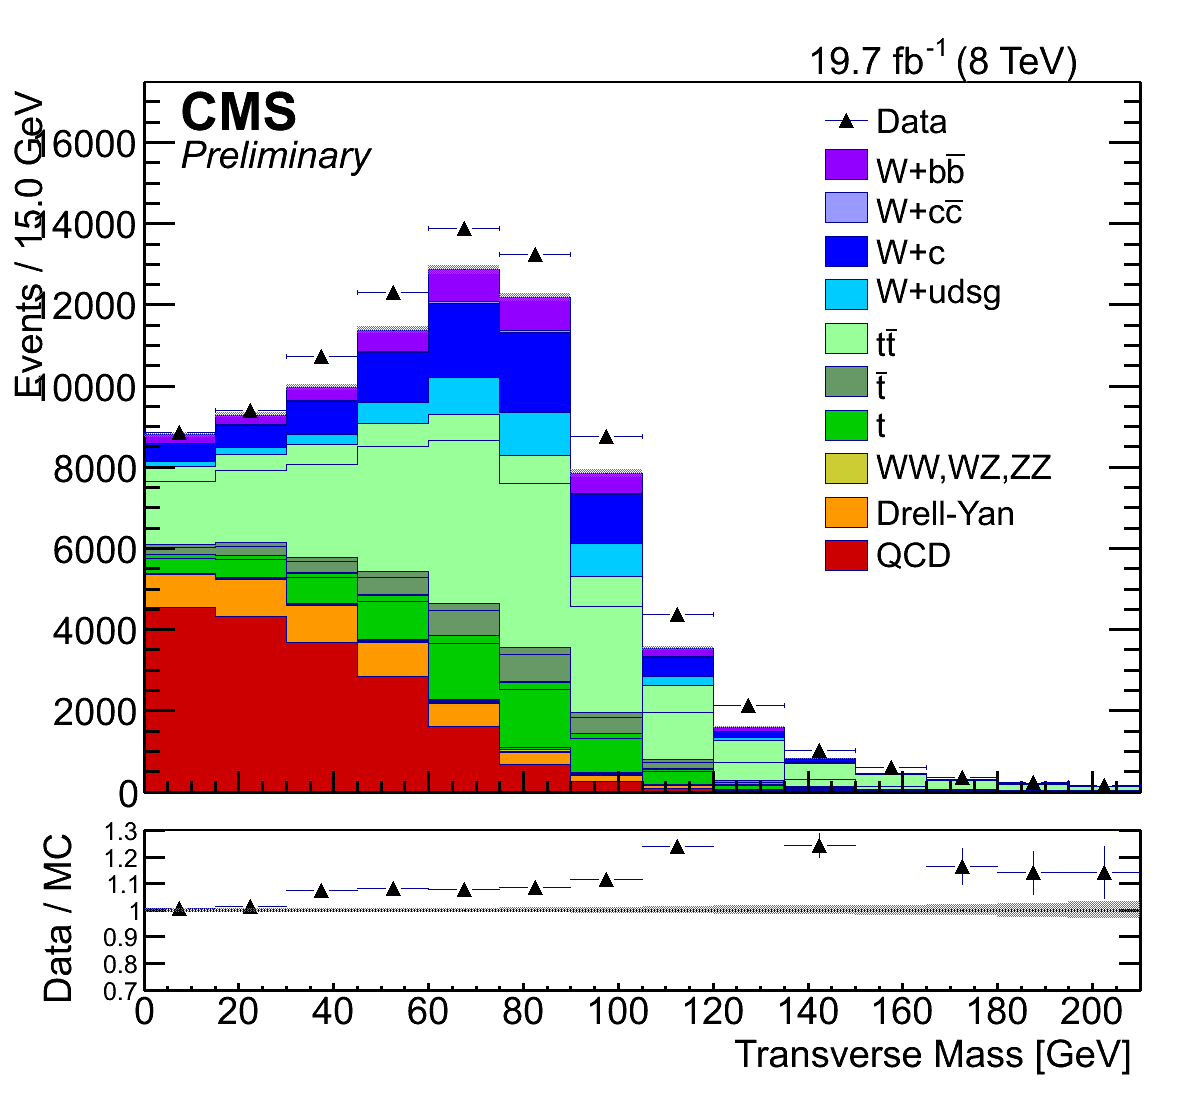
\includegraphics[width=0.4\textwidth]{/Users/rhombus/CMS/Thesis/thesis/pdfs/wbbxc/stt/Histograms_stt_mt_ele.png}
      \label{fig:prefit_stt}
\end{figure}


\subsection{\zll backgrounds}

The Drell-Yan backround is validated in a control region where the $\wbb$
 selection requirements are applied, but the lepton veto 
 is inverted, requiring two isolated, same-flavor leptons 
 and the $\mt$ requirement is dropped.
This is referred to as the $\zbb$ region and distributions
 of the mass and transverse momentum of the dilepton pair is
 shown in Figure \ref{fig:prefit_dybb}.
Contamination from \ttbar is evident. 
A cleaner Drell-Yan phase space is found by requiring exactly two jets
 but placing no b tag requirement and is referred to as $\zjj$.
Figure \ref{fig:prefit_dyjj} shows the same distributions as
 Figure \ref{fig:prefit_dybb} in this phase space.
%More cross checks on Drell-Yan are shown in Appendix \ref{sec:dycrosscheck}.

\begin{figure}
      \caption[\zbb control region for the \wbb analysis]{ Above are distributions of the mass and
        transverse momentum of the dilepton pair in the
        $\zbb$ phase space.
       Left plots are in the muon decay channel and right
        plots are in the electron decay channel.
      }
      \center
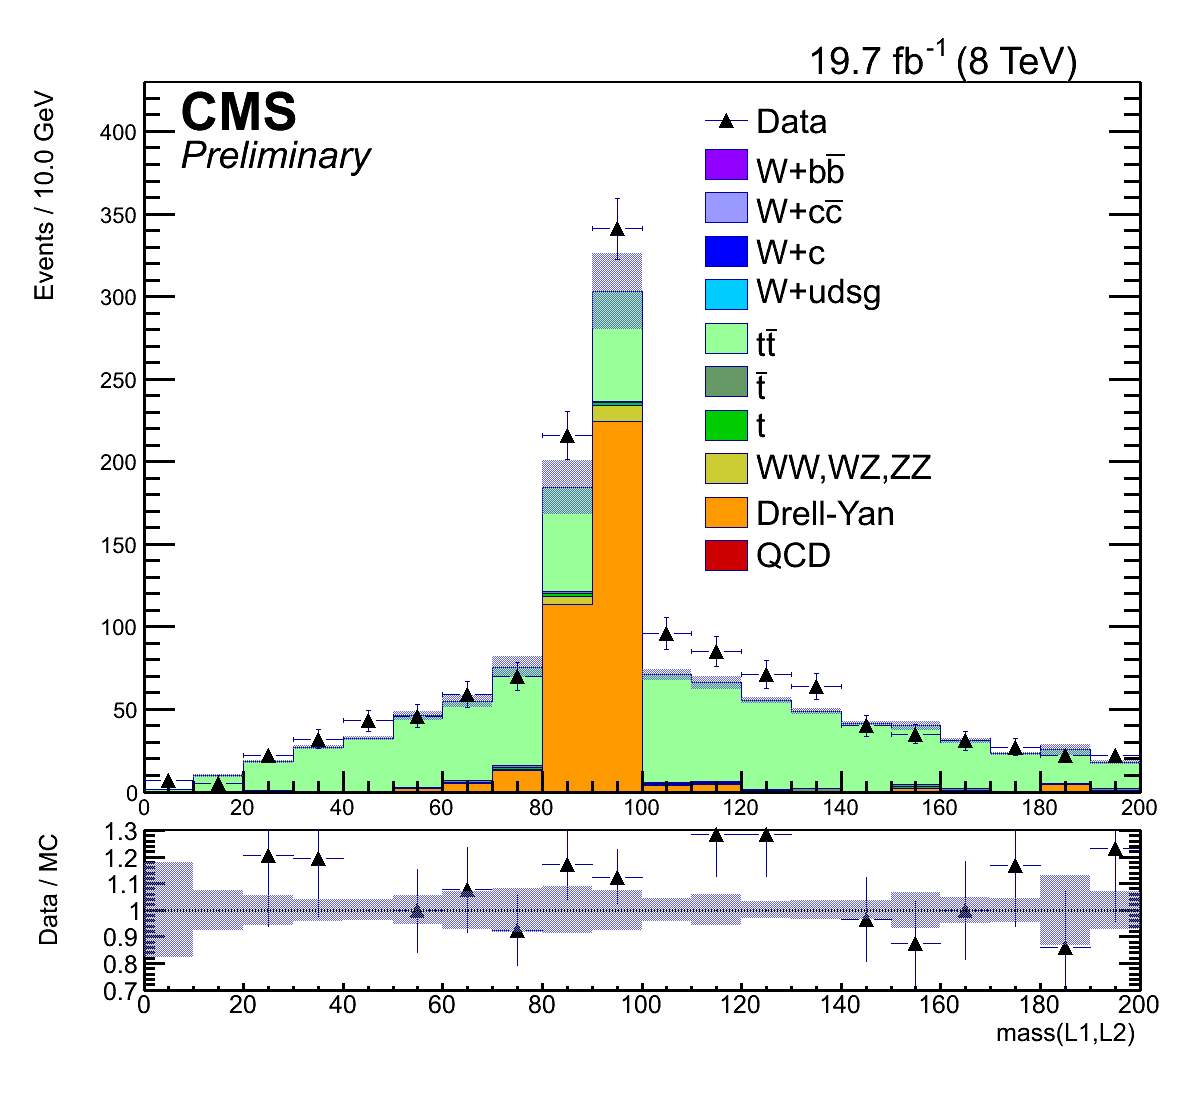
\includegraphics[width=0.4\textwidth]{/Users/rhombus/CMS/Thesis/thesis/pdfs/wbbxc/dy/Histograms_e2CJ_xFJ_tB2_goodL1L2_mass_mu.png}
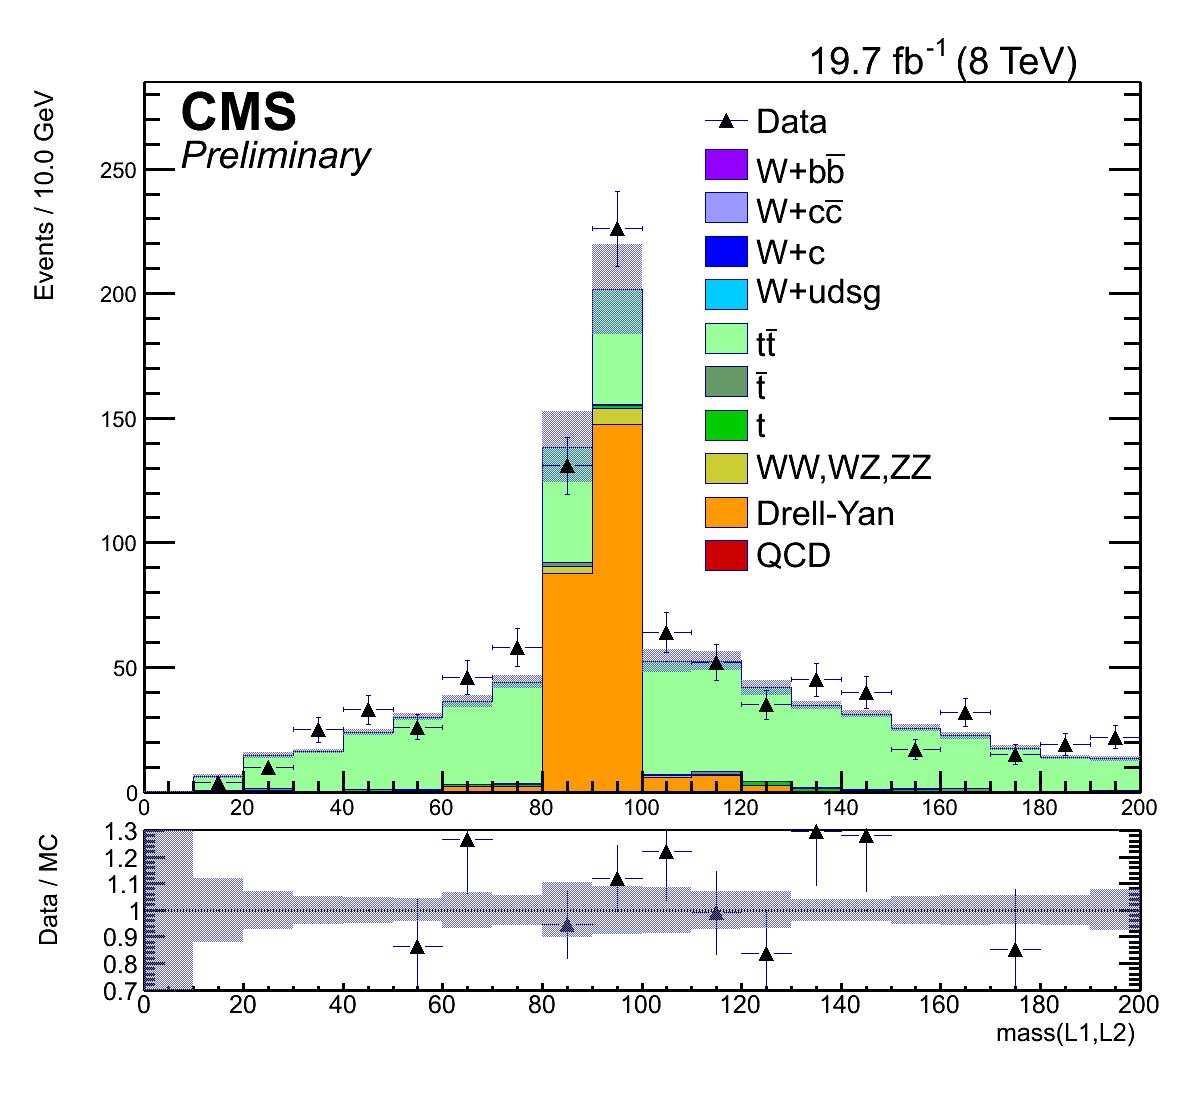
\includegraphics[width=0.4\textwidth]{/Users/rhombus/CMS/Thesis/thesis/pdfs/wbbxc/dy/Histograms_e2CJ_xFJ_tB2_goodL1L2_mass_ele.png}
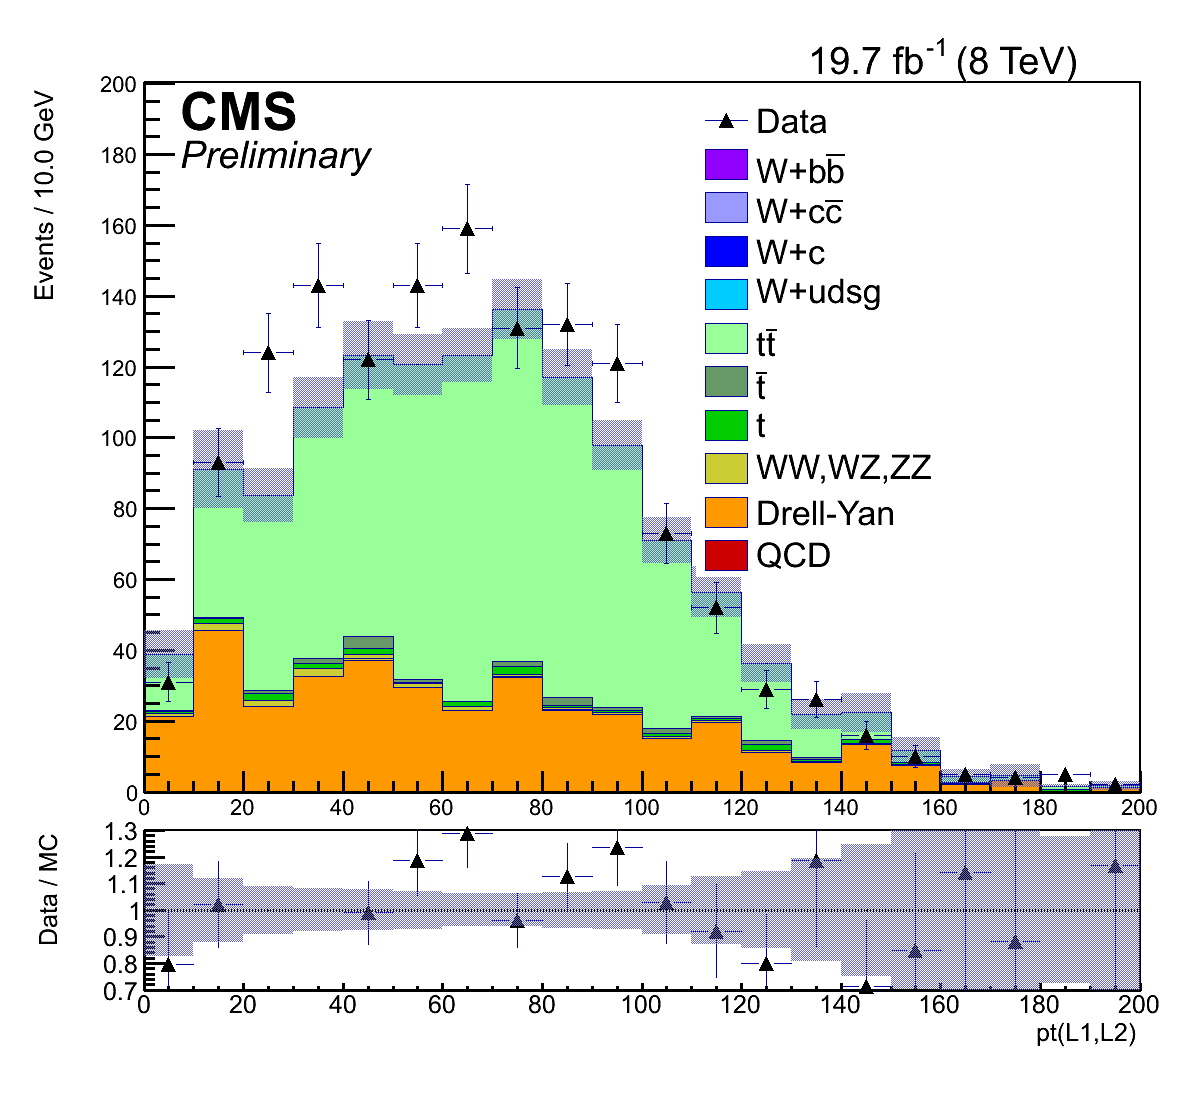
\includegraphics[width=0.4\textwidth]{/Users/rhombus/CMS/Thesis/thesis/pdfs/wbbxc/dy/Histograms_e2CJ_xFJ_tB2_goodL1L2_pt_mu.png}
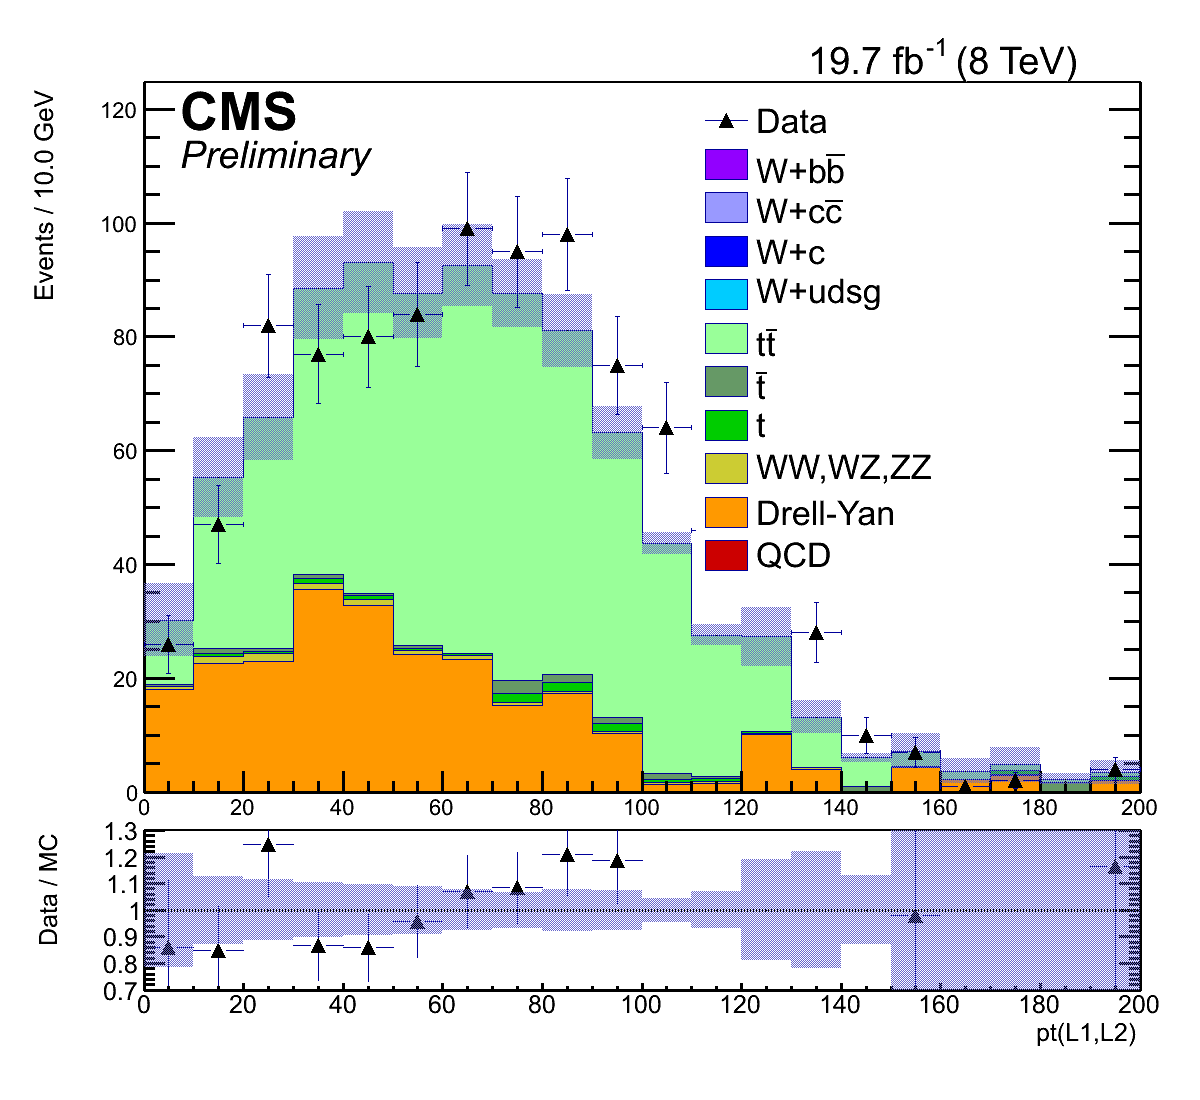
\includegraphics[width=0.4\textwidth]{/Users/rhombus/CMS/Thesis/thesis/pdfs/wbbxc/dy/Histograms_e2CJ_xFJ_tB2_goodL1L2_pt_ele.png}
      \label{fig:prefit_dybb}
\end{figure}

\begin{figure}
      \caption[\zjj control region for the \wbb measurement]{ Above are distributions of the mass and
        transverse momentum of the dilepton pair in the
        $\zjj$ phase space.
       Left plots are in the muon decay channel and right
        plots are in the electron decay channel.
      }
      \center
 \subfloat[]{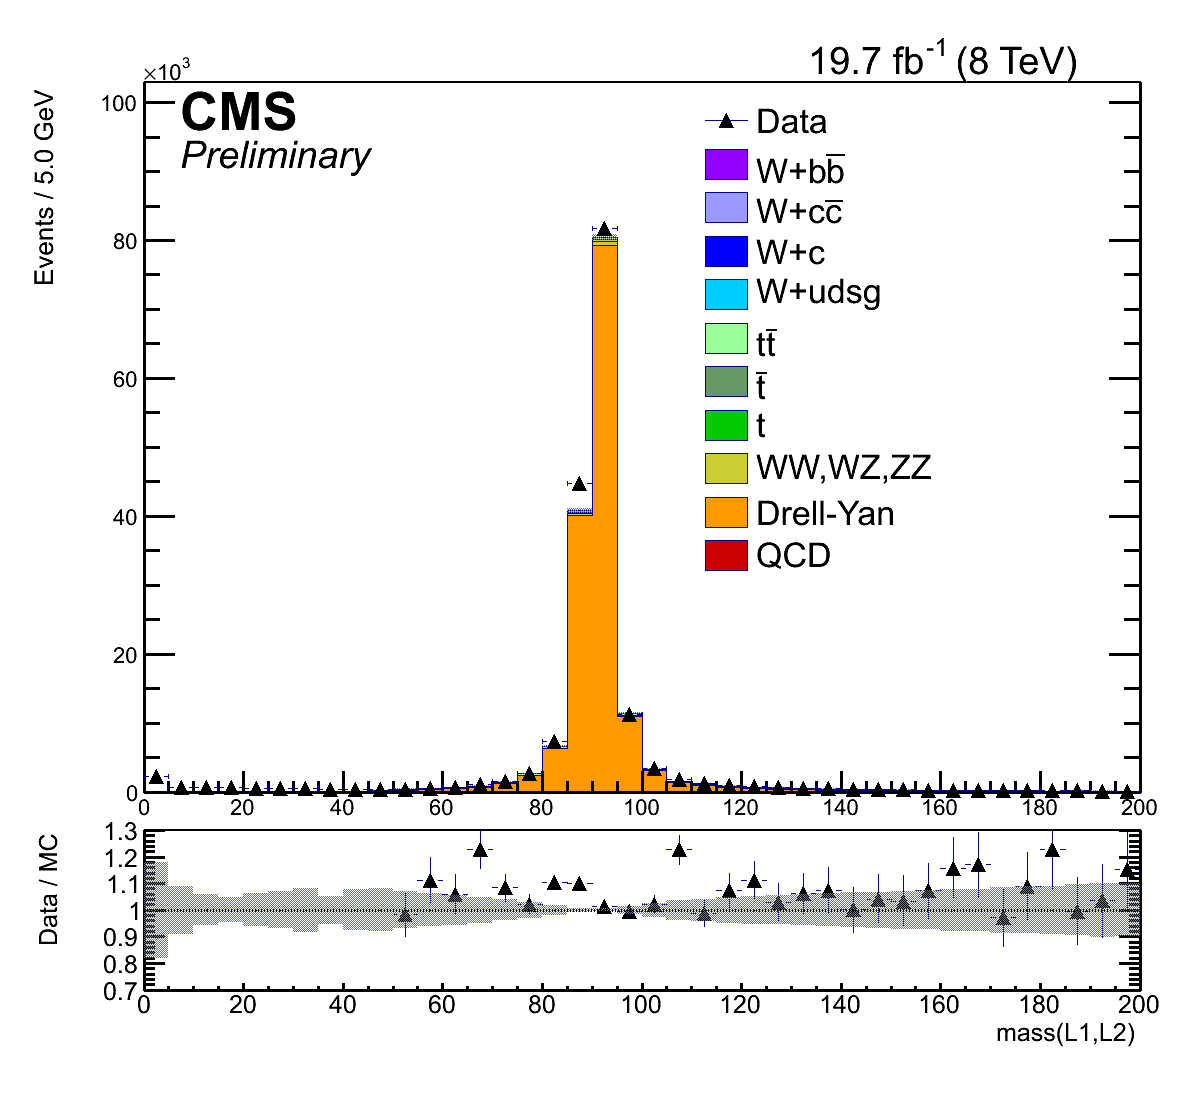
\includegraphics[width=0.4\textwidth]{/Users/rhombus/CMS/Thesis/thesis/pdfs/wbbxc/dy/Histograms_e2CJ_xFJ_goodL1L2_mass_mu.png}}
 \subfloat[]{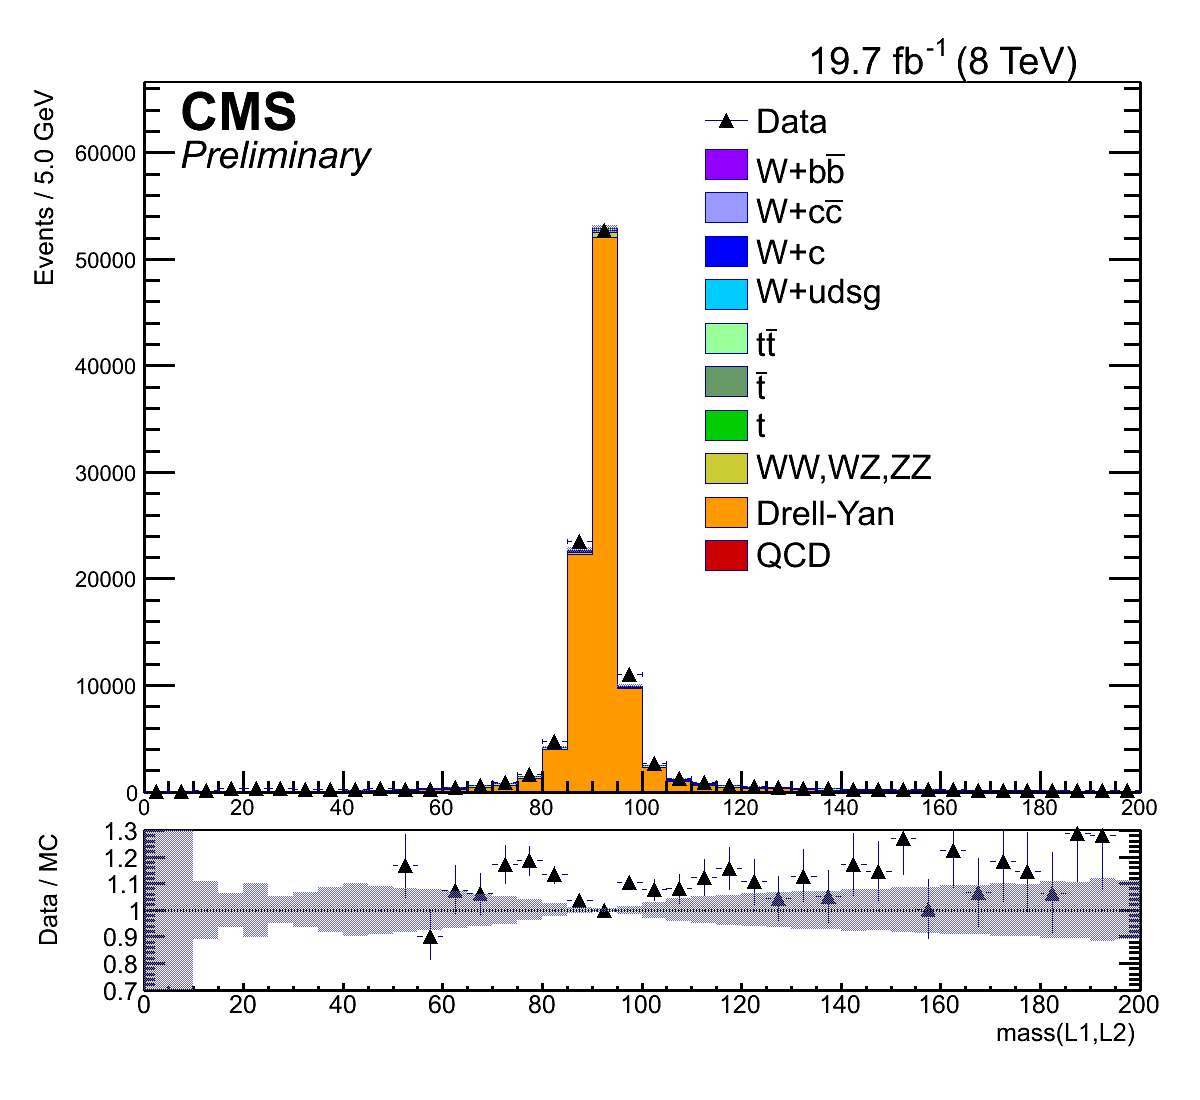
\includegraphics[width=0.4\textwidth]{/Users/rhombus/CMS/Thesis/thesis/pdfs/wbbxc/dy/Histograms_e2CJ_xFJ_goodL1L2_mass_ele.png}}
  \\
 \subfloat[]{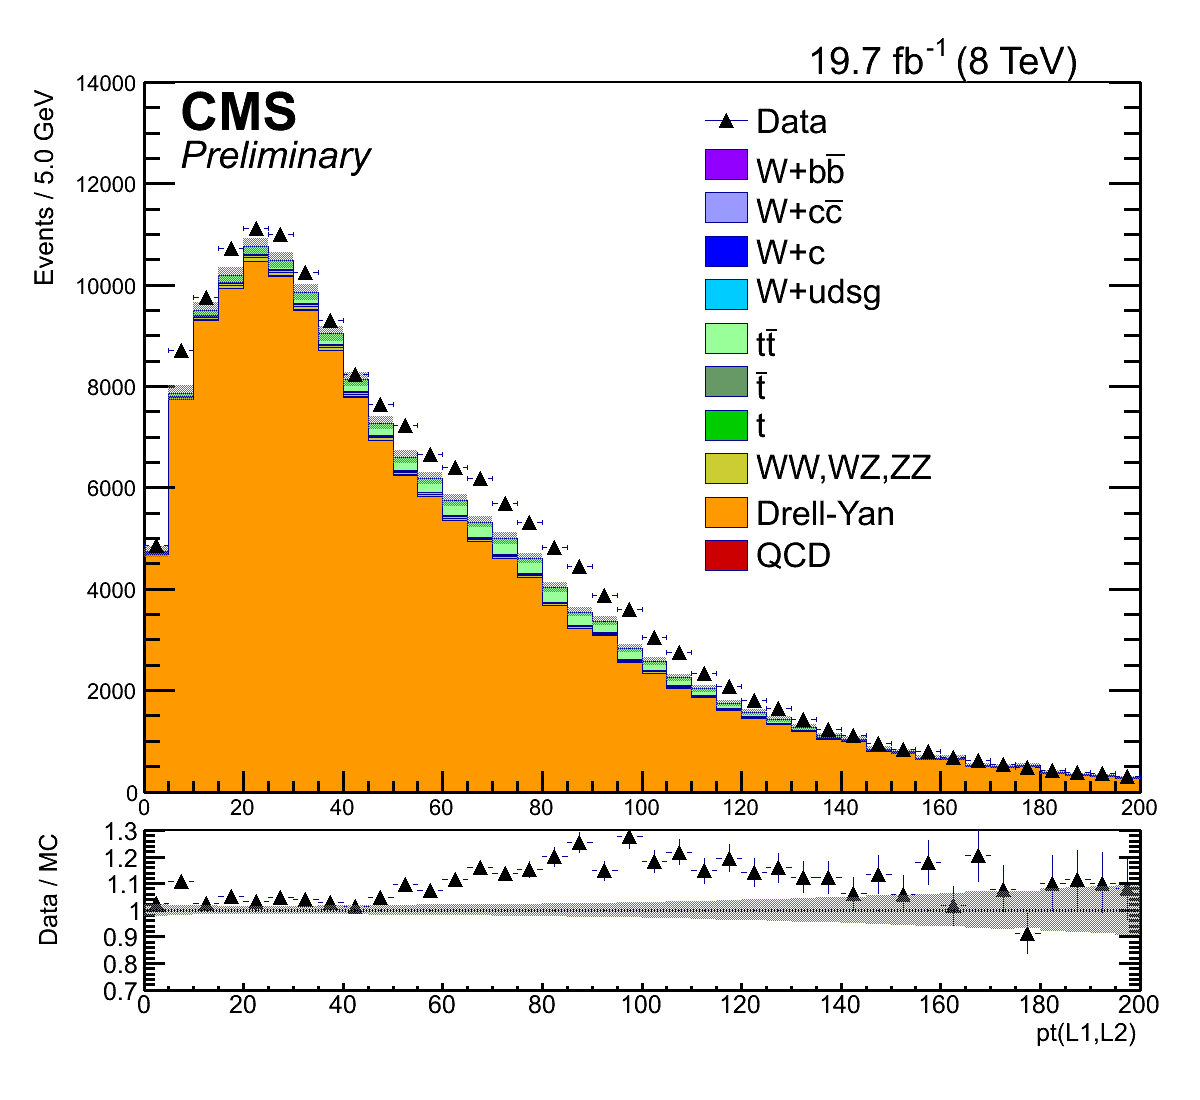
\includegraphics[width=0.4\textwidth]{/Users/rhombus/CMS/Thesis/thesis/pdfs/wbbxc/dy/Histograms_e2CJ_xFJ_goodL1L2_pt_mu.png}}
 \subfloat[]{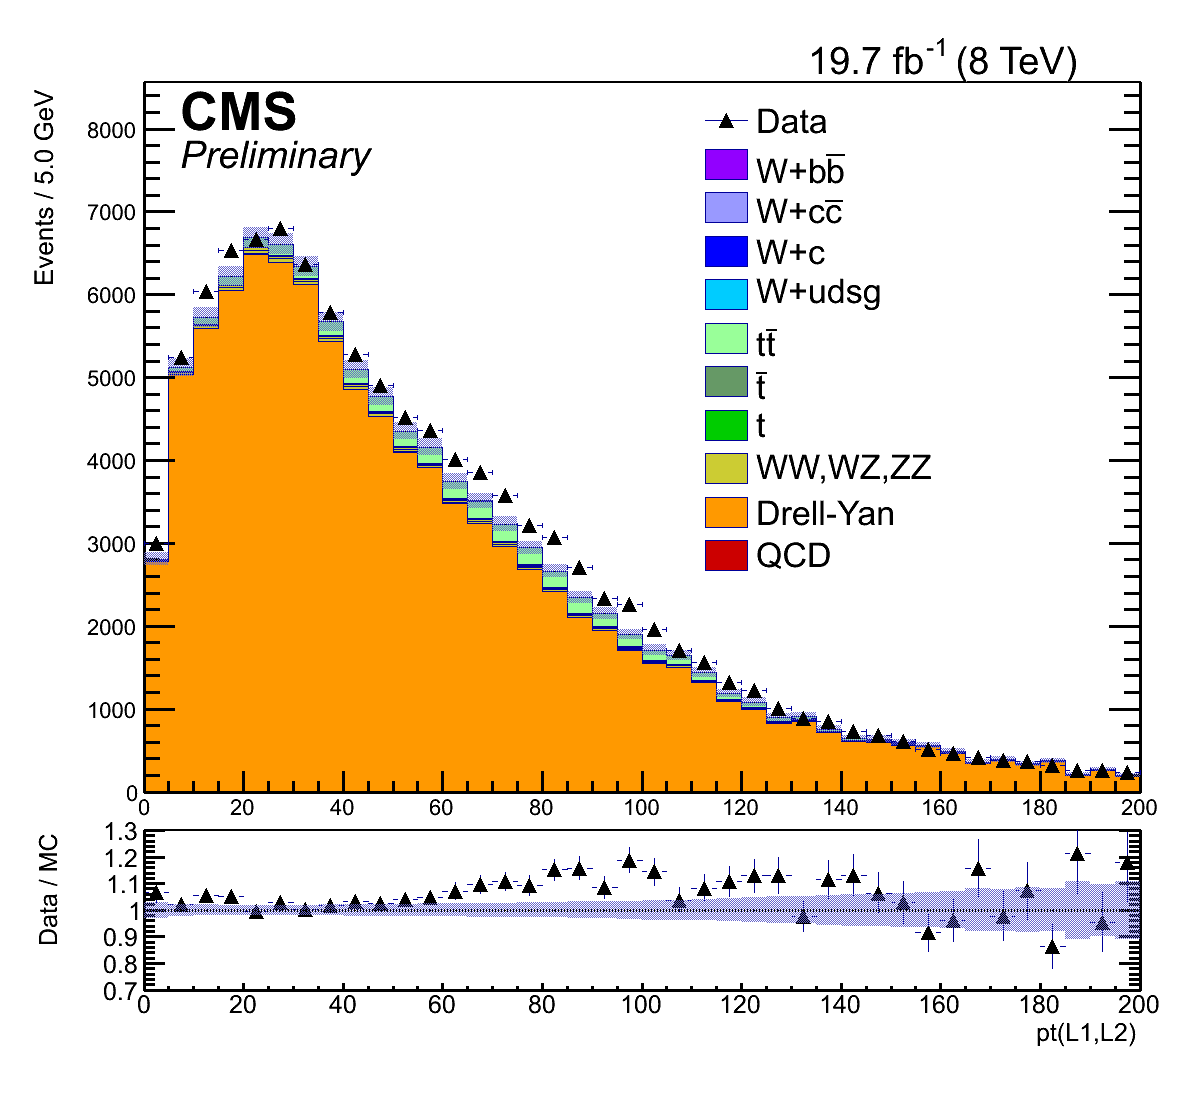
\includegraphics[width=0.4\textwidth]{/Users/rhombus/CMS/Thesis/thesis/pdfs/wbbxc/dy/Histograms_e2CJ_xFJ_goodL1L2_pt_ele.png}}
  \\
      \label{fig:prefit_dyjj}
\end{figure}


\section{Analysis Strategy}\label{subsec:wbb_analysisstrategy}
The $\wbb$ yield is ultimately measured using a likelihood fit
 to the $\mt$ distribution in the signal region,
 after having rescaled the simulation. 
Since the dominant background in the signal region arises
 from the $\ttbar$ process, the data and simulation
 are compared in two $\ttbar$-dominated control regions.
The simulation is reweighted to describe the control regions
 and then is used to predict the $\mt$ distributions
 in the signal region.

%The dominant background in the signal
% region arises from the $\ttbar$ process.
%Data and simulation are hence first compared in two 
% $\ttbar$-dominated control regions and 
% MC scale factors are extracted and 
% applied to the signal region.
%Then a likelihood fit is performed to the $\mt$ 
% distribution in order to extract the $\wbb$ cross section.
%In the fit, interpolations are performed as a log normal for
% uncertainties affecting only the normalization
% of distributions
% and quadratically for uncertainties
% affecting both the shapes and normalizations.

The signal region requires a muon (electron)
 with $\pt > 30$ GeV, pseudorapidity
 $|\eta| < 2.1$, and satisfying $I < 0.12~(0.10)$.
 %as defined in Eq. \ref{eq:iso}.
Exactly two b-tagged jets with
 $\pt > 25$ GeV and
 $|\eta| < 2.4$ are also required. %selected for.
Events with additional leptons with
 $\pt > 10$ GeV and $|\eta| < 2.4$ or
 a third jet with $\pt > 25$ GeV and $|\eta| < 5.0$
 are rejected.
The $\ttbar$-multijet control region is obtained
 using the same selection criteria as in the signal region,
 but requiring at least three jets in the event
 with $\pt>25$ GeV and $|\eta|<2.4$ instead of
 vetoing events which have more than two.
The $\ttbar$-multilepton control region uses
 similar selection criteria as the signal region,
 but changing the lepton requirement from vetoing
 events which contain a second lepton,
 to requiring two isolated leptons of different flavor,
 both with $\pt>30$ GeV and $|\eta|<2.1$.

The shape of the $\wbb$ signal distribution is obtained by separating
 the $\wjets$ simulated sample into three subsamples labeled as $\wbb$, $\wcc$, and $\wudscg$.
The separation is done at the truth generator level.
If an event contains a b jet, from matrix element or parton shower,
 it falls into the $\wbb$ category.
A b jet at generator level requires
 the presence of a b hadron within a cone of
 radius $R=0.4$ with respect to the jet axis.
The jets are constructed at the generated level using
 all stable particles in the event (excluding neutrinos).
Jets with a distance smaller than $R = 0.5$ with respect to a
 lepton are removed from the event.
%Exactly two b jets with $\pt>25\GeV$ and $|\eta|<2.4$
% are required in the signal region.
If an event contains no b jets but
 an even, non-zero, number of charm jets,
 again from matrix element or
 parton shower, it falls into the $\wcc$ category.
The remaining events fall into the $\wudscg$ category.
% hen level definitions
The energy of the selected leptons at the generated level is corrected
 for the final state radiation (FSR) by summing up
 the four-momenta of
 all the photons generated within a cone of radius $R = 0.1$
 around the lepton.
Generated leptons originating in simulation from the decay of b hadrons or $\tau$ leptons
 are not considered.

%The normalizations of the simulated backgrounds are allowed to vary in the fit
% within the uncertainties of the corresponding cross sections
% as listed in Table \ref{tab:input_unc_wbb}.

%The shape of the QCD distribution for each region and lepton
% flavor is estimated from data using samples of events that
% pass all the corresponding region requirements,
% but requiring the muon (electron) to be anti-isolated,
% $I > 0.20~(0.15)$.
%The obtained shapes are corrected for the presence of all other
% backgrounds, estimated from simulation.
%Their contribution is less than 1\% of the QCD rate.
%
%The QCD normalization is adjusted in order to describe
% the number of data events at $\mt<20$ GeV,
% after subtracting the non-QCD backgrounds
% obtained from simulation.
%In the fiducial regions used in this analysis, minimal correlation
% is observed between $I$ and $\mt$, validating
% the use of an inverted isolation requirement to obtain
% the QCD shape.

Two major parameters in the simulations
 significantly affect the shape and
 normalization of the simulated distributions:
 the b-tagging efficiency and the jet energy scale (JES).
Both control and signal regions show similar
 sensitivity to the b-tagging efficiency,
 and its adjustment affects all the regions
 in a correlated manner.
The JES affects more the $\ttbar$ predictions
 in the signal and multilepton regions where a veto
 on the third jet is applied.
The effect on the leading jets is moderate,
 but because of the multijet nature of the $\ttbar$ production,
 the JES variations lead to significant migration of jets
 into and out of the veto region.
The $\ttbar$-multijet control region,
 since it has no veto on the third jet,
 is less sensitive to JES.
The same is observed to be true for the $\wbb$ LO sample
 in all regions and may be due in part to the fact that
 $\wbb$ has no additional jets to veto.

The fit procedure thus consists of three steps.
First, using the simulated samples detailed above,
 a fit is performed in the $\ttbar$-multijet reigion
 using the $\mt$ variable.
The result of this fit gives an estimation of the
 b-tagging effeciency rescaling factor, which
 is measured separately in the muon and electron
 channels and averaged. % before being applied.
The reweighted samples are then used in the next step
 where a fit to the $\mt$ variable in the
 $\ttbar$-multilepton region is performed and
 the jet energy scale in simulation is adjusted.
As a result of these two steps, the simulation is
 expected to properly describe the $\ttbar$ contribution
 and the final step is to extract the number of
 $\wbb$ events from a fit in the signal region.

\section{Systematic Uncertainties}
The major sources of the systematic uncertainties are listed in Table \ref{tab:input_unc_wbb}.
 The size of the variation is presented for each uncertainty source
 together with its effect
 on the signal.
Some of the uncertainties affect
 only the normalization of the respective contributions,
 e.g. the uncertainty on the
 theoretical cross sections.
In other cases, the uncertainties affect also the
 shape of the corresponding $\mt$ distributions,
 and these are listed in
 the table under ``norm. + shape".
In the fit procedure, interpolations are performed following a log
 normal distribution for uncertainties affecting only normalizations
 and a quadratic distribution for uncertainties affecting both the shapes and normalizations.

The 50\% uncertainty on the QCD background is taken as a conservative estimate from
 the control region, and increasing this uncertainty does not lead to any change
 in the result of the fit.
The common b-tagging and JES rescaling factor uncertainties
 are set to $\pm100\%$ of the factor itself, allowing the fit to
 remeasure them in the signal region.
The scale uncertainties are estimated by
 changing the renormalization and factorization scales
 up and down by a factor of two.
The PDF uncertainties are estimated from the change in
 acceptance found by varying the
 PDF set.

\begin{table}[htb]
\begin{center}
\caption[Systematic uncertainties in $\wbb$]{
Breakdown of the major sources of systematic
 uncertainty in the \wbb phase space.
The last column indicates the contribution of
 the given systematic to the overall uncertainty
 on the measured cross section. %signal strength.
The uncertainty labeled "b tag rescale" is
 the uncertainty associated with the rescaling
 of the b tag efficiency scale factors.
In the "variation" column, the uncertainties which
 are correlated across all simulated samples and
 affect both shape and normalization are indicated
 by $\sigma_{\mathrm{X}}$ to indicate that an input variation of
 one standard deviation is set on the uncertainty X in the fitting procedure.
UES refers to the energy scale of energy deposits
 not clustered into jets and MES and EES
 refer to the muon and electron energy scales.
The uncertainty labeled as "Id/Iso/Trg" is the uncertainty
 associated with the efficiency of the lepton
 identification, isolation, and triggering.
The uncertainty on the luminosity and the uncertainty
 on the acceptance due to PDF and scale choices are
 not included in the fit, and are
 treated separately.
}
\label{tab:input_unc_wbb}

%\resizebox{\columnwidth}{!}{%
{\renewcommand{\arraystretch}{1.2}
\begin{tabular}{c|c|l|l|l}
\multicolumn{2}{c|}{}                                                         & {}            & {}        & effect on the measured \\
{} & {}                                                                       & uncertainty   & variation & cross section \\
\hline
\hline
 \multirow{11}{*}{\rotatebox{90}{normalization}} & \multirow{8}{*}{\rotatebox{90}{uncorrelated}} & \ttbar        & 7.4\%     & 10.5\%  \\
            {}                                   &           {}                                  & Single Top    & 5.4\%     & 3.3\%  \\
            {}                                   &           {}                                  &    \wudscg    & 13.2\%    & $<2\%$  \\
            {}                                   &           {}                                  &       \wcc    & 8.1\%     & $<2\%$ \\
            {}                                   &           {}                                  &    Diboson    & 8.1\%     & $<2\%$  \\
            {}                                   &           {}                                  &  Drell-Yan    & 7.9\%     & $<2\%$ \\
            {}                                   &           {}                                  & $\gamma$+jets & 10.0\%    & $<2\%$ \\
            {}                                   &           {}                                  &        QCD    & 50\%      & 1-4\% \\
\cline{2-5}
\noalign{\smallskip}
\cline{2-5}
            {}                                   &\multirow{9}{*}{\rotatebox{90}{correlated}}    & b tag rescale & 12.9\%              & 13.0\% \\
            {}                                   &           {}                                  & JES rescale   & $1.3\times\sigma_{\mathrm{JES}}$ & $3.6\%$ \\
\cline{1-1} \cline{3-5}
 \multirow{5}{*}{\rotatebox{90}{norm. + shape}}  &           {}                                  & JES           & $\sigma_{\mathrm{JES}}$ & 5.6\%  \\
            {}                                   &           {}                                  & UES           & $\sigma_{\mathrm{UES}}$ & 2.8\% \\
            {}                                   &           {}                                  & MES           & $\sigma_{\mathrm{MES}}$ & 3.6\% \\
            {}                                   &           {}                                  & EES           & $\sigma_{\mathrm{EES}}$ & $<2\%$ \\ %$3.5\% \\ 
            {}                                   &           {}                                  & Id/Iso/Trg    & $\sigma_{\mathrm{Id/Iso/Trg}}$ & $<2\%$ \\
\hline
\hline
            \multicolumn{3}{c|}{luminosity}         & \multicolumn{2}{c}{2.6\%}  \\
            \multicolumn{3}{c|}{theory (scale+PDF)} & \multicolumn{2}{c}{10\%}   \\


\end{tabular}
}
%\end{adjustwidth}
\end{center}
\end{table}

\section{Signal Extraction}

\label{sec:results}

The fit in the $\ttbar$-multijet region
 is used to obtain rescaling factors for
 the muon and electron channels separately
 to better describe the
 b-tagging efficiency in the simulation,
 as presented in Section \ref{subsec:wbb_analysisstrategy}.
The results of the fit are presented in Fig. \ref{fig:step1_ttjjj_fitted}.
The measured rescaling factors, $1.17 \pm 0.12$ (muon channel) and
 $1.13 \pm 0.11$ (electron channel), are averaged to $1.15 \pm 0.14$, where
 the uncertainty allows the following fits to
 vary the rescaling factor between 1.01 and 1.29.
 %and with the bounds given by the fits in the individual channels.
The simulation is rescaled accordingly for the next fit and
 the uncertainty on the rescaling is included in the fit procedure.

\begin{figure}[htbp]
\caption[$\ttbar$-multijet control region after fitting for b-tag scale]
 {
  The transverse mass distributions in the $\ttbar$-multijet phase space after fitting to obtain the b-tag rescale factors.
  The lepton channels are shown separately with the muon sample on the left and the electron sample on the right.
  The highest bin contains overflow events.
 The shaded area represents the total uncertainty on the simulation as output from the fit.
 }
\center
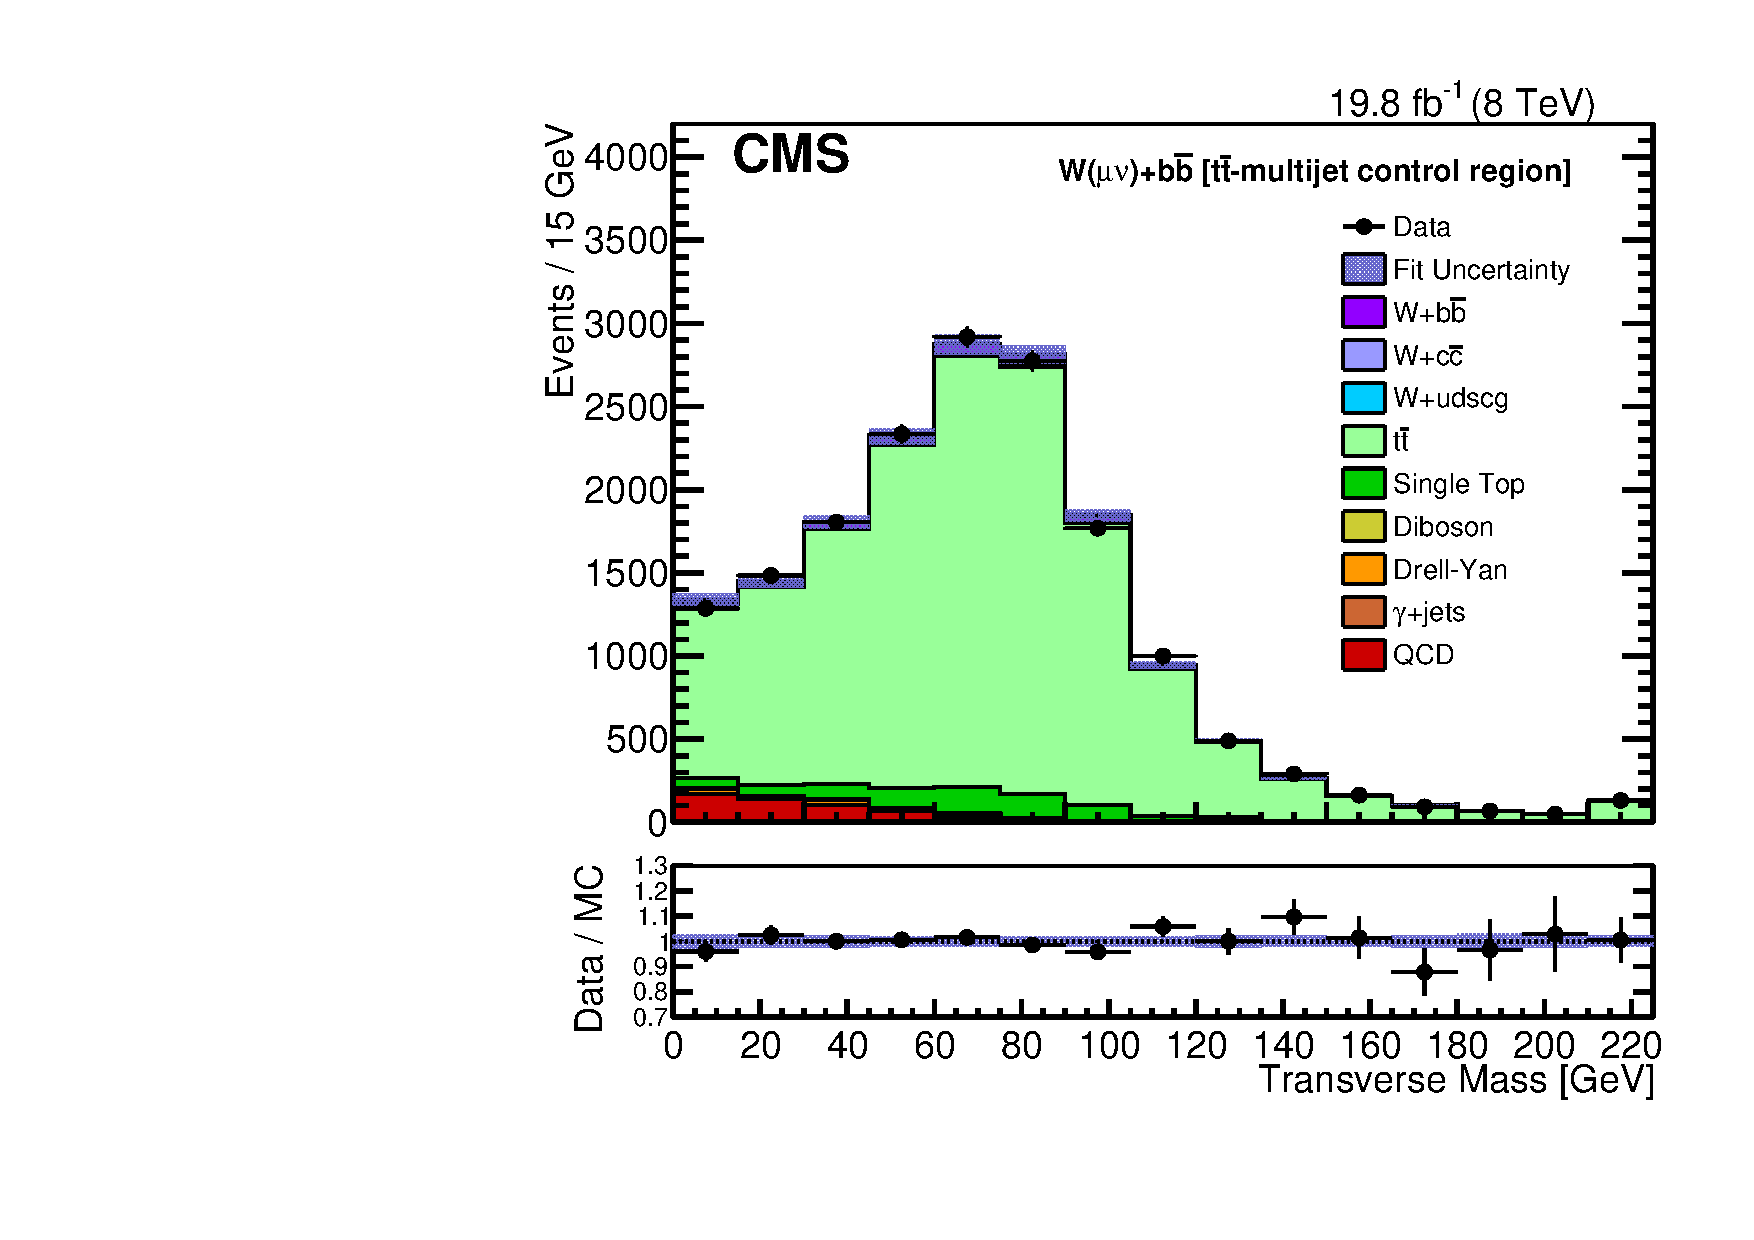
\includegraphics[width=0.49\textwidth]{/Users/rhombus/CMS/Thesis/thesis/pdfs/wbbxc/pape/poststep1_ttjjj_mt_mu}
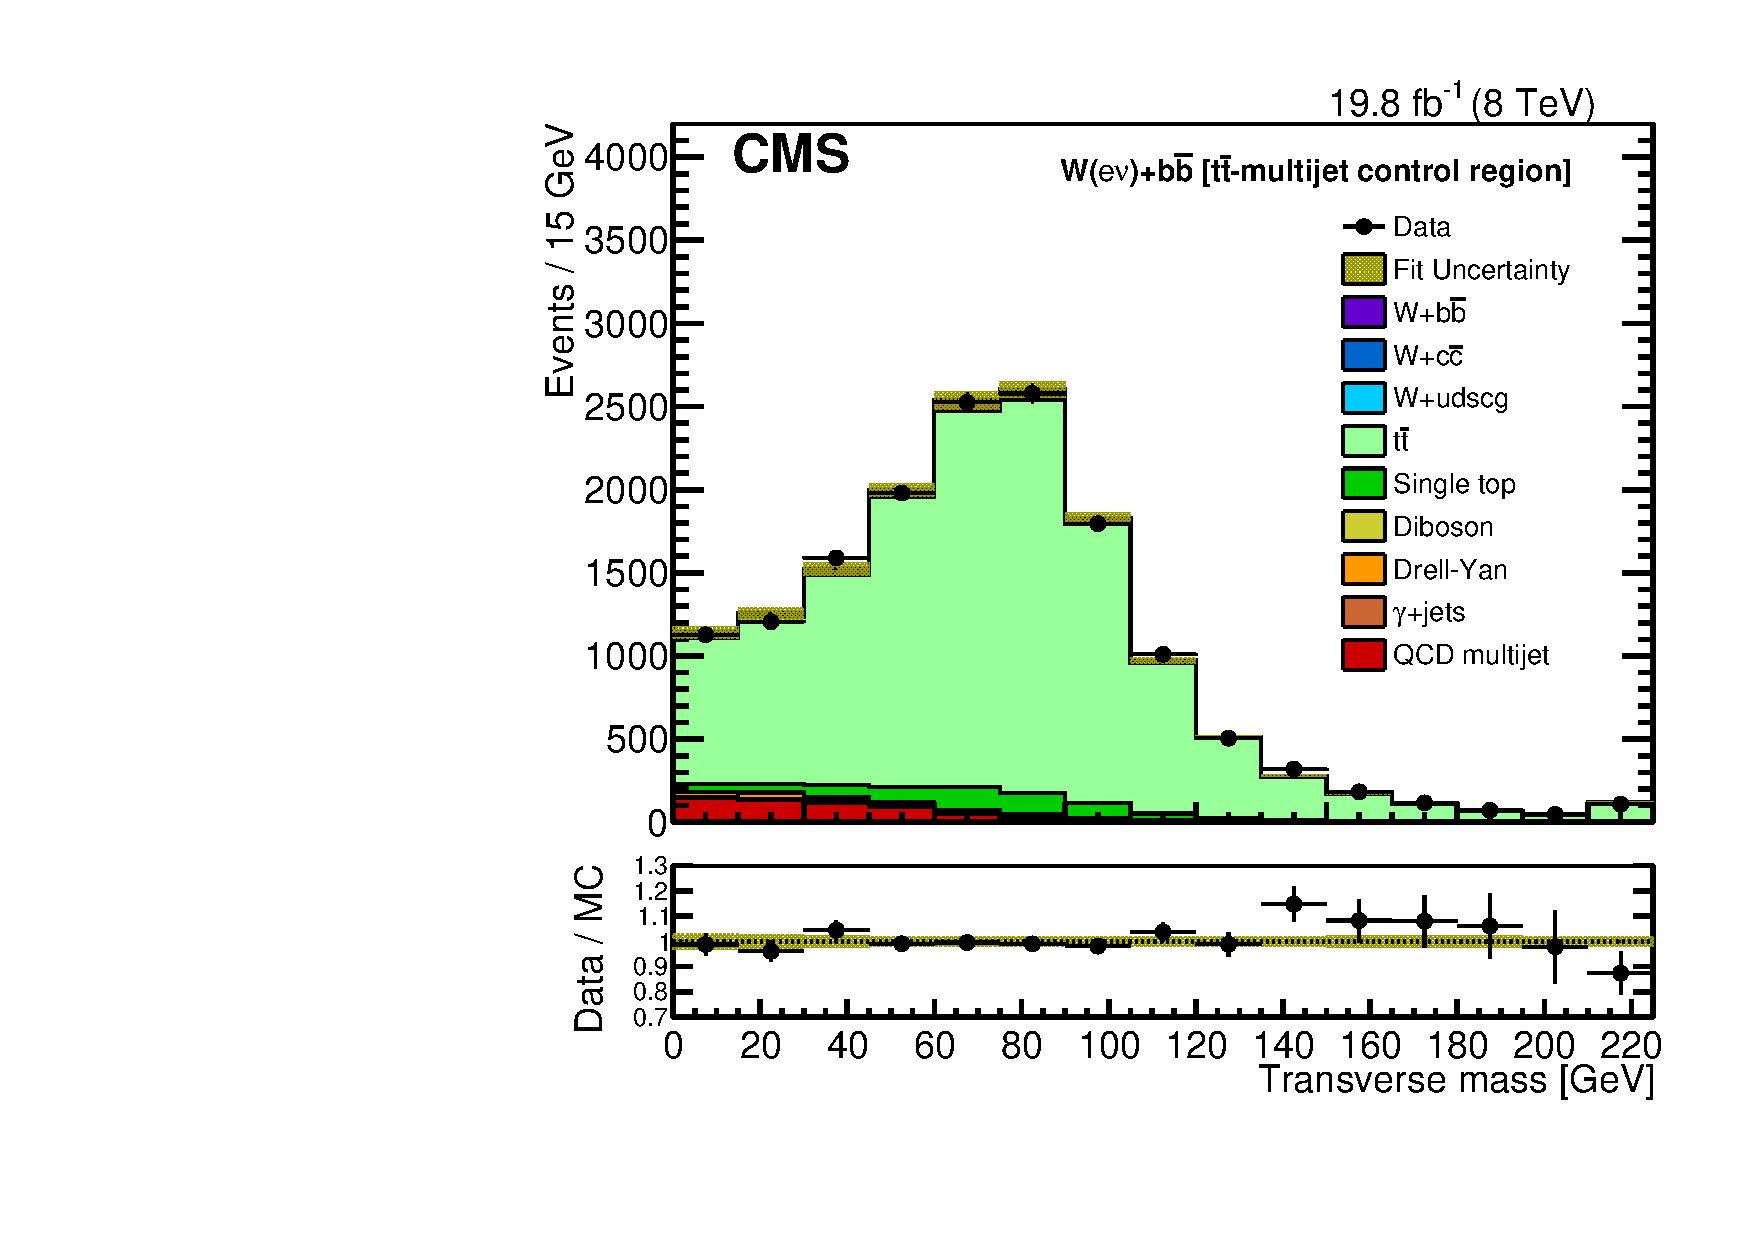
\includegraphics[width=0.49\textwidth]{/Users/rhombus/CMS/Thesis/thesis/pdfs/wbbxc/pape/poststep1_ttjjj_mt_ele}
\label{fig:step1_ttjjj_fitted}
\end{figure}

A fit to the $\ttbar$-multilepton region adjusts
 the jet energy scale, as described in Section \ref{subsec:wbb_analysisstrategy}.
%The energy scale in the fit varies within its uncertainties, $\sigma_{\mathrm{JES}}$.
As a result, the simulated $\mt$ distributions
 change both the shape and normalization.
The best fit suggests changing the
 JES by approximately 1.3$\sigma_{\mathrm{JES}}$ from its central value.
Figure \ref{fig:step2_ttme_fitted}
 shows the results of the fits in the $\ttbar$-multilepton
 enhanced data set for
 the muon channel (left)
 and the electron channel (right).
The JES is therefore shifted by 1.3$\sigma_{\mathrm{JES}}$ in
 the simulation with the uncertainty
 set to 1.3$\sigma_{\mathrm{JES}}$.
Thus the simulation is tuned to describe the $\ttbar$
 control regions and is
 used to extract the signal yield in the signal region.

\begin{figure}[htbp]
\caption[$\ttbar$-multilepton control region after fitting for JES]{
  The transverse mass distributions in the $\ttbar$-multilepton enhanced data set after
   fitting to find the appropriate jet energy scale.
  The lepton channels are shown separately with the muon sample on the left and the electron sample on the right.
  The highest bin contains overflow events.
 The shaded area represents the total uncertainty on the simulation as output from the fit.
 }
\center
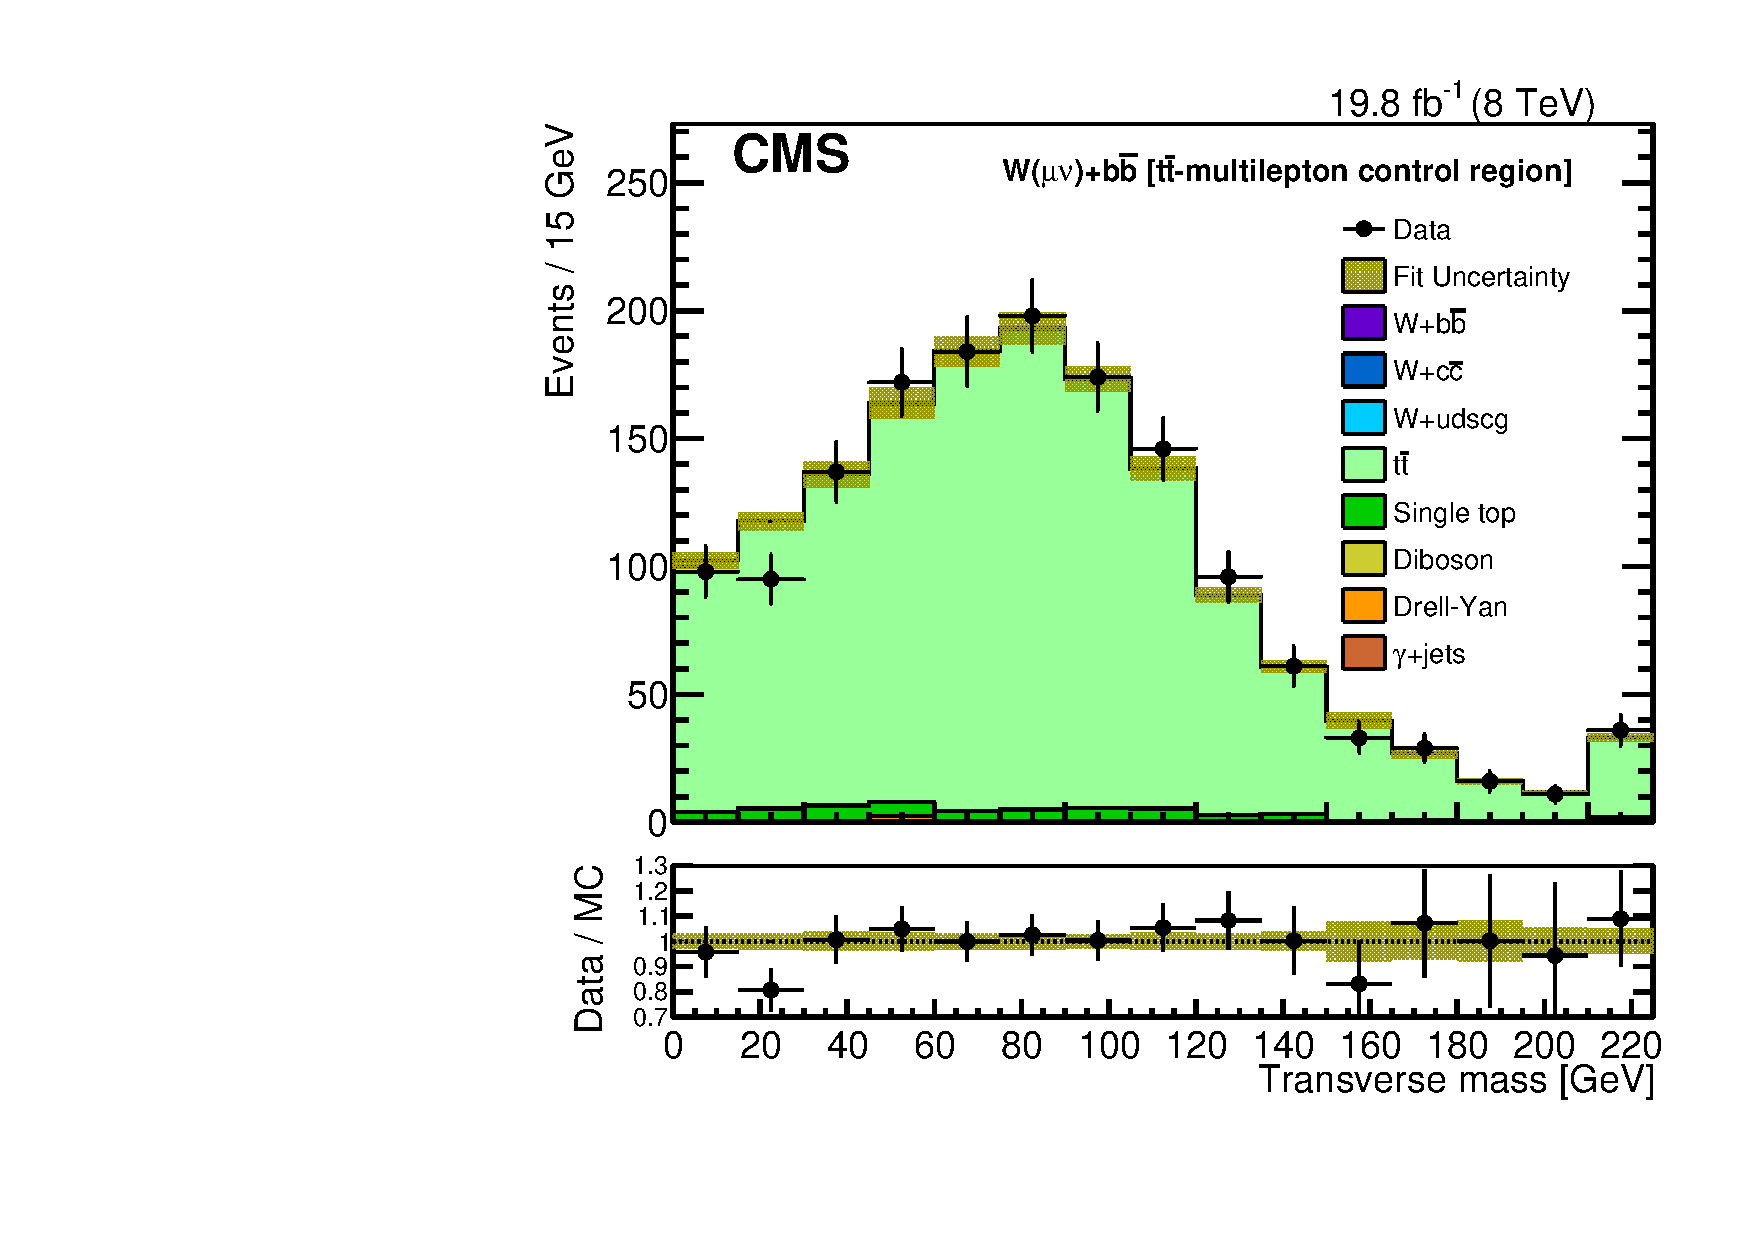
\includegraphics[width=0.49\textwidth]{/Users/rhombus/CMS/Thesis/thesis/pdfs/wbbxc/pape/poststep2_ttme_mt_mu}
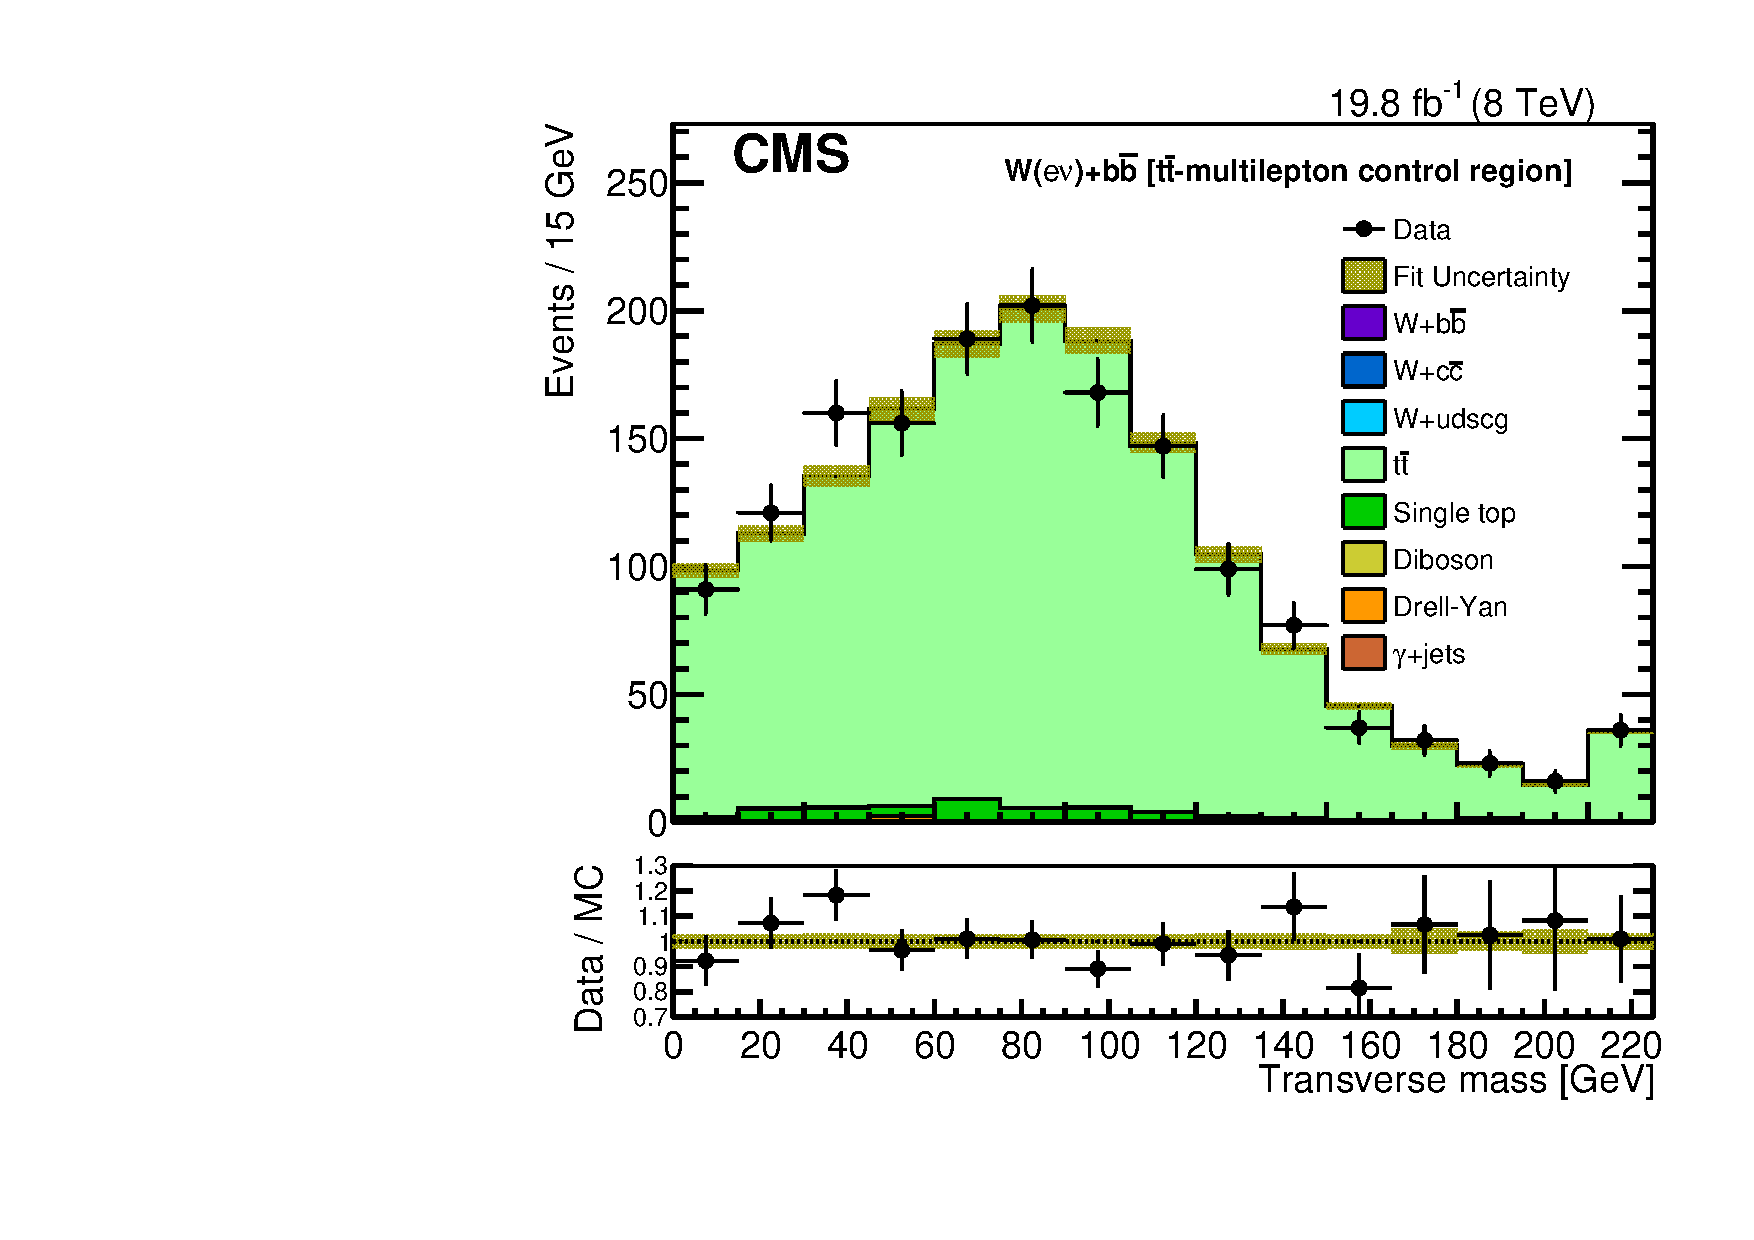
\includegraphics[width=0.49\textwidth]{/Users/rhombus/CMS/Thesis/thesis/pdfs/wbbxc/pape/poststep2_ttme_mt_ele}
\label{fig:step2_ttme_fitted}
\end{figure}

The results of the fit in the $\wbb$ signal region
 are presented in Fig. \ref{fig:step3b_wbb_fitted}.
All background contributions are allowed to vary
 in the fit within their uncertainties,
 while the $\wbb$ normalization remains a free parameter of the fit.
The correlation between different sources of uncertainties
 is taken into account.
The composition of the event sample in
 the signal region is summarized in Table \ref{tab:wbb_yields}.
Events coming from the production of a Higgs boson in association
 with a vector boson constitute a negligible fraction of the
 overall event yield.

Distributions for variables other than those being directly fitted are
 also produced by applying the results from the three fits to
 the simulated samples.
In the signal phase space, lepton isolation was found to be essentially uncorrelated
 with the shape of the transverse mass variable for QCD events,
 but this was not the case for the $\Delta R$ distance between the
 two b-tagged jets, $\Delta R(\mathrm{\bbbar})$, or the lepton $\pt$.
The shape of the QCD distribution for these variables was therefore
 taken from an $\mt<30$ GeV sideband (as opposed to the inverted isolation
 sideband used for the $\mt$ variable) and the normalization
 set to the final fitted normalization given in Table \ref{tab:wbb_yields}.
Distributions of $\Delta R(\mathrm{\bbbar})$ and $\pt^\ell$ in the
 combined lepton channel are presented in Fig. \ref{fig:postfit_drbb_ptl}.
Agreement between data and simulation is observed.

% mt postfit combined lepton fit
\begin{figure}[!htb]
\caption[Fitted \mt in the \wbb signal region]{
  Transverse mass distributions in the $\wbb$ signal region after
   fitting simultaneously muon and electron decay channels.
  The lepton channels are shown separately with the muon sample on the left and the electron sample on the right.
  The highest bin contains overflow events.
  The shaded area represents the total uncertainty on the simulation as output from the fit.
 }
\center
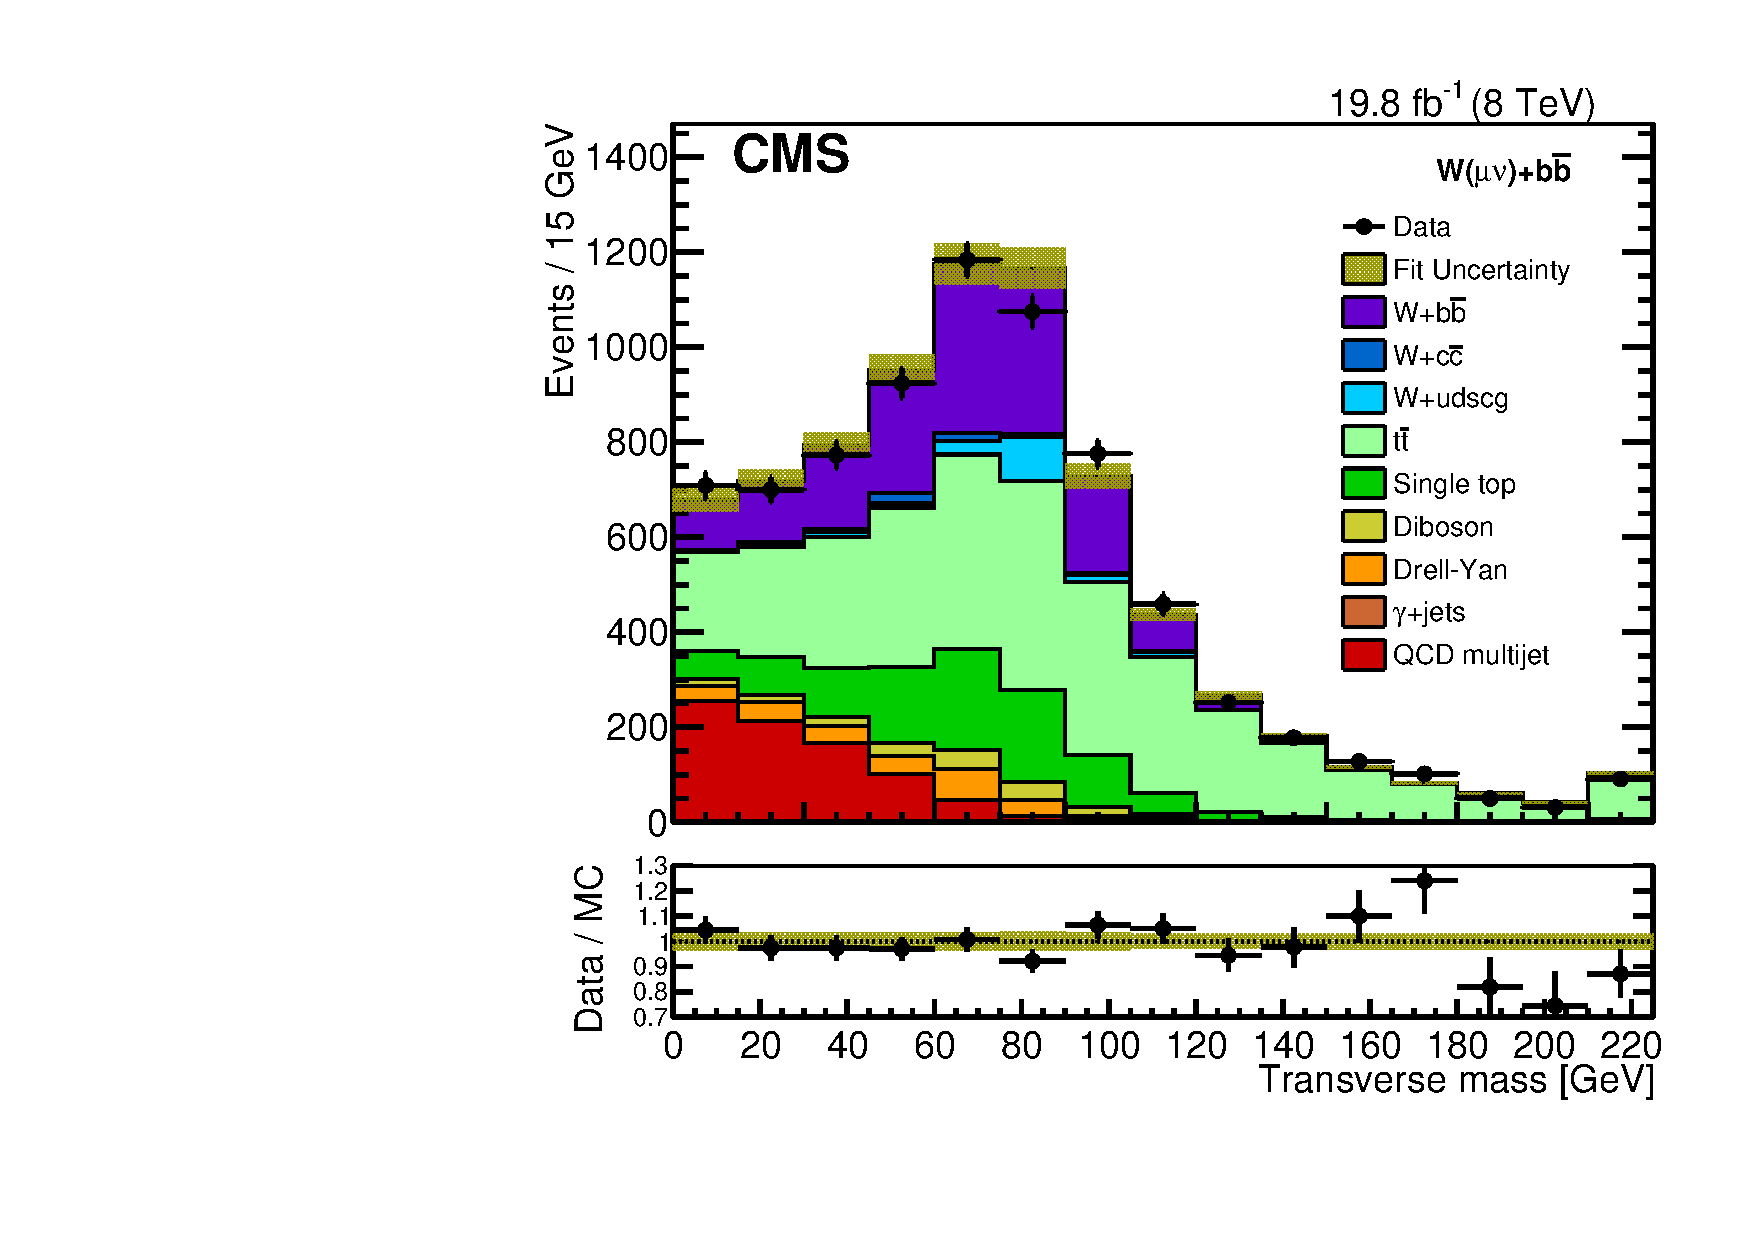
\includegraphics[width=0.49\textwidth]{/Users/rhombus/CMS/Thesis/thesis/pdfs/wbbxc/pape/postcfit_wbb_mt_mu}
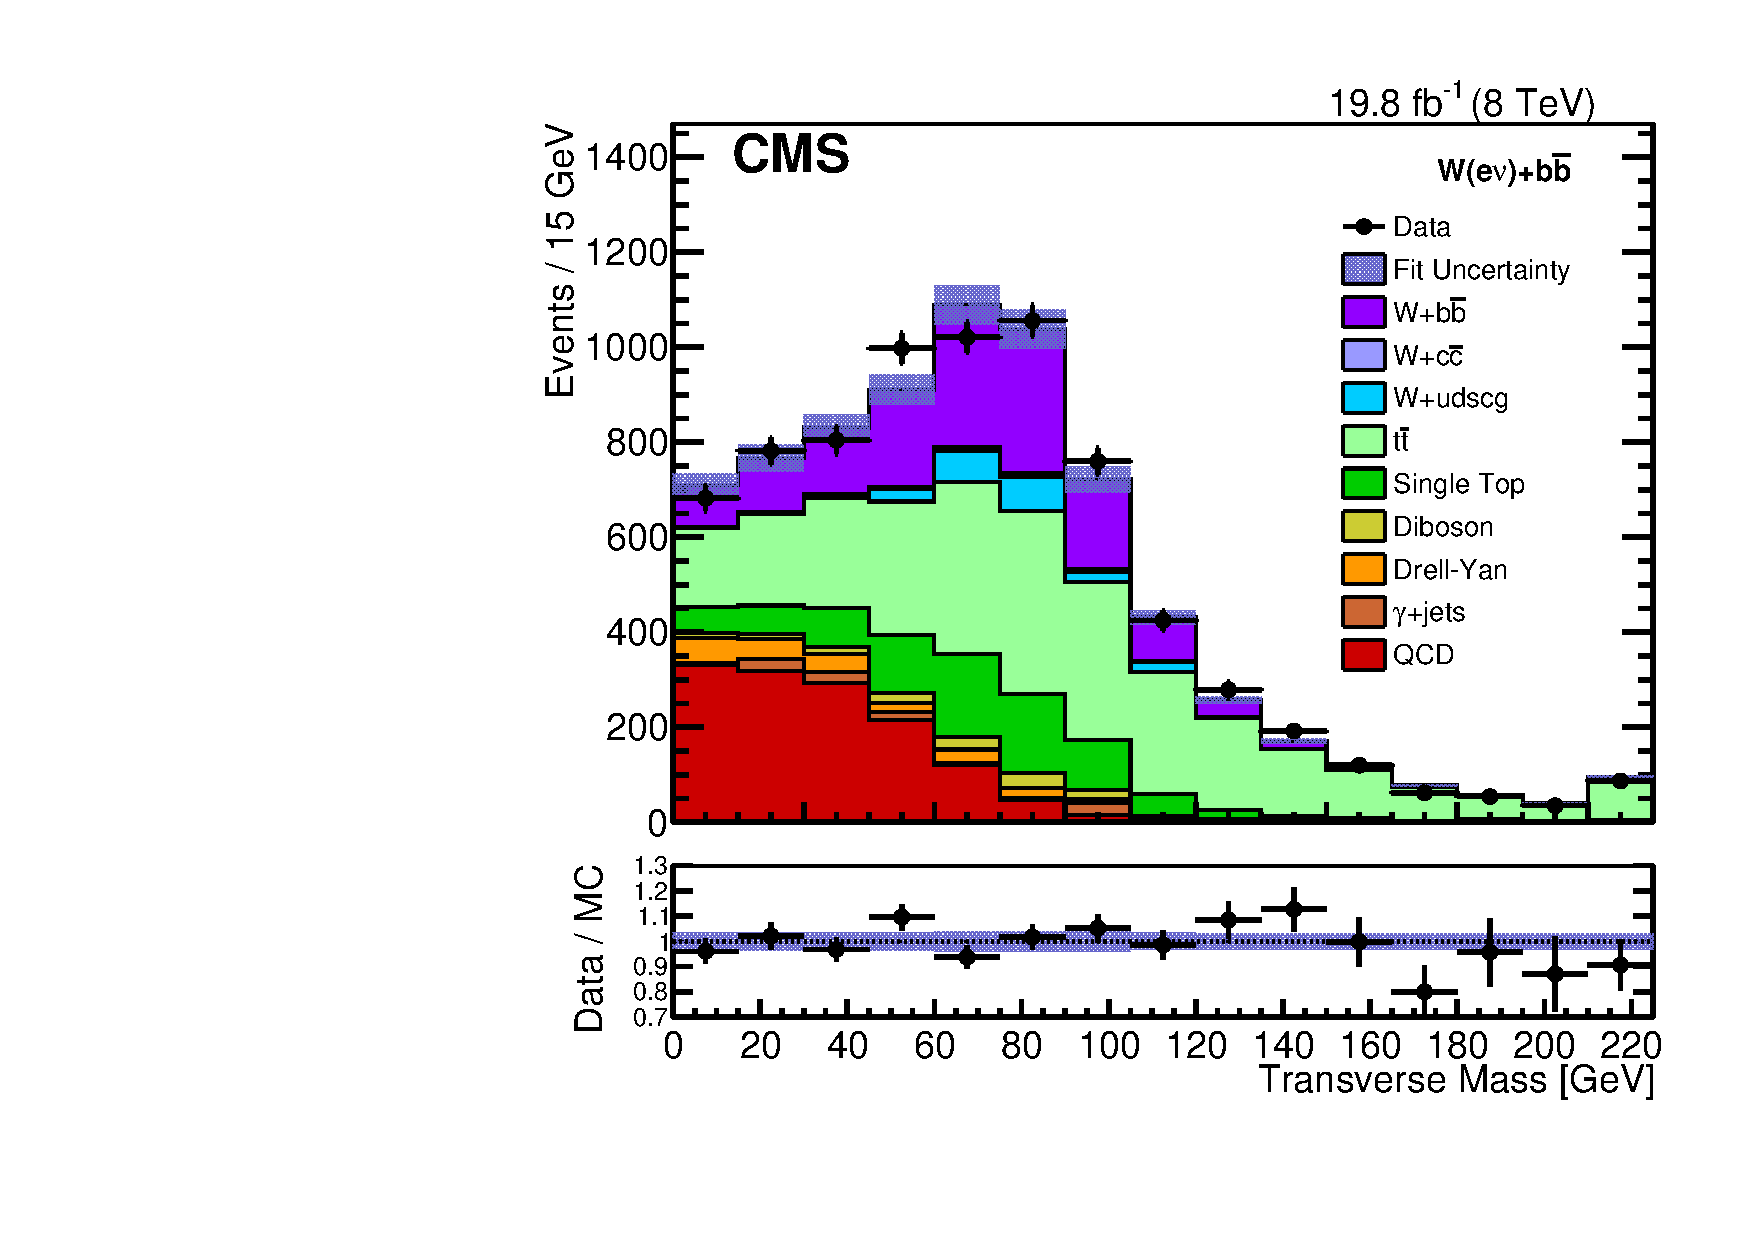
\includegraphics[width=0.49\textwidth]{/Users/rhombus/CMS/Thesis/thesis/pdfs/wbbxc/pape/postcfit_wbb_mt_ele}
\label{fig:step3b_wbb_fitted}
\end{figure}

% Final Fitted Yields
\begin{table}[!htb]
\begin{center}
\caption[Initial and final yields in the $\wbb$ signal region]{
 Initial and final yields obtained in the $\wbb$ signal region.
 The uncertainties on the signal strength represent the
  total uncertainty of the measurement.
}
\label{tab:wbb_yields}
 \begin{tabular}{r|l|l|l|l}
{}       & \multicolumn{2}{c|}{muon}   & \multicolumn{2}{c}{electron}   \\
{}       & Initial      & Fitted      & Initial       & Fitted       \\
\hline \hline
Data     & \multicolumn{2}{c|}{7432}   & \multicolumn{2}{c}{7357}     \\
\hline
\wbb           & 1322.7 & 1731.0 & 1120.5 & 1495.3  \\
\wcc           &   59.7 &   57.4 &   36.0 &   37.2  \\
\wudscg        &  181.7 &  173.8 &  220.0 &  214.3  \\
\ttbar         & 3048.6 & 3276.8 & 2639.6 & 2891.7  \\
Single Top     &  958.0 &  980.1 &  820.2 &  855.5  \\
Drell-Yan      &  261.2 &  262.3 &  220.4 &  225.1  \\
Diboson        &  175.4 &  178.9 &  138.9 &  144.4  \\
$\gamma+$jets  &    0.0 &    0.0 &   98.3 &  104.7  \\
QCD            & 1109.0 &  816.9 & 1653.8 & 1348.0  \\
\hline
\hline
Signal strength & \multicolumn{2}{c|}{$1.21\pm0.24$} &  \multicolumn{2}{c}{$1.35\pm0.28$} \\
\hline
Combined        & \multicolumn{4}{c}{$1.29\pm0.22$} \\
 \end{tabular}
\end{center}
\end{table}

% dR(jj) and pT(l) postfit 
\begin{figure}[!htb]
\caption[Fitted $\Delta R(b\overline{b})$ and $\pt^\ell$ in the \wbb signal region]{
  Distributions of $\Delta R(\mathrm{b\bar{b}})$ and $\pt^\ell$ after
   applying the results from the fits to the simulation.
  The QCD shape was taken from an $\mt<30$ GeV sideband and the
   electron and muon channels have been combined in these distributions.
  The highest bin contains overflow events and
   the shaded area represents the total uncertainty on the simulation as output from the fit.
 }
\center
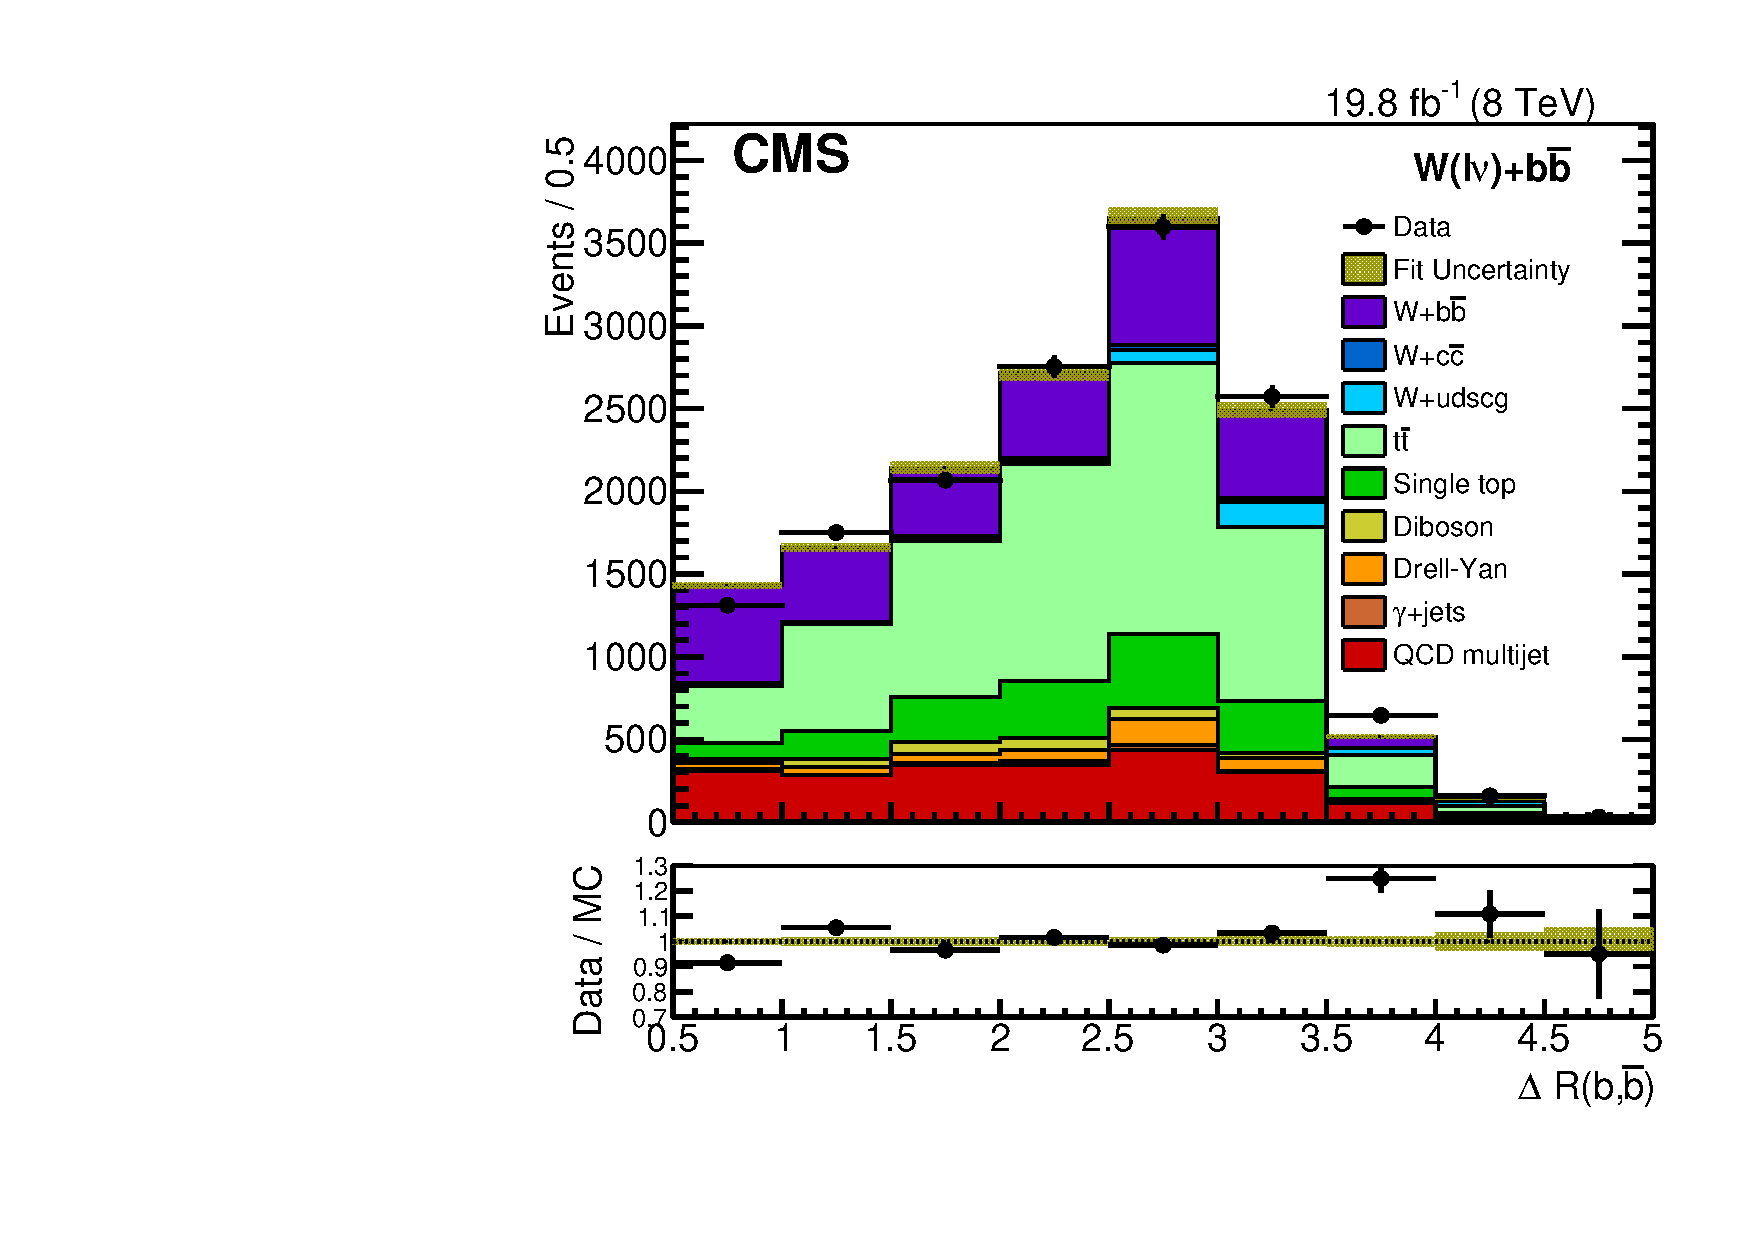
\includegraphics[width=0.49\textwidth]{/Users/rhombus/CMS/Thesis/thesis/pdfs/wbbxc/pape/postcfit_wbb_dRJ1J2}
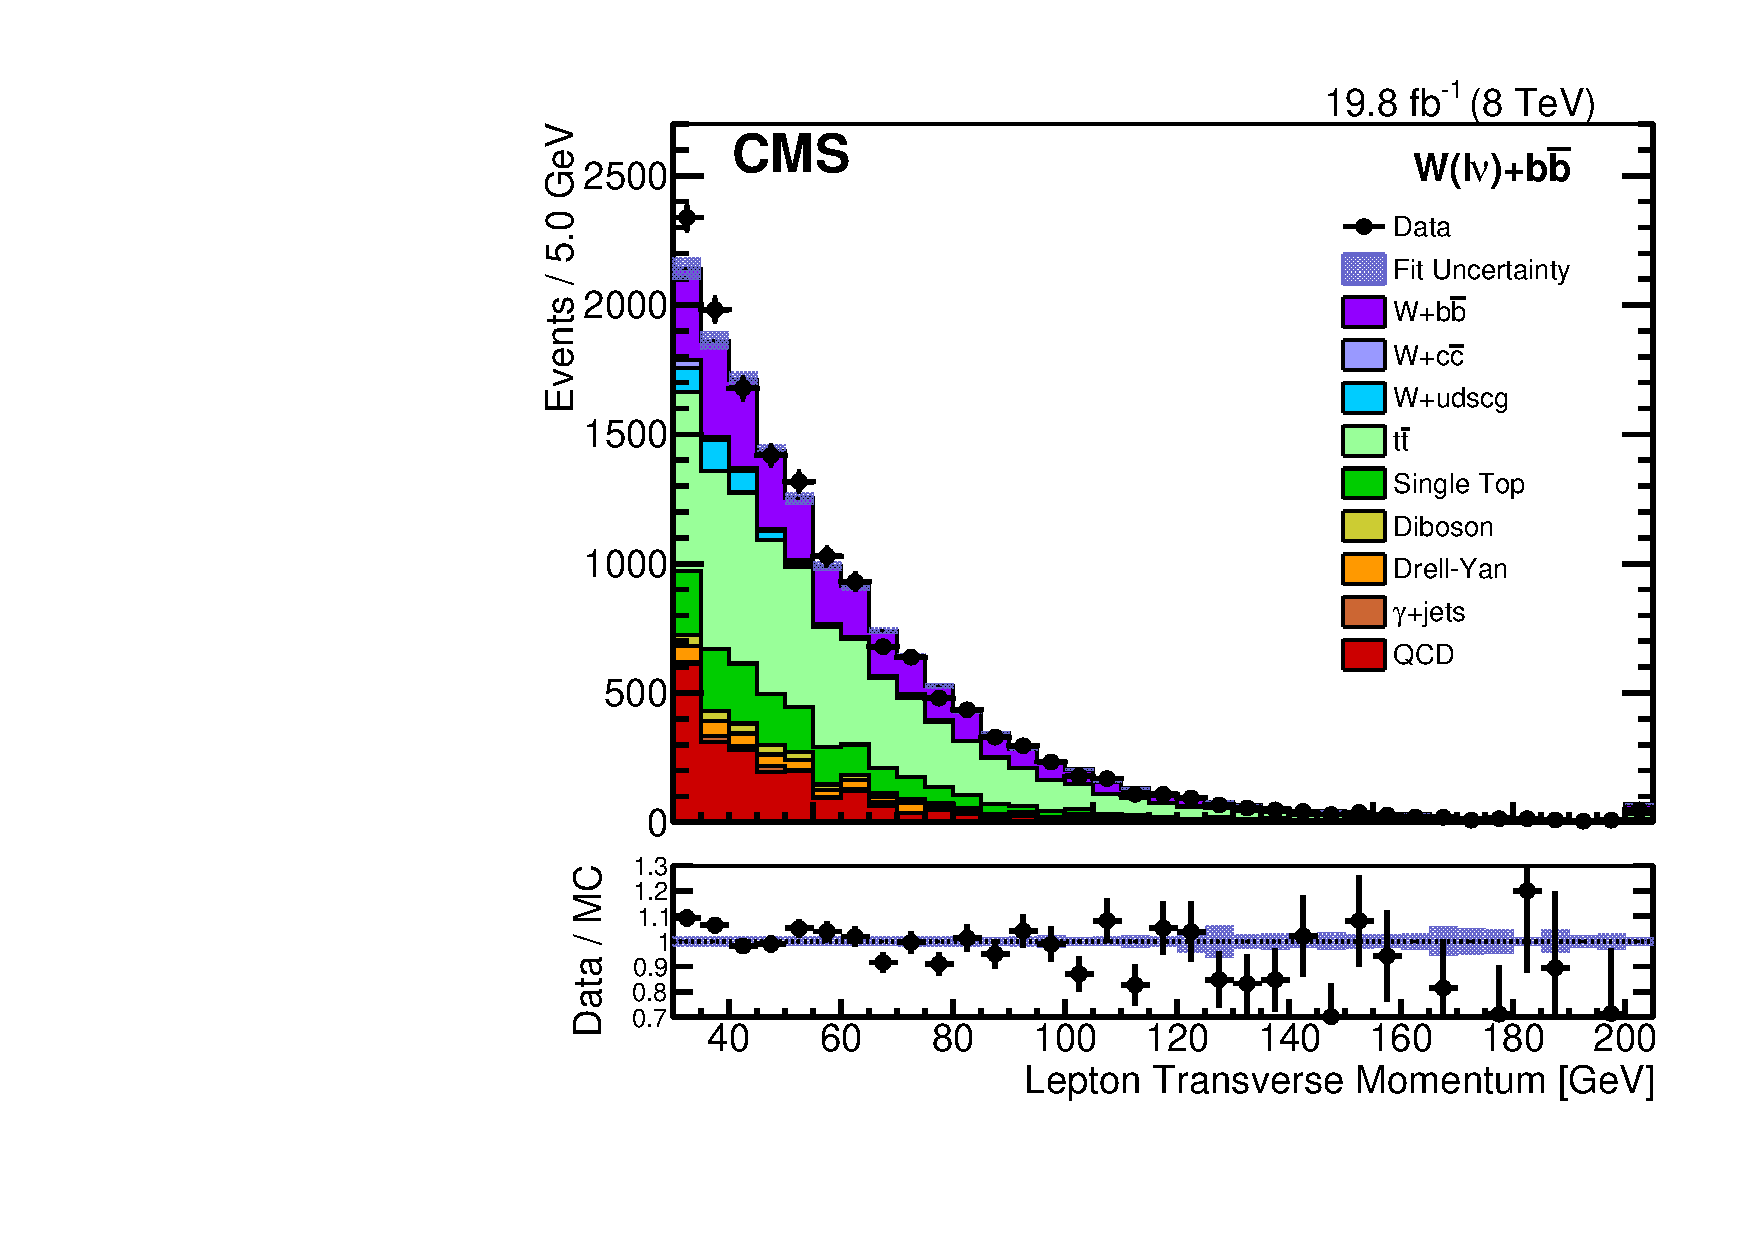
\includegraphics[width=0.49\textwidth]{/Users/rhombus/CMS/Thesis/thesis/pdfs/wbbxc/pape/postcfit_wbb_pTLep}
\label{fig:postfit_drbb_ptl}
\end{figure}

\section{Cross Section and Comparisons}

The cross section for the $\wbb$ process,
 $\sigma(\ppwbb)$,
 is derived from the signal strength measurement as obtained from the fit.
The cross section is written as

$$\sigma(\ppwbb) = 
\frac{N^{\mathrm{Data}}_{\mathrm{signal}}}{A\cdot\epsilon\cdot \mathcal{L}} = 
\frac{N^{\mathrm{Data}}_{\mathrm{signal}}}{(N^{\mathrm{MC}}_{\mathrm{signal}}/N^{\mathrm{MC}}_{\mathrm{generated}})\cdot \mathcal{L}} =
%\frac{N_{\mathrm{signal}}}{N_{\mathrm{rec}}} \cdot \frac{N_{\mathrm{gen}}}{\mathcal{L}} = 
\alpha \sigma_{\mathrm{gen}}$$
 where
 $N^{\mathrm{Data}}_{\mathrm{signal}}$ is the number of observed signal events,
 $N^{\mathrm{MC}}_{\mathrm{signal}}$ is the number of expected signal events from simulation,
 $N^{\mathrm{MC}}_{\mathrm{generated}}$ is the number of generated events in the fiducial region,
 $A$, $\epsilon$ are the acceptance and efficiency correction factors,
 $\alpha$ is the measured signal strength in the given lepton channel, and
 $\sigma_{\mathrm{gen}}$ is the simulated fiducial cross section of the signal sample.

In this analysis, the fiducial cross section was calculated in the following manner:
 Madgraph is used to compute the $\wbb$ cross section with fiducial cuts applied.
Then a k-factor for inclusive W production is applied, obtained from the ratio
of the inclusive W cross sections calculated with \FEWZ (at NNLO using the five-flavour
\CTEQ6M PDF set) and with Madgraph.
%In this analysis, the cross section used was calculated with \textsc{fewz} at NNLO
% using the five-flavor \CTEQ6M PDF set on the inclusive $\wjets$ sample.
The product $A\cdot\epsilon$ is 11~(13)\% in the
 muon (electron) channels and results from the
 combined effect of the efficiency from
 lepton identification requirements (80\%), and b tag efficiency (40\% per jet).
The uncertainty on this product is 10\% as listed in the bottom row of
 Table \ref{tab:input_unc_wbb}, which was calculated by varying the PDF
 set using the LHAPDF/PDF4LHC \cite{LHAPDF,Botje:2011sn,Alekhin:2011sk,Ball:2012cx}
 prescription considering
 PDF sets from \CTEQ, \MSTW, \NNPDF, and \HERA
 as well as varying the
 choice of scales
 $\mu_{\mathrm{F}}$, $\mu_{\mathrm{R}}$ simultaneously
 up and down by a factor of two.

The $\wbb$ cross section is measured within a fiducial volume, which is defined by
requiring leptons with $\pt > 30\GeV$ and $\abs{\eta}<2.1$ and exactly two b-tagged jets of
 $\pt > 25\GeV$ and $\abs{\eta}<2.4$.
The measured cross sections are presented in Table \ref{tab:crosssections}.
The combination of the muon and electron measurements is done using a simultaneous fit to both channels,
 taking into account correlations between different sources of uncertainties.

\begin{table}[htbp]
\begin{center}
\caption[Measured cross sections for \ppwbblnbb]{
 Measured cross sections in the muon, electron, and combined lepton channels.}
\label{tab:crosssections}
 \begin{tabular}{l|c}
 Channel        & $\sigma(\ppwbb)$, pb \\

\hline
     Muon & $  0.62 \pm 0.04 \mathrm{(stat)} \pm 0.14 \mathrm{(syst)} \pm 0.06 \mathrm{(theo)} \pm 0.02 \mathrm{(lumi)} $ \\
 Electron & $  0.69 \pm 0.05 \mathrm{(stat)} \pm 0.19 \mathrm{(syst)} \pm 0.07 \mathrm{(theo)} \pm 0.02 \mathrm{(lumi)} $ \\
 Combined & $  0.66 \pm 0.03 \mathrm{(stat)} \pm 0.14 \mathrm{(syst)} \pm 0.07 \mathrm{(theo)} \pm 0.02 \mathrm{(lumi)} $ \\
 \end{tabular}
\end{center}
\end{table}


% 
The measured cross sections are compared to theoretical predictions from
 \MCFM \cite{Campbell:2010ff, Badger:2010mg}
 with the {\MSTW2008} PDF set, as well as from
 %with the {\MSTW2008} NNLO PDF set, as well as from
 \MADGRAPH5
 interfaced with \PYTHIAs in the four- and five-flavour schemes and
 \MADGRAPH5 with \PYTHIAe \cite{ref:Pythia8} in the four-flavour scheme.
In the five-flavour scheme, the PDF set {\CTEQ6L} was
 used and \PYTHIAs was run using {TuneZ2*}.
The two four-flavour samples were produced using
 a NNLO PDF set interfaced with %NNLO23\_lo\_as\_0130\_qed
 \PYTHIA (version 6 in one sample, version 8 in the other)
 in the {CUETP8M1} tune.

% motivation
Comparisons between the results of calculations performed
 under different assumptions provide important feedback
 on the functioning and validity of the techniques employed.
Differences in predictions arising from the modelling of
 b quarks as massive or massless are possible, as are
 variations in predictions arising from the use of different
 showering packages (\PYTHIAs vs.\ \PYTHIAe) or matrix element
 generators (\MADGRAPH vs.\ \MCFM).
In the phase space explored here, these predictions are all
 very close in their central value and agree with each other
 well within their respective uncertainties.

% b -> B
The \MCFM cross section calculation is
 performed at the level of parton jets and thus
 requires a hadronization correction.
The multiplicative hadronization correction factor $0.81\pm0.07$
 is calculated using the \MADGRAPH + \PYTHIAs sample
 and agrees well with a
 similar factor calculated in the $7\TeV$ Z+b analysis
 calculated as $0.84\pm0.03$  \cite{Chatrchyan:2014dha}.
The correction factor is obtained for
 jets computed excluding neutrinos from the particle list, as
 such jets are closer in kinematics
 to particle jets at the detector level.
The uncertainty reflects both the statistics of the
 \MADGRAPH + \PYTHIAs sample as well as a comparison with the
 \MADGRAPH + \PYTHIAe sample.

% DPS
The \MCFM and four-flavour \MADGRAPH predictions do not account for
 \wbb production where the \bbbar system comes from multiple parton scattering.
CMS simulations of \MADGRAPH + \PYTHIA events that include
 double parton interaction (DPS) reproduce the $\wjets$ data \cite{Chatrchyan:2013xxa},
 therefore a \MADGRAPH + \PYTHIAe sample of a $\w$ boson produced in association with a
 \bbbar pair coming from DPS
 was generated to study the effect on the fiducial cross section.
Using this dedicated sample, an additive correction $\sigma_{\mathrm{DPS}}$
 is estimated to be $0.06\pm0.06$ pb, where the uncertainty
 is conservatively assigned to be 100$\%$ of the value.

% PDF/scale uncertainty
The uncertainty in the theoretical cross sections arising
 from the choice of PDF is also accounted for,
 using the LHAPDF/PDF4LHC \cite{LHAPDF,Botje:2011sn,Alekhin:2011sk,Ball:2012cx}
 prescription in which
 PDF sets from \CTEQ, \MSTW, \NNPDF, and \HERA are considered.
Uncertainties in the theoretical cross section due to the
 choice of scale are also estimated by varying the scales
 $\mu_{\mathrm{F}}$, $\mu_{\mathrm{R}}$ simultaneously
 up and down by a factor of two.

The resulting cross section predictions in the fiducial
 phase space at the hadron level and including the estimated
 hadronization and DPS corrections when needed
 are compared in Fig. \ref{fig:xc_comparison}
 with the measured value.
Within one standard deviation the predictions agree with the measured cross section.
The results also agree within one standard deviation with previously published $\wbb$
 measurements at 7 \TeV, where
 data are found to be well described by the same predictions.

\begin{figure}[htbp]
\caption[Cross section comparison for \wbb and generators]{
 Comparison between the measured \wbb cross section and
  various QCD predictions.
 The blue error bars on the predictions represent the uncertainty in
  the given sample associated with PDF choice and
  the black bars represent the total uncertainty.
 In the case of the \MADGRAPH + \PYTHIAs (5F) sample,
  the effects of DPS are already included in the generated
  sample so the extra DPS factor was not needed and the blue
  and black error bars overlap perfectly.
 }
\center
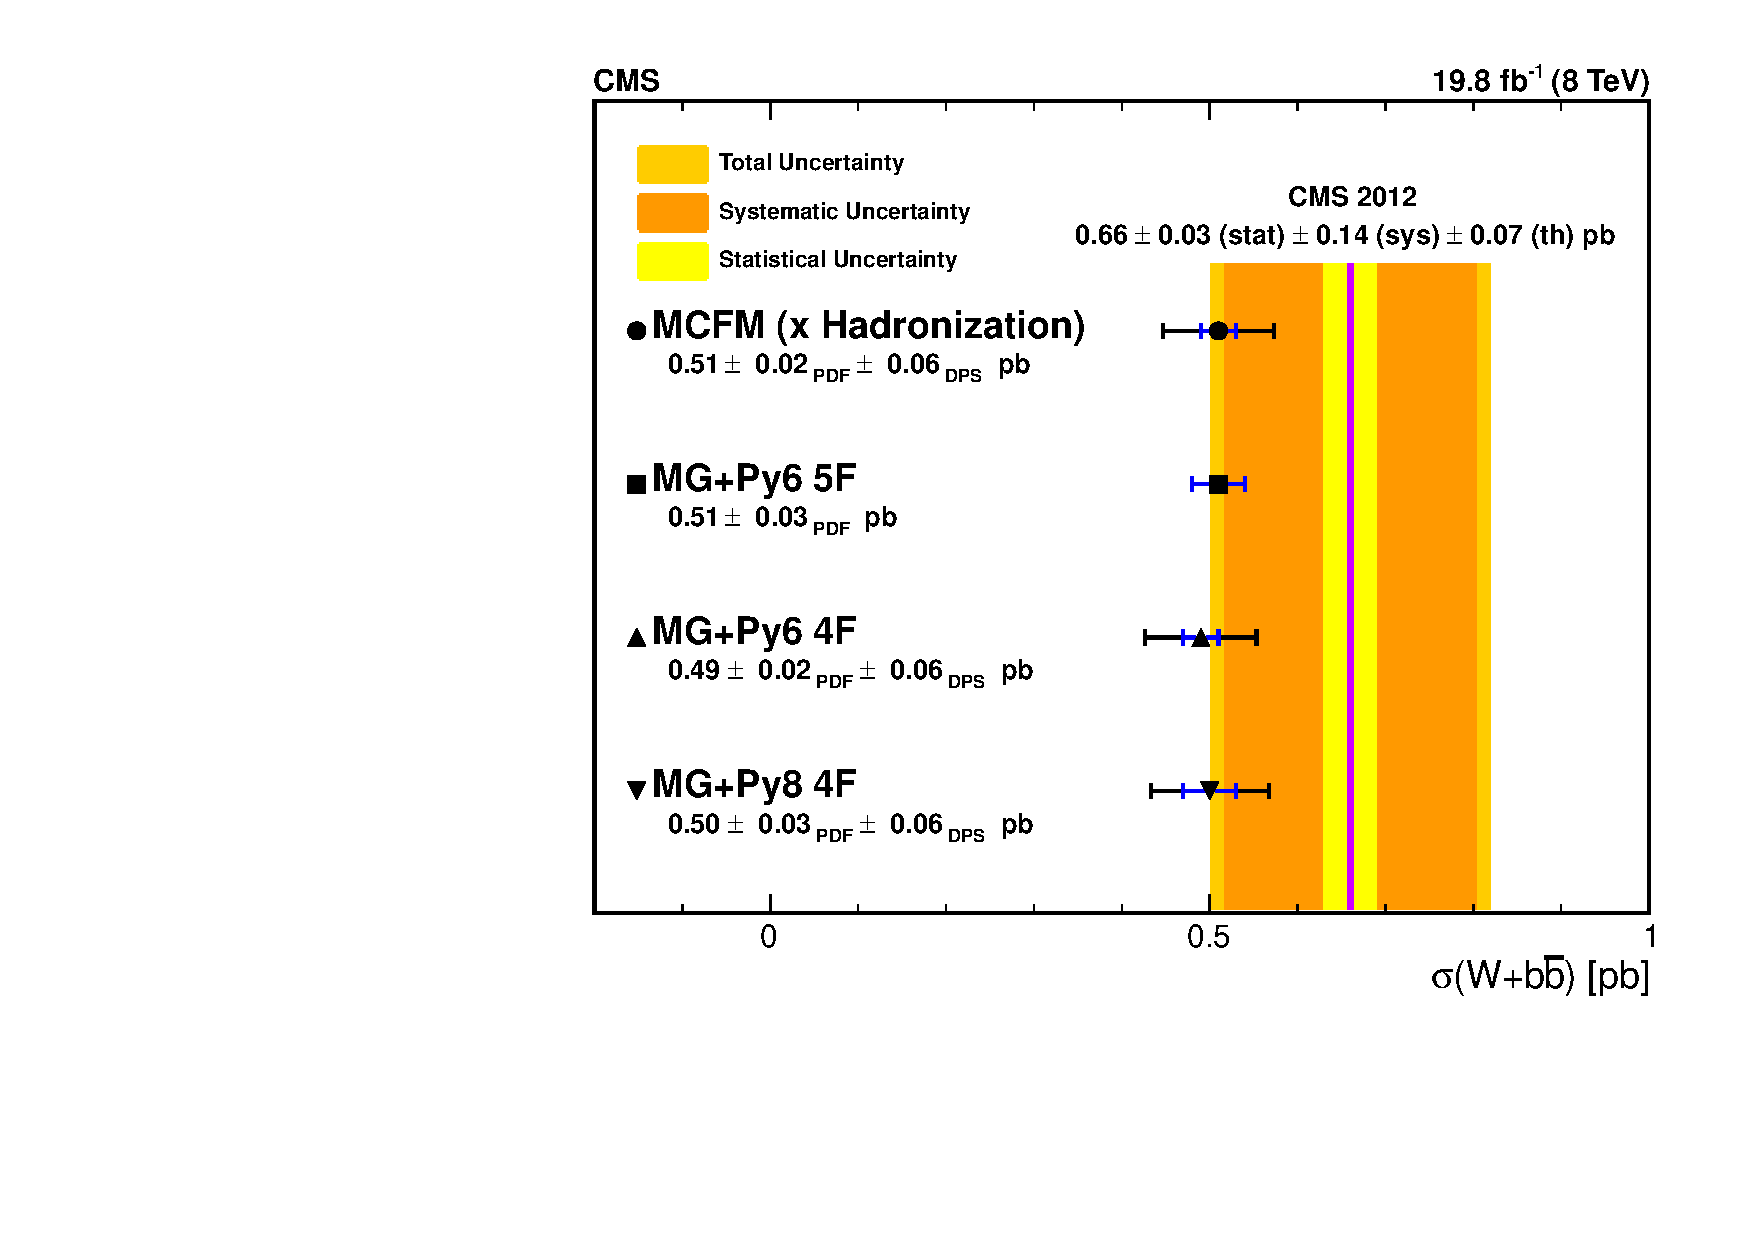
\includegraphics[width=0.7\textwidth]{/Users/rhombus/CMS/Thesis/thesis/pdfs/wbbxc/pape/MCXC_Comparison}
\label{fig:xc_comparison}
\end{figure}

